\documentclass[a4paper,twoside]{article}
\usepackage[T1]{fontenc}
\usepackage[bahasa]{babel}
\usepackage{graphicx}
\usepackage{graphics}
\usepackage{float}
\usepackage[cm]{fullpage}
\pagestyle{myheadings}
\usepackage{etoolbox}
\usepackage{setspace} 
\usepackage{lipsum} 
\setlength{\headsep}{30pt}
\usepackage[inner=2cm,outer=2.5cm,top=2.5cm,bottom=2cm]{geometry} %margin

\usepackage{url}
\usepackage{listings}%untuk penulisan source code
% \pagestyle{empty}

\makeatletter
\renewcommand{\@maketitle} {\begin{center} {\LARGE \textbf{ \textsc{\@title}} \par} \bigskip {\large \textbf{\textsc{\@author}} }\end{center} }
\renewcommand{\thispagestyle}[1]{}
\markright{\textbf{\textsc{Laporan Perkembangan Pengerjaan Skripsi\textemdash Sem. Ganjil 2015/2016}}}

\onehalfspacing
 
\begin{document}

\title{\@judultopik}
\author{\nama \textendash \@npm} 

%ISILAH DATA DATA BERIKUT INI:
\newcommand{\nama}{Priambodo Pangestu}
\newcommand{\@npm}{2013730055}
\newcommand{\tanggal}{22/11/2017} %Tanggal pembuatan dokumen
\newcommand{\@judultopik}{Pemanfaatan Smartphone Sebagai Pengendali Permainan Berbasis Web} % Judul/topik anda
\newcommand{\kodetopik}{PAN4301}
\newcommand{\jumpemb}{1} % Jumlah pembimbing, 1 atau 2
\newcommand{\pembA}{Pascal Alfadian Nugroho}
\newcommand{\pembB}{-}
\newcommand{\semesterPertama}{43 - Ganjil 17/18} % semester pertama kali topik diambil, angka 1 dimulai dari sem Ganjil 96/97
\newcommand{\lamaSkripsi}{1} % Jumlah semester untuk mengerjakan skripsi s.d. dokumen ini dibuat
\newcommand{\kulPertama}{Skripsi 1} % Kuliah dimana topik ini diambil pertama kali
\newcommand{\tipePR}{B} % tipe progress report :
% A : dokumen pendukung untuk pengambilan ke-2 di Skripsi 1
% B : dokumen untuk reviewer pada presentasi dan review Skripsi 1
% C : dokumen pendukung untuk pengambilan ke-2 di Skripsi 2
\maketitle

\pagenumbering{arabic}

\section{Data Skripsi} %TIDAK PERLU MENGUBAH BAGIAN INI !!!
Pembimbing utama/tunggal: {\bf \pembA}\\
Pembimbing pendamping: {\bf \pembB}\\
Kode Topik : {\bf \kodetopik}\\
Topik ini sudah dikerjakan selama : {\bf \lamaSkripsi} semester\\
Pengambilan pertama kali topik ini pada : Semester {\bf \semesterPertama} \\
Pengambilan pertama kali topik ini di kuliah : {\bf \kulPertama} \\
Tipe Laporan : {\bf \tipePR} -
\ifdefstring{\tipePR}{A}{
			Dokumen pendukung untuk {\BF pengambilan ke-2 di Skripsi 1} }
		{
		\ifdefstring{\tipePR}{B} {
				Dokumen untuk reviewer pada presentasi dan {\bf review Skripsi 1}}
			{	Dokumen pendukung untuk {\bf pengambilan ke-2 di Skripsi 2}}
		}

\section{Detail Perkembangan Pengerjaan Skripsi}
Detail bagian pekerjaan skripsi sesuai dengan rencan kerja/laporan perkembangan terkahir :
	\begin{enumerate}
		\item Melakukan studi literatur mengenai \textit{WebSockets}, \textit{Socket.io}, \textit{Node.js}, \textit{Canvas API}, dan \textit{Express.js}.\\
		{\bf status :} Ada sejak rencana kerja skripsi, dan ada penambahan studi literatur mengenai \textit{Express.js} pada semester ini, serta perubahan tulisan \textit{HTMLCanvas} pada rencana kerja menjadi \textit{Canvas API}.\\
		{\bf hasil :} \\
		\begin{enumerate}
			\item \textbf{Node.js} \\
			\textit{Node.js} adalah \textit{JavaScript runtime} yang dibangun berdasarkan \textit{V8} yang merupakan \textit{JavaScript engine} milik perusahaan \textit{Google} \cite{nodejs}. \textit{Node.js} memiliki model \textit{event-driven}, dan \textit{non-blocking I/O} yang membuat teknologi tersebut efisien dalam implementasinya. Teknologi ini menyediakan beberapa kelas yang berfungsi untuk mengimplementasi fitur-fitur yang dimiliki.
			
			Beberapa kelas yang terdapat pada \textit{Node.js} yaitu sebagai berikut:
			
			\textbf{HTTP} \\
			\textit{Interfaces} \textit{HTTP} pada \textit{Node.js} digunakan untuk menangani \textit{request} dari protokol \textit{HTTP} yang secara \textit{native} sulit untuk digunakan. \textit{Interface} ini akan menangani protokol \textit{HTTP} dengan tidak melakukan \textit{buffer} pada seluruh \textit{request} atau \textit{responses}.
			
			Berikut akan dijelaskan kelas-kelas yang ada pada \textit{interface} \textit{HTTP}.
			
			\begin{itemize}
				\item \textbf{http.IncomingMessage} \\ 
				Objek dari kelas ini akan dibuat oleh kelas \textit{http.Server} atau \textit{http.ClientRequest} dan memasukannya sebagai argumen suatu \textit{event} \textit{'request'} dan \textit{'response'}. Objek tersebut dapat digunakan untuk mengakses status \textit{response}, \textit{headers}, dan data. Kelas ini mengimplementasi \textit{interface Readable Stream}, beserta \textit{method, events,} dan properti yang ada didalamnya.
				
				\textbf{Properti:}
				\begin{itemize}
					\item \textbf{message.headers} \\ \textbf{Kembalian:} \textit{headers} milik objek \textit{request/response.}
					\item \textbf{message.rawHeaders} \\ \textbf{Kembalian:} bentuk \textit{raw} dari \textit{headers} milik objek \textit{request/response}.
					\item \textbf{message.statusCode} \\ \textbf{Kembalian:} tiga dijit kode status \textit{HTTP response}. Contoh: 404.
					\item \textbf{message.statusMessage} \\ \textbf{Kembalian:} pesan status \textit{HTTP response} Contoh: \textit{OK} atau \textit{Internal Server Error.}
					\item \textbf{message.url} \\ \textbf{Kembalian:} \textit{URL string} yang muncul pada permintaan \textit{HTTP}.
				\end{itemize}
				
				\item \textbf{http.ClientRequest} \\ 
				Objek dari kelas ini dibuat dalam kelas ini sendiri dan dikembalikan dari \textit{method http.request()}. Objek ini merepresentasikan permintaan yang sedang berlangsung dimana \textit{header} objek tersebut sudah berada dalam antrian. \textit{Header} masih dapat diubah dengan menggunakan \textit{setHeader(name, value)} dan \textit{removeHeader(name)}. \textit{Header} yang asli akan dikirim bersamaan dengan \textit{chunk} pertama dari suatu data atau saat memanggil \textit{request.end()}.
				
				Beberapa \textbf{event} yang dimiliki oleh kelas ini yaitu sebagai berikut:
				\begin{itemize}
					\item \textbf{'connect'} \\ Dipancarkan saat \textit{server} merespon kepada permintaan.
					\item \textbf{'response'} \\ Dipancarkan saat suatu respon diterima atas permintaan saat ini.
					\item \textbf{'timeout'} \\ Dipancarkan saat suatu \textit{socket} telah mencapai batas waktu untuk tidak aktif.
				\end{itemize}
				
				Beberapa \textit{method} yang dimiliki oleh kelas ini yaitu sebagai berikut:
				\begin{itemize}
					\item \textbf{request.end([data[,encoding]][,callback])} \\ 
					\textbf{Parameter:} 
					\begin{itemize}
						\item \textbf{data} \\tipe: \textbf{string} atau \textbf{Buffer} \\ Data yang akan dikirim.
						\item \textbf{encoding} \\tipe: \textbf{string} \\ Bersifat opsional dan akan bernilai \textit{utf8} apabila tipe parameter \textit{data} berupa \textit{string}.
						\item \textbf{callback} \\tipe:	\textbf{Function} \\ Fungsi callback
					\end{itemize}
					
					\textit{Method} ini akan mengakhiri proses pengiriman permintaan.
					
					\item \textbf{request.getHeader(name)} \\
					\textbf{Parameter:} 
					\begin{itemize}
						\item \textbf{name} \\tipe: \textbf{string} \\ Nama dari \textit{header} yang dibutuhkan.
					\end{itemize}
					\textbf{Kembalian:} suatu \textit{string} yang sesuai dengan parameter.
					
					\textit{Method} ini akan membaca seluruh \textit{header} dalam permintaan dan mengembalikan bagian yang sesuai dengan parameter. Berikut contoh implementasi dari \textit{method} ini:
\begin{lstlisting}
const contentType = request.getHeader('Content-Type');
\end{lstlisting}
					
					\item \textbf{request.removeHeader(name)} \\ 
					\textbf{Parameter:}
					\begin{itemize}
						\item \textbf{name} \\tipe: \textbf{string} \\ Nama dari \textit{header} yang dibutuhkan.
					\end{itemize}
					\textit{Method} ini akan menghapus \textit{header} yang sudah ada pada objek \textit{header}. Berikut contoh implementasi dari \textit{method} ini:
\begin{lstlisting}
request.removeHeader('Content-Type');
\end{lstlisting}
					
					\item \textbf{request.setHeader(name, value)} \\ 
					\textbf{Parameter:}
					\begin{itemize}
						\item \textbf{name} \\tipe: \textbf{string} \\ Nama dari \textit{header} yang dibutuhkan.
						\item \textbf{value} \\tipe: \textbf{value} \\ Nilai yang akan dimasukan pada objek \textit{header}
					\end{itemize}
					
					\textit{Method} ini akan menetapkan suatu nilai kepada objek \textit{header}. Berikut contoh implementasi \textit{method} ini:
\begin{lstlisting}
request.setHeader('Content-Type', 'application/json');
\end{lstlisting}
				\end{itemize}
				
				\item \textbf{http.Server} \\ 
				Kelas ini merupakan turunan dari \textit{net.Server}. \textit{Event} yang dimiliki kelas ini yaitu sebagai berikut:
				\begin{itemize}
					\item \textbf{'close'} \\ Dipancarkan apabila \textit{server} sudah ditutup.
					
				\end{itemize}
				
				Beberapa properti yang dimiliki oleh kelas ini yaitu:
				\begin{itemize}
					\item \textbf{server.listening} \\ Mengembalikan \textit{boolean} yang menandakan apakah \textit{server} melakukan proses \textit{listening} untuk suatu koneksi atau tidak.
					
					\item \textbf{server.maxHeadersCount} \\ Mengembalikan \textit{number} yang menandakan batas maksimum suatu \textit{headers} yang masuk. Nilai default dari properti ini yaitu 2000.
					
					\item \textbf{server.timeout} \\ Mengembalikan \textit{number} yang menandakan \textit{timeout} dalam milidetik.
				\end{itemize}
				
				Beberapa \textit{Method} yang dimiliki oleh kelas ini yaitu:
				\begin{itemize}
					\item \textbf{server.listen()} \\ Memulai \textit{server HTTP} melakukan proses \textit{listening} untuk suatu koneksi.
					
					\item \textbf{server.setTimeout([msecs][,callback])} \\ \textbf{Parameter:}
					\begin{itemize}
						\item \textbf{msec} nilai \textit{timeout} dalam milidetik. secara default bernilai 120000 (2 menit).
						\item \textbf{callback} fungsi \textit{callback}.
					\end{itemize}
					\textbf{Kembalian:} objek \textit{server}.
					
					\textit{Method} ini menetapkan nilai \textit{timeout} untuk \textit{sockets} dan memancarkan \textit{event 'timeout'} pada objek \textit{Server}.
					
					\item \textbf{server.close([callback])} \\ \textbf{Parameter:}
					\begin{itemize}
						\item \textbf{callback} fungsi \textit{callback}.
					\end{itemize} 
					
					\textit{Method} ini menghentikan \textit{server} untuk menerima koneksi baru.
				\end{itemize}
			\end{itemize} 
			
			Beberapa \textit{Method} yang dimiliki oleh \textit{HTTP} yaitu sebagai berikut:
			\begin{itemize}
				\item \textbf{http.createServer([requestListener])} \\ \textbf{Parameter:}
				\begin{itemize}
					\item \textbf{requestListener} fungsi yang akan secara otomatis ditambahkan pada \textit{event} \textit{'request'} milik kelas \textit{http.Server}.
				\end{itemize}
				\textbf{Kembalian:} objek \textit{http.Server}
				
				\textit{Method} ini akan membuat objek \textit{http.Server} untuk menangani \textit{request} dari \textit{client} dan memberikan \textit{response} kepada \textit{client}. Fungsi yang diberikan pada \textit{method} ini akan dipanggil satu kali setiap \textit{request} dibuat kepada \textit{server}.
				
				\item \textbf{http.request(options[,callback])} \\ 
				\textbf{Parameter:}
				\begin{itemize}
					\item \textbf{options} \\ Dapat berupa \textit{Object, string} atau \textit{URL}. Berikut jenis-jenis \textit{options} yang dapat menjadi parameter:
					\begin{itemize}
						\item \textbf{protocol} \\tipe: \textbf{string} \\ Protokol yang digunakan.
						\item \textbf{host} \\tipe: \textbf{string} \\ Nama domain atau alamat \textit{IP} milik server.
						\item \textbf{hostname} \\tipe: \textbf{string} \\ Nama lain untuk \textit{host}.
						\item \textbf{port} \\tipe: \textbf{number} \\ \textit{Port} untuk \textit{server}.
						\item \textbf{path} \\tipe: \textbf{string} \\ \textit{Path} untuk permintaan.
						\item \textbf{headers} \\tipe: \textbf{Object} \\ Objek yang berisi permintaan \textit{headers}.
						\item \textbf{timeout} \\tipe: \textbf{number} \\ Nomor yang menentukan \textit{timeout} dari suatu \textit{socket} dalam milidetik.
					\end{itemize}
					
					\item \textbf{callback} \\tipe: \textbf{Function} \\ Fungsi \textit{callback}.
				\end{itemize}
				
				\textbf{Kembalian:} objek dari kelas \textit{http.ClientRequest}.
				
				\textit{Method} ini digunakan untuk menangani permintaan \textit{HTTP} pada \textit{server}. Berikut contoh implementasi dari \textit{method} ini:
\begin{lstlisting}
const options = {
hostname: 'www.google.com',
port: 80,
path: '/upload',
method: 'POST',
headers: {
	'Content-Type': 'application/x-www-form-urlencoded',
	'Content-Length': Buffer.byteLength(postData)
	}
};
				
const req = http.request(options, (res) => {
console.log(`STATUS: ${res.statusCode}`);
console.log(`HEADERS: ${JSON.stringify(res.headers)}`);
res.setEncoding('utf8');
res.on('data', (chunk) => {
console.log(`BODY: ${chunk}`);
});
res.on('end', () => {
console.log('No more data in response.');
});
});
				
req.end();
\end{lstlisting}	
			\end{itemize}
			
			%THIS IS EVENTS CLASS
			\textbf{Events} \\
			\textit{Node.js} dibangun berdasarkan arsitektur \textit{event-driven} dengan sifat \textit{asynchronous}, dimana jenis-jenis objek tertentu akan memancarkan suatu \textit{events} secara berkala dan akan memanggil objek \textit{Function} ("\textit{listeners}").
			
			Semua objek yang memancarkan \textit{events} merupakan turunan dari kelas \textit{EventEmitter}. Objek tersebut akan memanggil \textit{method} \textit{eventEmitter.on()} yang memungkinkan satu atau beberapa fungsi dapat ditangani dalam suatu \textit{event} yang dipancarkan oleh objek saat ini.
			
			Kelas \textit{EventEmitter} dapat didefinisikan dengan memanggil modul \textit{events} seperti berikut :
			
\begin{lstlisting}
const EventEmitter = require('events');
\end{lstlisting}
			
			Sebuah \textit{EventEmitter} akan memancarkan \textit{'event'} \textit{'newListener'} pada saat \textit{listeners} baru akan ditambahkan, dan \textit{'removeListener'} akan dipancarkan saat \textit{listeners} saat ini akan dihapus.
			
			Berikut merupakan beberapa \textit{method} yang dimiliki oleh kelas \textit{EventEmitter}:
			
			\begin{itemize}
				\item \textbf{eventEmitter.on(eventName, listener)} \\ \textbf{Parameter:}
				\begin{itemize}
					\item \textit{eventName}, nama dari suatu \textit{event} yang akan dipancarkan.
					\item \textit{listener}, suatu fungsi \textit{callback} yang akan menangani \textit{event} dari \textit{eventName}. 
				\end{itemize} 
				\textbf{Kembalian:} referensi kepada \textit{EventEmitter}.
				
				\textit{Method} ini berfungsi untuk mencatat suatu listener yang akan digunakan. Fungsi \textit{listener} yang menjadi parameter \textit{method} ini akan ditambahkan ke \textit{index} terakhir dari \textit{array of listeners} pada \textit{eventName}. Tidak akan ada pengecekan apakah fungsi \textit{listener} sudah dimasukan sebelumnya. Oleh karena itu, pemanggilan \textit{eventName} dan \textit{listener} secara berulang akan menyebabkan fungsi \textit{listener} dimasukan kedalam \textit{array} dan dipanggil secara berulang. \textit{Method} ini juga akan mengembalikan \textit{reference} kepada \textit{EventEmitter}, sehingga pemanggilan dapat saling menyambung dengan pemanggilan lainnya.
				
				Berikut merupakan contoh implementasi dari \textit{method} ini:
\begin{lstlisting}
const EventEmitter = require('events');
				
class MyEmmit extends EventEmitter {}
				
const myEmmit = new MyEmitter();
				
myEmmit.on('event', () => {
console.log('suatu event telah terjadi');	
});
\end{lstlisting}
				
				\item \textbf{eventEmitter.emit(eventName)} \\ \textit{Method} ini berfungsi untuk memicu suatu \textit{event} yang akan dipancarkan. \textbf{Parameter:}
				\begin{itemize}
					\item \textit{eventName}, nama dari sebuah \textit{event} yang akan dipancarkan.
					\item \textit{...args}, argumen tambahan yang akan diberikan pada \textit{eventName}. 
				\end{itemize}
				\textbf{Kembalian:} \textit{true} apabila \textit{event} memiliki \textit{listener}, false jika tidak.
				
				\textit{Method} ini akan memanggil masing-masing \textit{listener} yang sudah dicatat oleh \textit{eventEmitter.on()} dalam \textit{array of listeners} secara sinkronis, dimana beberapa \textit{listener} tersebut mengacu pada \textit{eventName} yang sama. Argumen yang diterima dari parameter akan diberikan pada masing-masing \textit{listener}.
				
				Berikut merupakan contoh implementasi dari \textit{method} ini:
\begin{lstlisting}
const EventEmitter = require('events');
				
class MyEmmit extends EventEmitter {}
				
const myEmmit = new MyEmitter();
				
myEmmit.on('event', () => {
console.log('suatu event telah terjadi');	
});
myEmitter.emit('event');
\end{lstlisting} 
			\end{itemize}
			
			%THIS IS STREAMS CLASS
			\textbf{Streams} \\
			Kelas ini digunakan untuk menangani aliran data yang terjadi pada \textit{Node.js}. Data yang ditangani dapat berjumlah banyak dan akan menghabiskan banyak memori apabila tidak ditangani dengan baik. Oleh karena itu, modul \textit{stream} menyediakan fitur-fitur yang memudahkan penanganan aliran data.
			
			Ada empat tipe dasar \textit{stream} dalam \textit{Node.js}:
			\begin{itemize}
				\item \textbf{Readable} \\ \textit{Streams} yang dapat membaca data dari sumber eksternal tertentu.
				\item \textbf{Writable} \\ \textit{Streams} yang dapat menulis data dan mengirimkannya ke sumber external tertentu.
				\item \textbf{Duplex} \\ \textit{Streams} yang dapat membaca dan menulis data sekaligus.
				\item \textbf{Transform} \\ \textit{Duplex streams} yang dapat memodifikasi atau mengubah data dimana data tersebut dapat dilihat langsung hasil perubahannya.
			\end{itemize}
			
			\begin{enumerate}
				\item \textbf{Readable Stream} \\
				Merupakan abstraksi untuk sumber data yang digunakan. Berikut merupakan contoh dari \textit{Readable Stream} pada \textit{Node.js}:
				\begin{itemize}
					\item \textbf{HTTP responses} pada \textit{client}
					\item \textbf{HTTP requests} pada \textit{server}
					\item \textbf{fs read streams}
				\end{itemize}
				Seluruh \textit{Readable streams} mengimplementasi \textit{interface} yang didefinisikan oleh kelas \textit{stream.Readable}.
				
				\begin{itemize}
					\item \textbf{stream.Readable} \\
					\textbf{Events:}
					\begin{itemize}
						\item \textbf{'close'} \\ \textit{Event} ini dipancarkan saat suatu \textit{stream} atau sumber lain telah ditutup. \textit{Event} ini menandakan tidak akan ada \textit{event} lagi yang akan dipancarkan, dan tidak ada komputasi lain yang akan dilakukan.
\begin{lstlisting}
const readable = getReadableStreamSomehow();
readable.on('close', (chunk) => {
console.log(`Stream telah ditutup`);
});
\end{lstlisting}
						
						\item \textbf{'data'} \\ \textit{Event} ini akan dipancarkan setiap kali suatu \textit{stream} melepas kepemilikan sebuah data kepada pemakai. Hal tersebut dapat terjadi setiap suatu \textit{stream} berganti menjadi mode \textit{flowing} dengan memanggil \textit{readable.pipe()}, \textit{readable.resume()}, atau dengan menghubungkan \textit{listener callback} pada \textit{'data' event}. Contoh implementasi:
\begin{lstlisting}
const readable = getReadableStreamSomehow();
readable.on('data', (chunk) => {
console.log(`Menerima data sebesar ${chunk.length} bytes.`);
});
\end{lstlisting}
						
						\item \textbf{'end'} \\ \textit{Event} ini dipancarkan saat tidak ada lagi data yang akan digunakan dari \textit{stream}. Contoh implementasi:
\begin{lstlisting}
const readable = getReadableStreamSomehow();
readable.on('end', () => {
console.log('Tidak akan ada data yang dikirimkan.');
});
\end{lstlisting}
						
						\item \textbf{'error'} \\ \textit{Event} ini akan dipancarkan oleh \textit{Readable} setiap saat. \textit{Event} ini dapat terjadi apabila \textit{stream} tidak dapat menyediakan data dikarenakan kesalahan internal, atau ketika implementasi suatu \textit{stream} mencoba mengirimkan \textit{chunk} dari data yang tidak sesuai. Contoh implementasi:
\begin{lstlisting}
const readable = getReadableStreamSomehow();
readable.on('error', () => {
console.error('Terjadi kesalahan');
});
\end{lstlisting}
						
						
					\end{itemize}
					
					\textbf{Method:}
					\begin{itemize}
						\item \textbf{readable.pipe(destination[, options])} \\ \textbf{Parameter:}
						\begin{itemize}
							\item \textbf{destination} \\tipe: \textit{stream.Writable} \\ Destinasi untuk menulis suatu data.
							\item \textbf{options} \\tipe: \textit{Object} \\ Bersifat opsional, dapat berupa objek sebagai berikut:
							
								\textbf{end} \\tipe: \textit{boolean} \\ Mengakhiri \textit{writer} yang melakukan proses menulis saat \textit{reader} telah selesai. Nilai \textit{default} parameter ini yaitu \textit{true}.
							
						\end{itemize}
						\textbf{Kembalian:} referensi yang menuju \textit{destination}.
						
						\textit{Method} ini akan menghubungkan \textit{Writable stream} pada objek \textit{readable}, sehingga dapat berubah menjadi mode \textit{flowing} secara otomatis dan akan menaruh seluruh data pada \textit{Writable} yang sudah terhubung. \textit{Method} ini mengembalikan referensi yang menuju \textit{destination}, sehingga \textit{pipe streams} dapat saling menyambung dengan \textit{pipe streams} lainnya.
						
						Berikut merupakan contoh implementasi dari \textit{method} ini:
\begin{lstlisting}
const fs = require('fs');
						
const readable = getReadableStreamSomehow();
const writable = fs.createWriteStream('file.txt');
						
//seluruh data dari objek readable masuk ke 'file.txt'
readable.pipe(writable); 
\end{lstlisting}
						
					\end{itemize}
				\end{itemize}
			\end{enumerate}
			
			
			%------------- END OF NODE.JS --------------
			
			\item \textbf{Express.js} \\
			\textit{Express.js} merupakan \textit{framework} aplikasi web untuk \textit{Node.js} \cite{expressjs}. \textit{Express.js} menyediakan fitur-fitur untuk web dan aplikasi \textit{mobile} agar dapat bertahan lama. Untuk dapat menggunakan \textit{Express.js}, dapat dilakukan langkah sebagai berikut: 
\begin{lstlisting}
var express = require('express');
var app = express();
\end{lstlisting}
			
			Dengan begitu, fitur-fitur yang terdapat pada \textit{Express.js} dapat digunakan untuk pengembangan aplikasi tertentu.
			
			Berikut akan dijelaskan kelas-kelas yang terdapat pada \textit{Express.js}:
			
			\textbf{express()} \\
			Untuk membuat aplikasi \textit{Express}, langkah yang dilakukan adalah sebagai berikut:
\begin{lstlisting}
const express = require('express');
const app = express();
\end{lstlisting}
			
			\textit{Method} yang dimiliki oleh fungsi \textit{express()} yaitu sebagai berikut:
			
			\begin{itemize}
				\item \textbf{express.Router([options])} \\ \textbf{Parameter:} 
				\begin{itemize}
					\item \textbf{options} bersifat opsional dan akan menentukan sifat dari objek \textit{router}. Parameter ini dapat berupa beberapa jenis seperti berikut:
					\begin{itemize}
						\item \textit{caseSensitive} memungkinkan \textit{case-sensitive}. Dapat bernilai \textit{true} atau \textit{false}. Secara default akan bernilai \textit{false}.
						
						\item \textit{strict} memungkinkan \textit{strict routing}. Dapat bernilai \textit{true} atau \textit{false}. Apabila bernilai \textit{false}, maka parameter \textit{'/foo'} dan \textit{'/foo/'} akan dianggap sama oleh \textit{router}.
					\end{itemize}
				\end{itemize}
				
			\end{itemize}
			
			
			%THIS IS APPLICATION CLASS
			\textbf{Application} \\
			Kelas ini akan menangani berbagai proses yang terjadi dalam aplikasi \textit{Express} seperti melakukan \textit{routing} terhadap \textit{HTTP requests}, mengatur \textit{middleware}, \textit{rendering} sebuah \textit{HTML views}, dan mendaftarkan \textit{template engine} tertentu. Untuk dapat melakukan fungsi-fungsi tersebut dapat dilakukan langkah berikut:
			
\begin{lstlisting}
const express = require('express');
const app = express();
\end{lstlisting}
			
			Baris pertama dari potongan kode tersebut berarti variabel \textit{express} memanggil modul \textit{'express'} agar dapat mengakses fungsi-fungsi yang ada pada modul tersebut. Sedangkan baris kedua, Objek \textit{app} memanggil fungsi \textit{express()} yang telah didapatkan dari variabel \textit{express}.
			
			Kelas ini memiliki beberapa \textit{method} sebagai berikut:
			
			\begin{itemize}
				\item \textbf{app.all(path, callback[, callback ...])} \\ \textbf{Parameter:} 
				\begin{itemize}
					\item \textbf{path} suatu \textit{path} yang akan ditangani oleh \textit{middleware}. Dapat berupa \textit{string}, \textit{path pattern}, atau \textit{array} dari kombinasi \textit{string} dan \textit{path pattern}.
					
					\item \textbf{callback} merupakan fungsi \textit{callback}, dimana fungsi tersebut dapat berupa fungsi \textit{middleware}, kumpulan dari fungsi \textit{middleware} (yang dipisahkan dengan menggunakan koma), fungsi \textit{array of middleware}, atau kombinasi dari seluruh \textit{item} tersebut.
				\end{itemize}
				
				\textit{Method} ini dapat menangani seluruh \textit{HTTP requests} seperti \textit{GET, POST, PUT,} dan \textit{DELETE}. Berikut merupakan contoh implementasi dari \textit{method} ini:
\begin{lstlisting}
app.all('/about', function(req, res, next){
console.log('Mengakses bagian about ...');
next(); //bagian ini akan menuju ke handler berikutnya
});
\end{lstlisting}
				
				\item \textbf{app.get(path, callback[, callback ...])} \\ \textbf{Parameter:}
				\begin{itemize}
					\item \textbf{path} suatu \textit{path} yang akan ditangani oleh \textit{middleware}. Dapat berupa \textit{string}, \textit{path pattern}, atau \textit{array} dari kombinasi \textit{string} dan \textit{path pattern}.
					
					\item \textbf{callback} merupakan fungsi \textit{callback}, dimana fungsi tersebut dapat berupa fungsi \textit{middleware}, kumpulan dari fungsi \textit{middleware} (yang dipisahkan dengan menggunakan koma), fungsi \textit{array of middleware}, atau kombinasi dari seluruh \textit{item} tersebut.
				\end{itemize}
				
				\textit{Method} ini akan mengarahkan \textit{HTTP GET requests} pada \textit{path} dengan fungsi \textit{callback} tertentu. Berikut merupakan contoh implementasi dari \textit{method} ini:
\begin{lstlisting}
app.get('/', function(req, res){
res.send('Mengirimkan GET request pada homepage');
});
\end{lstlisting}
				
				\item \textbf{app.post(path, callback[, callback ...])} \\ \textbf{Parameter:}
				\begin{itemize}
					\item \textbf{path} suatu \textit{path} yang akan ditangani oleh \textit{middleware}. Dapat berupa \textit{string}, \textit{path pattern}, atau \textit{array} dari kombinasi \textit{string} dan \textit{path pattern}.
					
					\item \textbf{callback} merupakan fungsi \textit{callback}, dimana fungsi tersebut dapat berupa fungsi \textit{middleware}, kumpulan dari fungsi \textit{middleware} (yang dipisahkan dengan menggunakan koma), fungsi \textit{array of middleware}, atau kombinasi dari seluruh \textit{item} tersebut.
				\end{itemize}
				
				\textit{Method} ini akan mengarahkan \textit{HTTP POST requests} pada \textit{path} dengan fungsi \textit{callback} tertentu. Berikut merupakan contoh implementasi dari \textit{method} ini:
\begin{lstlisting}
app.post('/', function(req, res){
res.send('Mengirimkan POST requests pada homepage');
});
\end{lstlisting}
				
				\item \textbf{app.route(path)} \\ \textbf{Parameter:}
				\begin{itemize}
					\item \textbf{path} suatu \textit{path} yang akan ditangani oleh \textit{middleware}. Dapat berupa \textit{string}, \textit{path pattern}, atau \textit{array} dari kombinasi \textit{string} dan \textit{path pattern}.
				\end{itemize}
				
				\textit{Method} ini akan mengembalikan instansi dari satu \textit{route}, yang kemudian dapat digunakan untuk menangani \textit{HTTP request} dengan \textit{middleware} tertentu. Berikut merupakan contoh implementasi dari \textit{method} ini:
\begin{lstlisting}
app.route('/buku').get(function(req, res){
res.send('Mendapatkan suatu buku');
});
\end{lstlisting}
				
				\item \textbf{app.use([path,] callback[, callback...])} \\ \textbf{Parameter:} 
				\begin{itemize}
					\item \textbf{path} suatu \textit{path} yang akan ditangani oleh \textit{middleware}. Dapat berupa \textit{string}, \textit{path pattern}, atau \textit{array} dari kombinasi \textit{string} dan \textit{path pattern}.
					
					\item \textbf{callback} merupakan fungsi \textit{callback}, dimana fungsi tersebut dapat berupa fungsi \textit{middleware}, kumpulan dari fungsi \textit{middleware} (yang dipisahkan dengan menggunakan koma), fungsi \textit{array of middleware}, atau kombinasi dari seluruh \textit{item} tersebut.
				\end{itemize}
				
				\textit{Method} ini akan menghubungkan \textit{middleware} atau suatu fungsi tertentu dengan \textit{path} yang sudah ditentukan. Dalam implementasi \textit{method} ini, urutan penempatan pada baris kode sangat berpengaruh. Setelah \textit{app.use()} dieksekusi, maka suatu \textit{request} tidak akan mengeksekusi \textit{middleware} yang ada dibawah baris kode \textit{app.use()}.  Berikut merupakan contoh implementasi dari \textit{method} ini:
\begin{lstlisting}
//request hanya akan sampai pada middleware ini
app.use(function(req, res){
res.send('Hanya sampai sini saja');
});
				
//request tidak akan mengeksekusi baris ini
app.get('/', function(req, res){
res.send('Hello World!');
});
\end{lstlisting}
				
				\item \textbf{app.listen(port, [hostname], [backlog], [callback])} \\ \textbf{Parameter:}
				\begin{itemize}
					\item \textbf{port} nomor yang akan dituju oleh server.
					\item \textbf{hostname} \textit{string} yang diberikan pada gawai tertentu agar dapat dikenali. Parameter ini bersifat opsional.
					\item \textbf{backlog} nomor yang menentukan ukuran maksimal dalam antrian koneksi yang tertunda.Parameter ini bersifat opsional.
					\item \textbf{callback} merupakan fungsi \textit{callback}, dimana fungsi tersebut dapat berupa fungsi \textit{middleware}, kumpulan dari fungsi \textit{middleware} (yang dipisahkan dengan menggunakan koma), fungsi \textit{array of middleware}, atau kombinasi dari seluruh \textit{item} tersebut. Parameter ini bersifat opsional.
				\end{itemize}
				
				\textit{Method} ini akan menghubungkan suatu koneksi pada \textit{host} dan \textit{port} yang sudah ditentukan. Berikut merupakan contoh implementasi dari \textit{method} ini:
\begin{lstlisting}
const express = require('express');
const app = express();
app.listen(3000);
\end{lstlisting}
				
			\end{itemize}
			
			
			%THIS IS REQUEST CLASS
			\textbf{Request} \\
			Sebuah objek dari kelas \textit{Request} akan merepresentasikan \textit{HTTP request} dan memiliki properti untuk \textit{request query} seperti \textit{body, HTTP headers} dan \textit{parameters}.
			
			Beberapa \textit{method} yang ada pada kelas \textit{Request} yaitu: 
			\begin{itemize}
				\item \textbf{req.accepts(types)} \\ Berfungsi untuk memeriksa apakah tipe konten tertentu dapat diterima atau tidak.
				
				\item \textbf{req.get(field)} \\ Berfungsi untuk mengembalikan \textit{HTTP request header} tertentu.
				
				\item \textbf{req.is(type)} \\ Berfungsi untuk mengembalikan apakah benar atau salah \textit{type} pada parameter sama dengan status \textit{Content-Type} pada \textit{HTTP header}.
			\end{itemize}
			
			
			%THIS IS RESPONSE CLASS
			\textbf{Response} \\
			Sebuah objek dari kelas \textit{Response} akan merepresentasikan respon \textit{HTTP} yang dikirim oleh \textit{Express} pada saat menerima \textit{HTTP request}.
			
			Beberapa \textit{method} yang terdapat pada kelas \textit{Response} yaitu: 
			
			\begin{itemize}
				\item \textbf{res.send([body])} \\ \textbf{Parameter:} \textit{body} dapat berupa berbagai jenis objek seperti \textit{Buffer}, \textit{String}, dan \textit{Array}.
				
				\textit{Method} ini akan mengirimkan respon HTTP kepada \textit{client} sesuai dengan parameter yang diterima. Berikut merupakan contoh implementasi dari \textit{method} ini:
\begin{lstlisting}
//parameter objek String
res.send('Hello World!');
				
//parameter objek Array
res.send([1,2,3]);
				
//parameter objek Buffer
res.send(new Buffer('<p>This is a Buffer</p>'));
\end{lstlisting}
				
				\item \textbf{res.end([data][, encoding])} \\ \textbf{Parameter:}
				\begin{itemize}
					\item \textbf{data} dapat berupa objek \textit{String} atau \textit{Buffer} yang akan dikirim saat mengakhiri proses respon.
					\item \textbf{encoding} merubah suatu tipe data menjadi tipe data yang lain. Contoh beberapa tipe data yang tersedia yaitu \textit{utf8, base64, ascii, } dan \textit{hex}.
				\end{itemize}
				
				\textit{Method} ini berfungsi untuk mengakhiri suatu proses respon. Apabila akan mengakhiri suatu respon tanpa memerlukan suatu data, maka dapat menggunakan \textit{method} ini. Berikut merupakan contoh implementasi \textit{method} ini:
\begin{lstlisting}
app.get('/', function(req, res){
res.end(); //apabila tidak memerlukan data.

// apabila memerlukan suatu 
// data untuk mengakhiri proses.
res.end('goodbye!'); 
});
\end{lstlisting}
				
				\item \textbf{res.render(view[, locals][, callback])} \\ \textbf{Parameter:}
				\begin{itemize}
					\item \textbf{view} suatu \textit{string} yang menunjukan \textit{path} dari suatu \textit{view file}.
					\item \textbf{locals} suatu objek yang memiliki properti yang menunjukan variabel lokal dari \textit{view}.
					\item \textbf{callback} suatu fungsi \textit{callback}. 
				\end{itemize}
				
				\textit{Method} ini berfungsi untuk merubah \textit{view file} dan mengirim \textit{file} tersebut kepada \textit{client}. Berikut merupakan contoh implementasi \textit{method} ini:
\begin{lstlisting}
app.get('/', function(req, res){

//akan merubah(render) halaman about 
res.render('about');  
});
\end{lstlisting}
				
				\item \textbf{res.sendStatus(statusCode)} \\ \textbf{Parameter:} 
				\begin{itemize}
					\item \textbf{statusCode} kode status \textit{HTTP}.
				\end{itemize}
				
				\textit{Method} ini akan menetapkan kode status \textit{HTTP} di parameter, dan akan mengirimkan bentuk \textit{String} sebagai \textit{body} dari respon. Berikut contoh implementasi \textit{method} ini:
\begin{lstlisting}
// akan mengirimkan 'OK' 
// pada response body.
res.sendStatus(200); 
				
// akan mengirimkan 'Not Found' 
// pada response body.
res.sendStatus(404); 
				
// akan mengirimkan 'Internal 
// Server Error' pada response body.
res.sendStatus(500); 
\end{lstlisting}
				
				\item \textbf{res.status(code)} \\ \textbf{Parameter:}
				\begin{itemize}
					\item \textbf{code} kode status \textit{HTTP}.
				\end{itemize}
				
				\textit{Method} ini akan menetapkan kode status \textit{HTTP} untuk respon. Berikut merupakan contoh implementasi \textit{method} ini:
\begin{lstlisting}
res.status(403).end();
res.status(400).send('Bad Request');
\end{lstlisting}
				
				\item \textbf{res.json([body])} \\ \textbf{Parameter:}
				\begin{itemize}
					\item \textbf{body} dapat berupa tipe \textit{JSON} apapun, seperti \textit{array, String,} dan \textit{Boolean}.
				\end{itemize}
				
				\textit{Method} ini berfungsi untuk mengirimkan respon \textit{JSON}. Berikut merupakan contoh implementasi \textit{method} ini:
\begin{lstlisting}
res.json({ user: 'tobi', age: '27'});
\end{lstlisting}
				
			\end{itemize}
			
			
			%THIS IS ROUTER CLASS
			\textbf{Router} \\
			Objek dari kelas \textit{Router} merupakan \textit{instance} dari \textit{middleware} dan \textit{routes}. Setiap aplikasi \textit{Express} memiliki \textit{router} secara \textit{built-in}. 
			
			\textit{Method} yang dimiliki oleh \textit{Router} yaitu sebagai berikut:
			
			\begin{itemize}
				\item \textbf{router.METHOD(path, [callback, ...] callback)} \\ \textbf{Parameter:} \\ 
				\begin{itemize}
					\item \textbf{path} suatu \textit{path} yang akan ditangani oleh \textit{middleware}. Dapat berupa \textit{string}, \textit{path pattern}, atau \textit{array} dari kombinasi \textit{string} dan \textit{path pattern}.
					
					\item \textbf{callback} merupakan fungsi \textit{callback}, dimana fungsi tersebut dapat berupa fungsi \textit{middleware}, kumpulan dari fungsi \textit{middleware} (yang dipisahkan dengan menggunakan koma), fungsi \textit{array of middleware}, atau kombinasi dari seluruh \textit{item} tersebut.
				\end{itemize}
				
				\textit{Method} ini menyediakan fungsionalitas \textit{routing} dalam aplikasi \textit{Express}, dimana \textit{METHOD} merupakan salah satu \textit{HTTP methods} seperti \textit{GET, PUT, } dan \textit{POST}, dalam huruf kecil. Dengan begitu, \textit{method} ini dapat berupa \textit{router.get(), router.post(),} dan \textit{router.put()}.
				
				Berikut merupakan contoh implementasi dari \textit{method} ini:
\begin{lstlisting}
//menggunakan HTTP method GET
router.get('/', function(req, res){
res.send('hello world');
});
				
//menggunakan HTTP method POST
router.post('/buku', function(req, res){
res.send('mendapatkan buku');
});
\end{lstlisting}
				
			\end{itemize}
			
			%------------- END OF EXPRESS.JS--------------- 
			
			\item \textbf{WebSockets} \\
			\textit{WebSockets} merupakan \textit{Application Programming Interface (API)} yang memiliki kemampuan untuk membuka sesi komunikasi interaktif antara \textit{browser} pengguna dan \textit{server} \cite{websockets}. Dengan \textit{API} ini, pengguna dapat mengirim pesan ke \textit{server} dan menerima respon tanpa harus melakukan \textit{polling} pada \textit{server} terlebih dahulu.
			
			Berikut akan dijelaskan kelas-kelas yang ada pada \textit{WebSockets}:
			
			%THIS IS WEBSOCKET CLASS
			\textbf{WebSocket} \\
			Kelas ini merupakan inti untuk mengakses fungsi yang ada pada \textit{WebSockets}. Sebuah objek \textit{WebSocket} dapat membuat dan mengelola koneksi \textit{WebSocket} ke server, serta dapat mengirim dan menerima data pada koneksi tersebut.
			
			Berikut merupakan konstruktor dari kelas \textit{WebSocket}: 
\begin{lstlisting}
WebSocket WebSocket(in DOMString url, in optional DOMString protocols);
\end{lstlisting}
			
			\begin{itemize}
				\item \textbf{url}, parameter wajib yang menunjukan \textit{URL} mana yang akan direspon oleh \textit{WebSocket server}.
				
				\item \textbf{protocols}, parameter pilihan (tidak harus ada pada parameter) yang dapat berupa satu \textit{string} atau \textit{array of strings}. Parameter \textit{protocols} merepresentasikan nama dari subprotokol yang akan digunakan oleh objek \textit{WebSocket}. Apabila subprotokol tersedia pada parameter, maka \textit{server} akan memeriksa apakah subprotokol tersebut dapat diterima atau tidak. \textit{Server} akan memberikan respon apabila subprotokol dapat diterima, dan akan menghasilkan suatu \textit{error} apabila tidak dapat diterima. Contoh subprotokol yang dapat digunakan yaitu:
				\begin{itemize}
					\item \textbf{chat}
					\item \textbf{superchat}
				\end{itemize}
				
			\end{itemize}
			
			Konstruktor dari kelas \textit{WebSocket} dapat menampilkan suatu \textit{exception} seperti berikut:
			
\begin{lstlisting}
SECURITY_ERR
\end{lstlisting}
			
			\textit{Exception} tersebut menandakan bahwa \textit{port} yang akan digunakan untuk melakukan koneksi diblokir.
			
			Atribut yang dimiliki oleh kelas \textit{WebSocket} yaitu:
			
			\begin{itemize}
				\item \textbf{binaryType} \\ tipe: \textbf{DOMString} \\ Sebuah \textit{string} yang menandakan tipe dari data biner yang dikirimkan oleh koneksi tertentu. Nilai dari atribut ini dapat berupa \textit{"ArrayBuffer"} apabila objek dari \textit{ArrayBuffer} digunakan.
				
				\item \textbf{bufferedAmount} \\ tipe: \textbf{unsigned long} \\ Jumlah \textit{bytes} dari data yang belum dikirimkan oleh \textit{method} \textbf{send()}. Nilai dari atribut ini akan kembali menjadi nol apabila seluruh data sudah dikirimkan. Apabila koneksi terputus, nilai atribut ini tidak akan kembali menjadi nol dan akan tetap bertambah apabila terus dilakukan pemanggilan pada \textit{method} \textbf{send()}.
				
				\item \textbf{onclose} \\ tipe: \textbf{EventListener} \\ \textit{Event listener} yang dipanggil saat atribut \textit{readyState} dalam koneksi \textit{WebSocket} berubah menjadi \textit{CLOSED}. \textit{Listener} akan menerima objek dari \textit{CloseEvent} dengan nilai \textit{"close"}.
				
				\item \textbf{onerror} \\ tipe: \textbf{EventListener} \\ \textit{Event listener} yang dipanggil saat terjadi \textit{error}. \textit{Event} tersebut akan bernilai \textit{"error"}.
				
				\item \textbf{onmessage} \\ tipe: \textbf{EventListener} \\ \textit{Event listener} yang dipanggil saat atribut \textit{readyState} dalam koneksi \textit{WebSocket} berubah menjadi \textit{OPEN}. Hal tersebut menandakan bahwa koneksi sudah siap untuk mengirim dan menerima data. \textit{Event} tersebut akan bernilai \textit{"open"}.
				
				\item \textbf{protocol} \\ tipe: \textbf{DOMString} \\ \textit{String} yang menandakan sebuah nama dari sub-protokol yang dipilih oleh \textit{server}. Atribut ini akan menjadi salah satu masukan parameter yang dibutuhkan untuk konstruksi kelas \textit{WebSocket}.
				
				\item \textbf{readyState} \\ tipe: \textbf{unsigned short} \\ Menunjukan kondisi koneksi saat ini. Atribut ini memiliki beberapa konstanta yang menunjukan kondisi dari koneksi \textit{WebSocket}. Konstanta tersebut sebagai berikut:
				\begin{itemize}
					\item \textbf{CONNECTING} \\ nilai: 0 \\ Koneksi belum terbuka.
					\item \textbf{OPEN} \\ nilai: 1 \\ Koneksi sudah terbuka dan siap untuk melakukan komunikasi.
					\item \textbf{CLOSING} \\ nilai: 2 \\ Koneksi sedang dalam proses menutup.
					\item \textbf{CLOSED} \\ nilai: 3 \\ Koneksi sudah tertutup atau tidak dapat dibuka.
				\end{itemize}
				
				\item \textbf{url} \\ tipe: \textbf{DOMString} \\ \textit{URL} yang akan dituju oleh objek \textit{WebSocket}. Atribut ini akan menjadi salah satu masukan parameter untuk konstruksi kelas \textit{WebSocket}.
			\end{itemize}
			
			Kelas \textit{WebSocket} memiliki dua buah \textit{method}, yaitu:
			
			\begin{itemize}
				\item \textbf{void close(in optional unsigned long code, in optional DOMString reason)} \\ Berfungsi untuk menutup suatu koneksi atau menghentikan proses koneksi. \\ \textbf{Parameter:} 
				\begin{itemize}
					\item \textbf{code} nilai numerik yang menunjukan kode status, yang menjelaskan mengapa suatu koneksi ditutup. Apabila parameter ini tidak tersedia, maka akan diasumsikan dengan nilai \textit{default} yaitu 1000 yang berarti transaksi selesai.
					\item \textbf{reason} \textit{string} yang menjelaskan mengapa suatu koneksi ditutup. 
				\end{itemize}
				\textit{Method} ini dapat melemparkan eksepsi seperti berikut:
				\begin{itemize}
					\item \textbf{INVALID\_ACCESS\_ERR} parameter \textit{code} yang tidak valid.
					\item \textbf{SYNTAX\_ERR} parameter \textit{reason} yang melebihi batas yang telah ditentukan.
				\end{itemize}
				
				\item \textbf{void send(in DOMString data)} \\ Berfungsi untuk mengirimkan data ke \textit{server} melalui koneksi \textit{WebSocket}, dan menambah nilai dari \textit{bufferedAmount} sebanyak jumlah \textit{bytes} yang dibutuhkan untuk menampung data. \\ \textbf{Parameter} \\ Tipe data yang dikirimkan pada parameter dapat berbeda-beda, Beberapa tipe tersebut yaitu sebagai berikut:
				
				\begin{itemize}
					\item \textbf{USVString} sebuah teks \textit{string} yang ditambahkan ke \textit{buffer} dalam format \textit{UTF-8}. Nilai dari \textit{bufferedAmount} akan bertambah sesuai dengan jumlah \textit{bytes} yang dibutuhkan untuk menyimpan \textit{UTF-8 string}.
					
					\item \textbf{ArrayBuffer} data biner yang disimpan pada \textit{fixed-length buffer}, dimana objek dari \textit{ArrayBuffer} dimanipulasi oleh objek \textit{TypedArray}.
				\end{itemize}
				\textit{Method} ini dapat melemparkan eksepsi seperti berikut:
				\begin{itemize}
					\item \textbf{INVALID\_STATE\_ERR} koneksi saat ini tidak terbuka.
					\item \textbf{SYNTAX\_ERR} parameter \textit{data} tidak valid.
				\end{itemize}
			\end{itemize}
			
			%THIS IS CLOSEEVENT CLASS
			\textbf{CloseEvent} \\
			Kelas ini akan menangani koneksi \textit{WebSocket} yang ditutup. Objek \textit{CloseEvent} akan dikirim ke \textit{client} saat koneksi ditutup. Objek tersebut akan dikirimkan ke \textit{listener} yang ditunjukan oleh atribut \textit{onclose} milik objek \textit{WebSocket}.
			
			Konstruksi kelas ini yaitu:
			
			\begin{itemize}
				\item \textbf{new CloseEvent(typeArg, closeEventInit);} \\ \textbf{Parameter:} 
				\begin{itemize}
					\item \textbf{typeArg} \\ tipe: \textbf{DOMString} \\ nama dari suatu \textit{event} yang akan dikirimkan.
					\item \textbf{closeEventInit} bersifat pilihan, dan memiliki beberapa nilai sebagai berikut:
					\begin{itemize}
						\item \textit{"wasClean"} \\ tipe: \textbf{boolean} \\ menunjukan apakah koneksi sudah ditutup dengan baik atau belum.
						\item \textit{"code"} \\ tipe: \textbf{unsigned short} \\ kode status yang menunjukan mengapa koneksi ditutup.
						\item \textit{"reason"} \\ tipe: \textbf{DOMString} \\ teks yang menunjukan alasan mengapa koneksi ditutup oleh \textit{server}.
					\end{itemize}
				\end{itemize}
			\end{itemize}
			
			Berikut merupakan nilai-nilai dari kode status koneksi ditutup:
			
			\begin{itemize}
				\item \textbf{0-999} \\ nama: - \\ \textit{Reserved}. Tidak digunakan.
				
				\item \textbf{1000} \\ nama: \textbf{Normal Closure} \\ Penutupan normal, yang berarti koneksi sudah menyelesaikan apapun tujuan dari koneksi tersebut.
				
				\item \textbf{1001} \\ nama: \textbf{Going Away} \\ \textit{Endpoint} menghilang karena kesalahan server atau \textit{browser} tidak lagi mengakses halaman yang sudah membuka koneksi.
				
				\item \textbf{1002} \\ nama: \textbf{Protocol Error} \\ \textit{Endpoint} menghentikan koneksi karena adanya kesalahan protokol.
				
				\item \textbf{1003} \\ nama: \textbf{Unsupported Data} \\ Koneksi dihentikan karena \textit{endpoint} menerima data dengan tipe yang tidak bisa diterima (contoh: \textit{text-only endpoint} menerima data biner).
				
				\item \textbf{1004} \\ nama: - \\ \textit{Reserved}. Makna dari kode tersebut akan dijelaskan di waktu yang akan datang.
				
				\item \textbf{1005} \\ nama: \textbf{No Status Recieved} \\ \textit{Reserved}. Menandakan bahwa tidak ada kode status yang tersedia.
				
				\item \textbf{1006} \\ nama: \textbf{Abnormal Closure} \\ \textit{Reserved}. Menandakan bahwa koneksi ditutup secara tidak normal (contoh: tidak ada \textit{close frame} yang dikirimkan).
				
				\item \textbf{1007} \\ nama: \textbf{Invalid frame payload data} \\ \textit{Endpoint} menghentikan koneksi karena pesan yang diterima berisi data yang tidak konsisten (contoh: data \textit{non-UTF-8} berada di dalam pesan teks).
				
				\item \textbf{1008} \\ nama: \textbf{Policy Violation} \\ \textit{Endpoint} menghentikan koneksi karena menerima pesan yang melanggar kebijakan. Kode status ini dapat digunakan apabila tidak ada kode status lain yang cocok atau digunakan untuk tidak menunjukan kebijakan lebih rinci.
				
				\item \textbf{1009} \\ nama: \textbf{Message too big} \\ \textit{Endpoint} menghentikan koneksi karena menerima \textit{frame} data yang terlalu besar.
				
				\item \textbf{1010} \\ nama: \textbf{Missing Extension} \\ \textit{Client} menghentikan koneksi karena \textit{server} tidak menangani satu atau beberapa ekstensi yang diminta oleh \textit{client}.
				
				\item \textbf{1011} \\ nama: \textbf{Internal Error} \\ \textit{Server} menghentikan koneksi karena mengalami kondisi tertentu yang menyebabkan tidak bisa memenuhi permintaan \textit{client}.
				
				\item \textbf{1012} \\ nama: \textbf{Service Restart} \\ \textit{Server} menghentikan koneksi karena harus mengulang kembali koneksi.
				
				\item \textbf{1013} \\ nama: \textbf{Try Again Later} \\ \textit{Server} menghentikan koneksi karena ada kondisi yang harus ditangani untuk sementara (contoh: \textit{overloaded}).
				
				\item \textbf{1014} \\ nama: \textbf{Bad Gateway} \\ \textit{Server} bertindak sebagai \textit{gateway} atau \textit{proxy} dan menerima respon yang tidak benar dari \textit{upstream server}.
				
				\item \textbf{1015} \\ nama: \textbf{TLS Handshake} \\ \textit{Reserved}. Menandakan bahwa koneksi ditutup karena gagal melakukan \textit{TLS handsake} (contoh: sertifikat \textit{server} tidak dapat diverifikasi).
				
				\item \textbf{1016-1999} \\ nama: - \\ \textit{Reserved}. Akan digunakan oleh standar \textit{WebSocket} di waktu yang akan datang.
				
				\item \textbf{2000-2999} \\ nama: - \\ \textit{Reserved}. Akan digunakan oleh ekstensi \textit{WebSocket}.
				
				\item \textbf{3000-3999} \\ nama: - \\ Tersedia untuk digunakan oleh \textit{libraries} dan \textit{frameworks}.
				
				\item \textbf{4000-4999} \\ nama: - \\ Tersedia untuk digunakan oleh aplikasi.
			\end{itemize}
			
			
			%THIS IS MESSAGEEVENT CLASS
			\textbf{MessageEvent} \\
			Kelas ini merepresentasikan pesan yang diterima oleh suatu objek tujuan. \textit{Constructor} dari kelas ini yaitu: 
			\begin{itemize}
				\item \textbf{new MessageEvent(type, init);} \\
				\textbf{Parameter:}
				\begin{itemize}
					\item \textbf{type} \\ Tipe pesan \textit{MessageEvent} yang akan dibuat.
					\item \textbf{init} \\ Parameter ini dapat berupa beberapa nilai seperti berikut:
					\begin{itemize}
						\item \textbf{data} \\ Data yang akan diisi pada \textit{MessageEvent}. Dapat bernilai tipe data apapun.
						\item \textbf{origin} \\ Merepresentasikan \textit{origin} dari suatu pemancar pesan.
						\item \textbf{ports} \\ Sebuah \textit{array of MessagePort} yang merepresentasikan \textit{port} yang berhubungan dengan saluran pesan yang sedang dikirim.
					\end{itemize}
				\end{itemize}
				Contoh implementasi:
\begin{lstlisting}
var myMessage = new MessageEvent('worker', {
data : 'hello'
});
				\end{lstlisting}
			\end{itemize}
			
			Beberapa properti yang dimiliki oleh kelas ini yaitu: 
			
			\begin{itemize}
				\item \textbf{MessageEvent.data} \\ Merepresentasikan data yang dikirim oleh pemancar pesan. Parameter ini dapat berisi data dengan tipe data apapun. 
				
				Contoh implementasi:
\begin{lstlisting}
myWorker.onmessage = function(e) {
result.textContent = e.data;
console.log('Message received from worker');
};
\end{lstlisting}
				
				
				\item \textbf{MessageEvent.source} \\ Merepresentasikan pemancar pesan atau sumber suatu pesan berasal. \\
				Contoh implementasi:
\begin{lstlisting}
myWorker.onmessage = function(e) {
result.textContent = e.data;
console.log('Message received from worker');
console.log(e.source);
};
\end{lstlisting}
			\end{itemize}
			
			%-------------REVISED LIMIT OF WEBSOCKETS---------
			
			
			
			\item \textbf{Socket.io} \\
			\textit{Socket.io} merupakan salah satu teknologi yang memanfaatkan protokol \textit{WebSockets} \cite{socketio}. Teknologi ini memungkinkan sebuah aplikasi untuk melakukan komunikasi dua arah secara \textit{real-time}. \textit{Socket.io} dapat dijalankan di setiap \textit{platform, browser}, dan gawai.
			
			Sebelum dapat menggunakan \textit{socket.io}, \textit{Node.js} harus sudah ter\textit{install} pada sistem komputer. Apabila hal tersebut sudah dilakukan, maka \textit{socket.io} dapat di\textit{install} dengan menggunakan \textit{command line tools} atau sejenisnya dengan melakukan langkah seperti berikut:
			
\begin{lstlisting}
npm install socket.io
\end{lstlisting}
			
			Dengan begitu, aplikasi yang dibuat sudah dapat mengakses fitur-fitur yang dimiliki oleh \textit{socket.io}.
			
			\textit{Socket.io} dibagi menjadi dua \textit{API}, yaitu \textit{Server API} dan \textit{Client API}. Berikut akan dijelaskan kelas-kelas yang dimiliki \textit{Socket.io}:
			
			\textbf{SERVER API} \\
			Kelas-kelas yang ada pada \textit{Server API} digunakan untuk menangani proses yang terjadi dalam \textit{server}\cite{socketioserver}. Kelas-kelas tersebut adalah sebagai berikut:
			
			\begin{enumerate}
				\item \textbf{Server} \\ 
				Kelas ini merupakan inti untuk dapat menangani proses yang terjadi dalam \textit{socket.io server}. Kelas ini memiliki tiga konstruktor seperti berikut: 
				\begin{itemize}
					\item \textbf{new Server(httpServer[, options])} \\ 
					\textbf{Parameter:}
					\begin{itemize}
						\item \textbf{httpServer} \\ tipe: \textbf{http.Server} \\ \textit{Server} yang akan dituju.
						\item \textbf{options} \\ tipe: \textbf{Object} \\ Parameter ini dapat berupa berbagai jenis objek. Objek-objek tersebut yaitu sebagai berikut: 
						\begin{itemize}
							\item \textbf{path} \\ tipe: \textbf{String} \\ Nama dari path yang akan ditangkap oleh \textit{server} (contoh: \textit{/socket.io}).
							
							\item \textbf{serveClient} \\ tipe: \textbf{Boolean} \\ Menunjukan apakah \textit{server} akan melayani \textit{file} dari \textit{client} atau tidak.
							
							\item \textbf{adapter} \\ tipe: \textbf{Adapter} \\ Objek yang akan mengatur beberapa \textit{socket} untuk menerima koneksi, dan mengirimkan pesan antara satu \textit{socket} dengan \textit{socket} lainnya.
							
							\item \textbf{origins} \\ tipe: \textbf{String} \\ \textit{Origins} yang diperbolehkan oleh \textit{server}.
							
							%\item \textbf{parser} \\ tipe: \textbf{Parser} \\ \textit{Parser} yang akan digunakan oleh \textit{server}.
						\end{itemize}
					\end{itemize}
					
					Untuk dapat menggunakan fitur yang ada pada \textit{socket.io}, harus menambahkan modul \textit{socket.io} pada konstanta tertentu. Hal tersebut dapat dilakukan dengan dua cara, yaitu menggunakan kata kunci \textit{new} atau tanpa menggunakan kata kunci \textit{new}:
					
					\begin{itemize}
						\item Menggunakan \textit{new}
\begin{lstlisting}
const Server = require('socket.io');
const io = new Server();
\end{lstlisting}
						
						\item Tanpa menggunakan \textit{new}
\begin{lstlisting}
const io = require('socket.io')();
\end{lstlisting}
					\end{itemize}
					
					Contoh implementasi konstruktor:
					
\begin{lstlisting}
const Server = require('socket.io');
const http = require('http').createServer();
					
const io = new Server(http, {
path: '/test',
serveClient: false
});
\end{lstlisting}
					
					\item \textbf{new Server(port[,options])} \\
					\textbf{Parameter:}
					\begin{itemize}
						\item \textbf{port} \\ tipe: \textbf{Number} \\ Nomor \textit{port} yang akan dituju.
						\item \textbf{options} \\ tipe: \textbf{Object} \\ Sama seperti konstruktor pertama, parameter ini dapat berupa berbagai jenis objek.
					\end{itemize}
					
					Contoh implementasi konstruktor: 
\begin{lstlisting}
const Server = require('socket.io');
const io = new Server(3000, {
path: '/test',
serveClient: false
});
\end{lstlisting}
					
					\item \textbf{new Server(options)} \\ 
					\textbf{Parameter:}
					
					\begin{itemize}
						\item \textbf{options} \\ tipe: \textbf{Object} \\ Sama seperti konstruktor pertama, parameter ini dapat berupa berbagai jenis objek.
					\end{itemize}
					
					Contoh implementasi konstruktor:
					
\begin{lstlisting}
const Server = require('socket.io');
const io = new Server({
path: '/test',
serveClient: false
});
\end{lstlisting}
					
				\end{itemize}
				
				Beberapa \textit{method} yang dimiliki oleh kelas ini yaitu sebagai berikut: 
				
				\begin{itemize}
					\item \textbf{server.serveClient([value])} \\ 
					\textbf{Parameter:}
					\begin{itemize}
						\item \textbf{value} \\ tipe: \textbf{Boolean}
					\end{itemize}
					\textbf{Kembalian:} \textit{Server} atau \textit{Boolean}. \\
					Apabila parameter \textit{value} bernilai \textit{true}, maka \textit{server} akan menangani \textit{file} dari \textit{client}. Apabila tidak ada argumen pada \textit{method} ini, maka kembalian akan berupa status \textit{default} dari \textit{serveClient} saat ini (\textit{true}).
					
					\item \textbf{server.path([value])} \\
					\textbf{Parameter:}
					\begin{itemize}
						\item \textbf{value} \\ tipe: \textbf{String}
					\end{itemize}
					\textbf{Kembalian:} \textit{Server} atau \textit{String} \\
					Parameter \textit{value} akan menetapkan nilai dari \textit{path} yang akan dituju. Secara \textit{default} nilai dari \textit{path} akan diisi dengan \textit{/socket.io}. Apabila tidak ada argumen pada \textit{method} ini, maka kembalian akan berupa nilai dari \textit{value} saat ini.
					
					Berikut contoh implementasi dari \textit{method} ini:
\begin{lstlisting}
const io = require('socket.io')();
io.path('/myownpath');
\end{lstlisting}
					
					\item \textbf{server.adapter([value])} \\
					\textbf{Parameter:}
					\begin{itemize}
						\item \textbf{value} \\tipe: \textbf{Adapter} \\ objek \textit{Adapter} yang akan digunakan.
					\end{itemize}
					\textit{Method} ini akan menentukan \textit{adapter} apa yang akan digunakan. Secara \textit{default} adapter yang akan digunakan merupakan objek \textit{adapter} yang berasal dari \textit{socket.io} yang bekerja berdasarkan memori. Apabila \textit{method} ini tidak menerima parameter, maka kembalian akan berupa \textit{adapter} saat ini (secara \textit{default}).
					
					Berikut contoh implementasi dari \textit{method} ini:
\begin{lstlisting}
const io = require('socket.io')(3000);
const redis = require('socket.io-redis');
io.adapter(redis({ host: 'localhost', port: 6379}));
\end{lstlisting}
					
					\item \textbf{server.origins([value])} \\ 
					\textbf{Parameter:} 
					\begin{itemize}
						\item \textbf{value} \\tipe: \textbf{String} \\ Menunjukan \textit{origin} mana yang diizinkan oleh \textit{server}.
					\end{itemize}
					\textbf{Kembalian:} \textit{Server} atau \textit{String}
					
					\textit{Method} ini akan menetapkan \textit{origins} mana yang diizinkan oleh \textit{server}. Secara \textit{default}, \textit{origins} yang diizinkan dapat dari mana saja.
					
					Berikut contoh implementasi dari \textit{method} ini:
\begin{lstlisting}
const io = require('socket.io')();
io.origins(['foo.example.com:443']);
\end{lstlisting}
					
					\item \textbf{server.attach(httpServer[, options])} \\
					\textbf{Parameter:} 
					\begin{itemize}
						\item \textbf{httpServer} \\tipe: \textbf{http.Server} \\ \textit{Server} yang akan dihubungkan.
						\item \textbf{options} \\tipe: \textbf{Object} \\ Sama seperti konstruktor \textit{new Server(httpServer[, options])}, parameter ini dapat berupa berbagai jenis objek.
					\end{itemize}
					\textit{Method} ini akan menghubungkan \textit{Server} dengan objek dari \textit{engine.io} pada parameter \textit{httpSErver} dengan diberikan suatu \textit{options}.
					
					\item \textbf{server.of(nsp)} \\
					Berfungsi untuk menginisialisasi dan menerima \textit{namespace} yang didapat dari tanda pengenal \textit{nsp}. \\
					\textbf{Parameter:}
					\begin{itemize}
						\item \textbf{nsp} \\tipe: \textbf{String} \\ \textit{Namespace}.
					\end{itemize}
					Contoh implementasi:
\begin{lstlisting}
const adminNamespace = io.of('/admin');
\end{lstlisting}
					
					\item \textbf{server.bind(engine)} \\
					\textbf{Parameter:}
					\begin{itemize}
						\item \textbf{engine} \\tipe: \textbf{engine.Server}
					\end{itemize}
					\textbf{Kembalian:} \textit{Server}
					
					\textit{Method} ini akan menghubungkan \textit{server} dengan objek \textit{Server} dari \textit{engine.io}.
					
					\item \textbf{server.close([callback])} \\
					\textit{Method} ini akan menutup koneksi \textit{server socket.io}. Parameter \textit{callback} bersifat opsional dan akan dipanggi saat semua koneksi sudah ditutup. \\
					\textbf{Parameter:}
					\begin{itemize}
						\item \textbf{callback} \\tipe: \textbf{Function} \\ Fungsi \textit{callback}.
					\end{itemize}
					Contoh implementasi:
\begin{lstlisting}
const Server = require('socket.io');
const PORT   = 3030;
const server = require('http').Server();
					
const io = Server(PORT);
					
// menutup server saat ini
io.close(); 
\end{lstlisting}
					
					
				\end{itemize}
				
				\item \textbf{Namespace} \\ 
				Kelas ini merepresentasikan kumpulan \textit{sockets} yang terhubung dalam lingkup yang diidentifikasi oleh nama \textit{path}. \textit{Client} akan selalu terhubung ke \textit{/} (\textit{namespace} utama), kemudian dapat terhubung ke \textit{namespace} lain saat berada dalam koneksi yang sama.
				
				Beberapa properti yang dimiliki oleh kelas ini yaitu sebagai berikut:
				\begin{itemize}
					\item \textbf{namespace.name} \\tipe: \textbf{string} \\ Nama dari \textit{namespace} tertentu.
					\item \textbf{namespace.adapter} \\tipe: \textbf{string} \\ \textit{Adapter} yang digunakan untuk \textit{namespace} tertentu.
				\end{itemize}
				
				Beberapa \textit{method} yang dimiliki oleh kelas ini yaitu:
				\begin{itemize}
					\item \textbf{namespace.emit(eventName[, ...args])} \\
					Berfungsi untuk memancarkan suatu \textit{event} pada seluruh \textit{clients} yang terhubung. \\
					\textbf{Parameter:}
					\begin{itemize}
						\item \textbf{eventName} \\tipe: \textbf{String} \\ Nama dari \textit{event}.
						\item \textbf{args} \\ Argumen tambahan.
					\end{itemize}
					Contoh implementasi:
\begin{lstlisting}
const io = require('socket.io')();
					
// akan memancarkan event pada namespace utama (/)
io.emit('an event sent to all connected clients'); 
					\end{lstlisting}
					
					\item \textbf{namespace.to(room)} \\ 
					Berfungsi untuk memancarkan \textit{event} kepada \textit{client} yang sudah bergabung dalam \textit{room} tertentu. \\ 
					\textbf{Parameter:}
					\begin{itemize}
						\item \textbf{room} \\tipe: \textbf{String} \\ Nama dari \textit{room}.
					\end{itemize}
					\textbf{Kembalian:} \textit{namespace}. \\
					Contoh implementasi:
\begin{lstlisting}
const io = require('socket.io')();
const adminNamespace = io.of('/admin');
					
adminNamespace.to('level1').emit('an event', 
{ some: 'data' });
\end{lstlisting}
					
					\item \textbf{namespace.clients(callback)} \\
					Berfungsi untuk mendapatkan daftar \textit{ID clients} yang terhubung pada \textit{namespace} ini.
					\textbf{Parameter:}
					\begin{itemize}
						\item \textbf{callback} \\ fungsi \textit{callback}
					\end{itemize}
					Contoh implementasi:
\begin{lstlisting}
const io = require('socket.io')();
io.of('/chat').clients((error, clients) => {
if (error) throw error;
					
// akan menampilkan id seperti [PZDoMHjiu8PYfRiKAAAF, 
// Anw2LatarvGVVXEIAAAD]
console.log(clients); 
});
\end{lstlisting}
				\end{itemize}
				
				\item \textbf{Socket} \\
				Kelas ini merupakan kelas yang mendasar untuk berinteraksi dengan \textit{browser} milik \textit{clients}. \textit{Socket} merupakan milik \textit{namespace} tertentu dan menggunakan kelas \textit{Client} untuk berkomunikasi. Dalam setiap \textit{namespace}, dapat ditentukan suatu \textit{room} yang dimana sebuah \textit{socket} dapat bergabung atau keluar. Kelas ini pun merupakan turunan dari \textit{EventEmitter} milik \textit{Node.js}. Kelas ini melakukan \textit{override} pada \textit{method emit} milik \textit{EventEmitter}, dan tidak memodifikasi \textit{method} lain.
				
				Beberapa properti yang dimiliki oleh kelas ini yaitu sebagai berikut:
				\begin{itemize}
					\item \textbf{socket.id} \\ Tanda pengenal unik untuk sesi saat ini, yang didapatkan dari kelas \textit{Client}.
					\item \textbf{socket.rooms} \\ Objek yang menandakan \textit{room} dari \textit{client} saat ini.
				\end{itemize}
				
				Beberapa \textit{method} yang dimiliki oleh kelas ini yaitu sebagai berikut:
				\begin{itemize}
					\item \textbf{socket.join(room[, callback])} \\
					Berfungsi untuk menambah \textit{client} ke \textit{room}. \\
					\textbf{Parameter:}
					\begin{itemize}
						\item \textbf{room} \\tipe: \textbf{String} \\ Nama \textit{room}.
						\item \textbf{callback} \\tipe: \textbf{Function} \\ Fungsi \textit{callback}.
					\end{itemize}
					\textbf{Kembalian:} \textit{Socket}. \\
					Contoh implementasi:
\begin{lstlisting}
io.on('connection', (socket) => {
socket.join('room 237', () => {
let rooms = Objects.keys(socket.rooms);
console.log(rooms); // [ <socket.id>, 'room 237' ]
					
//akan memancarkan kepada seluruh user 
//yang berada di room yang sama
io.to('room 237', 'a new user 
has joined the room'); 
});
});
\end{lstlisting}
					
					\item \textbf{socket.leave(room[, callback])} \\
					Berfungsi untuk menghapus \textit{client} dari suatu \textit{room}. \\
					\textbf{Parameter:}
					\begin{itemize}
						\item \textbf{room} \\tipe: \textbf{String} \\ Nama \textit{room}.
						\item \textbf{callback} \\tipe: \textbf{Function} \\ Fungsi \textit{callback}.
					\end{itemize}
					
				\end{itemize}
				
				\item \textbf{Client} \\
				Kelas ini merepresentasikan koneksi \textit{engine.io} yang masuk. Kelas ini dapat berhubungan dengan banyak \textit{socket} yang dimiliki oleh \textit{namespace} berbeda. \\
				Properti yang dimiliki oleh kelas ini yaitu sebagai berikut:
				\begin{itemize}
					\item \textbf{client.conn} \\ Merepresentasikan koneksi \textit{engine.io} yang masuk.
					\item \textbf{client.request} \\ Berfungsi untuk mendapatkan permintaan \textit{headers} seperti \textit{Cookie} atau \textit{User-Agent}.
				\end{itemize}
				
			\end{enumerate}
		
		%THIS IS CLIENT API
		\textbf{CLIENT API} \\
		\textit{Client API} digunakan untuk menangani proses pengaturan koneksi yang terjadi pada bagian \textit{client}. 
		
		Kelas-kelas yang ada pada \textit{Client API} yaitu sebagai berikut:
		\begin{enumerate}
			\item \textbf{IO}
			Untuk dapat menggunakan fungsi yang ada pada \textit{IO}, dapat dilakukan langkah seperti berikut:
\begin{lstlisting}
			
//berfungsi untuk melayani file client
<script src="/socket.io/socket.io.js"></script>
			
<script>
const socket = io('http://localhost');
</script>
\end{lstlisting}
			Dengan langkah tersebut, \textit{socket.io} akan dapat menangani \textit{file} yang berasal dari \textit{client}. Selain langkah tersebut, ada satu langkah lagi yang dapat digunakan, yaitu sebagai berikut:
\begin{lstlisting}
const io = require('socket.io-client');
\end{lstlisting}
			
			\textit{Method} yang dimiliki oleh kelas ini yaitu sebagai berikut:
			\begin{itemize}
				\item \textbf{io([url][, options])} \\
				Berfungsi untuk membuat objek baru dari kelas \textit{Manager} dengan \textit{url}, dan akan menggunakan objek kelas \textit{Manager} yang sudah ada untuk pemanggilan selanjutnya, apabila \textit{multiplex} pada parameter \textit{option} bernilai \textit{true}. Objek \textit{Socket} akan dikembalikan untuk \textit{namespace} yang sudah ditentukan oleh nama \textit{path} pada \textit{URL}, dengan nilai \textit{default} /. \\
				\textbf{Parameter:}
				\begin{itemize}
					\item \textbf{url} \\tipe: \textbf{String} \\ Nama \textit{URL}.
					\item \textbf{options} \\tipe: \textbf{Object} \\ Parameter ini dapat berupa beberapa jenis objek, seperti milik kelas \textit{Manager}
				\end{itemize}
				\textbf{Kembalian:} \textit{Socket}
				
			\end{itemize}
			
			\item \textbf{Manager}
			Konstruksi kelas ini yaitu sebagai berikut:
			\begin{itemize}
				\item \textbf{new Manager(url[, options])} \\
				\begin{itemize}
					\item \textbf{url} \\tipe: \textbf{String} \\ Nama \textit{URL}
					\item \textbf{options} \\tipe: \textbf{Object} \\ Parameter ini dapat berupa berbagai jenis objek seperti berikut:
					\begin{itemize}
						\item \textbf{path} \\tipe: \textbf{String} \\ Nama \textit{path} yang dituju pada bagian \textit{server}.
						\item \textbf{reconnection} \\tipe: \textbf{Boolean} \\ Menandakan apakah akan melakukan koneksi ulang secara otomatis atau tidak.
						\item \textbf{timeout} \\tipe: \textbf{Number} \\ Menandakan waktu koneksi yang habis sebelum \textit{event connect\_error} dan \textit{connect\_timeout} terjadi.
					\end{itemize}
				\end{itemize}
			\end{itemize}
			
			Beberapa \textit{method} yang ada pada kelas ini yaitu sebagai berikut:
			\begin{itemize}
				\item \textbf{manager.timeout([value])} \\
				Berfungsi untuk menentukan nilai \textit{timeout} untuk suatu koneksi.\\
				\textbf{Parameter:}
				\begin{itemize}
					\item \textbf{value} \\tipe: \textbf{Number} \\ Nilai \textit{timeout}.
				\end{itemize}
				\textbf{Kembalian:} \textit{Number}
				
				\item \textbf{manager.open([callback])} \\
				Apabila objek \textit{Manager} diinisiasi dengan nilai \textit{false} pada \textit{autoConnect}, maka dapat menggunakan \textit{method} ini untuk membuat percobaan koneksi baru.\\
				\textbf{Parameter:}
				\begin{itemize}
					\item \textbf{callback} \\tipe: \textbf{Function} \\ Fungsi \textit{callback}.
				\end{itemize}
			\end{itemize}
			
			Beberapa \textit{events} yang ada pada kelas ini yaitu sebagai berikut:
			\begin{itemize}
				\item \textbf{connect\_error} \\ Akan dipancarkan apabila ada kesalahan pada koneksi.
				\item \textbf{connect\_timeout} \\ Akan dipancarkan apabila waktu koneksi telah habis.
			\end{itemize}
			
			\item \textbf{Socket}
			Beberapa \textit{method} yang dimiliki oleh kelas ini yaitu:
			\begin{itemize}
				\item \textbf{socket.open()} \\ Berfungsi untuk membuka \textit{socket} secara manual.\\
				\textbf{Kembalian:} \textit{Socket}
				Contoh implementasi:
\begin{lstlisting}
const socket = io({
autoConnect: false
});
				
// ...
socket.open();
\end{lstlisting}
				
				\item \textbf{socket.emit(eventName[, ..args][, ack])} \\ 
				Berfungsi untuk memancarkan \textit{event} kepada \textit{socket} yang ditandai dengan nama dari \textit{event} tersebut.\\ 
				\textbf{Parameter:}
				\begin{itemize}
					\item \textbf{eventName} \\tipe: \textbf{String} \\ Nama \textit{event}.
					\item \textbf{args} \\ Argumen tambahan (opsional).
					\item \textbf{ack} \\tipe: \textbf{Function} \\ Fungsi tambahan (opsional).
				\end{itemize}
				Contoh implementasi:
\begin{lstlisting}
socket.emit('ferret', 'tobi', (data) => {
console.log(data);
});
\end{lstlisting}
				
				\item \textbf{socket.close()} \\ Berfungsi untuk menutup \textit{socket} secara manual.
			\end{itemize}
			
			Beberapa \textit{events} yang ada pada kelas ini yaitu sebagai berikut:
			\begin{itemize}
				\item \textbf{connect\_error} \\ Akan dipancarkan apabila ada kesalahan pada koneksi.
				\item \textbf{connect\_timeout} \\ Akan dipancarkan apabila waktu koneksi telah habis.
			\end{itemize}
		\end{enumerate} 
		
		%--------------------- END OF SOCKET.IO -----------------
			
			
			\item \textbf{Canvas API} \\
			Canvas API merupakan salah satu elemen \textit{HTML5} yang digunakan untuk membuat gambar grafis dalam aplikasi web \cite{canvas}. Teknologi ini memiliki fitur untuk membuat komposisi foto, membuat animasi, dan membuat \textit{real-time video processing} atau \textit{rendering}. Untuk dapat menggunakan fitur-fitur yang ada pada \textit{Canvas API}, langkah yang harus dilakukan adalah sebagai berikut:
			\begin{enumerate}
				\item Menambahkan \textit{tag <canvas>} pada \textit{file HTML}, dan menambahkan \textit{id} yang akan digunakan pada \textit{file JavaScript}.
\begin{lstlisting}
<canvas id="canvas"></canvas>
\end{lstlisting}
				
				\item Membuat variabel untuk mendapatkan konteks \textit{rendering} dan fungsi-fungsi menggambar agar dapat menampilkan sesuatu pada \textit{<canvas>}.
\begin{lstlisting}
// Variabel yang akan menampilkan sesuatu 
// pada <canvas> dengan id='canvas'
var canvas = document.getElementById('canvas'); 
				
// Variabel yang akan mendapatkan fungsi-fungsi menggambar 
var ctx = canvas.getContext('2d');
\end{lstlisting}
			\end{enumerate}
			
			Berikut akan dijelaskan beberapa \textit{interface} dari \textit{Canvas}:
			
			%THIS IS HTMLCANVASELEMENT
			\textbf{HTMLCanvasElement} \\
			\textit{Interface} ini menyediakan beberapa properti dan \textit{method} untuk memanipulasi tata letak dan tampilan dari elemen \textit{canvas}.
			
			Beberapa properti yang dimiliki oleh \textit{HTMLCanvasElement} yaitu : 
			
			\begin{itemize}
				\item \textbf{HTMLCanvasElement.height} \\ Merupakan bilangan integer positif yang merepresentasikan tinggi dari atribut \textit{HTML} pada elemen \textit{canvas} yang diinterpretasikan dalam piksel \textit{CSS}. Apabila atribut tidak didefinisikan, atau atribut diisi dengan nilai negatif, maka akan digunakan nilai \textit{default} yaitu 150.
				
				\item \textbf{HTMLCanvasElement.width} \\ Merupakan bilangan integer positif yang merepresentasikan lebar dari atribut \textit{HTML} pada elemen \textit{canvas} yang diinterpretasikan dalam piksel \textit{CSS}. Apabila atribut tidak didefinisikan, atau atribut diisi dengan nilai negatif, maka akan digunakan nilai \textit{default} yaitu 300.
			\end{itemize}
			
			Beberapa \textit{method} yang dimiliki oleh \textit{HTLMCanvasElement} yaitu : 
			
			\begin{itemize}
				\item \textbf{HTMLCanvasElement.getContext(contextType, contextAttributes)} \\
				\textit{Method} ini akan mengembalikan konteks menggambar pada \textit{canvas}, atau \textit{null} apabila \textit{identifier} konteks tidak didukung.
				\textbf{Parameter:} 
				\begin{itemize}
					\item \textbf{contextType} \\tipe: \textbf{DOMString} \\ Berisi konteks yang menandakan konteks menggambar pada \textit{canvas}. Parameter ini dapat berupa berbagai jenis nilai seperti berikut:
					\begin{itemize}
						\item \textbf{"2d"} \\ Merepresentasikan konteks dua dimensi yang akan menciptakan objek \textit{CanvasRenderingContext2D}.
						\item \textbf{"webgl"} \\ Merepresentasikan konteks tiga dimensi yang akan menciptakan objek \textit{WebGLRenderingContext}.
						\item \textbf{"webgl2"} \\ Merepresentasikan konteks tiga dimensi yang akan menciptakan objek \textit{WebGL2RenderingContext}. Konteks ini hanya akan tersedia pada \textit{browser} yang dapat mengimplementasi \textit{WebGL} versi 2.
						\item \textbf{bitmaprenderer} \\ Akan menciptakan objek \textit{ImageBitmapRenderingContext} yang akan mengganti konten dari \textit{canvas} dengan objek tersebut.
					\end{itemize}
					
					\item \textbf{contextAttributes} \\ Berisi atribut dari parameter \textit{contextType}. Contoh atribut dari beberapa tipe konteks yaitu sebagai berikut:
					\begin{itemize}
						\item Atribut konteks \textit{2d}:
						\begin{itemize}
							\item \textbf{alpha} \\tipe: \textbf{boolean} \\ Menandakan apakah \textit{canvas} berisi \textit{alpha channel} atau tidak. Apabila bernilai \textit{false}, maka \textit{browser} akan menetapkan \textit{backdrop} untuk selalu bernilai \textit{opaque}, sehingga akan mempercepat proses menggambar.
						\end{itemize}
						
						\item Atribut konteks WebGL:
						\begin{itemize}
							\item \textbf{depth} \\ tipe: \textbf{boolean} \\ Menandakan apakah \textit{buffer} untuk menggambar memiliki ukuran setidaknya 16 \textit{bits} atau tidak.
							\item \textbf{antialias} \\tipe: \textbf{boolean} \\ Menandakan apakah dapat melakukan proses \textit{anti-aliasing} atau tidak.
						\end{itemize}
					\end{itemize}
				\end{itemize}
				\textbf{Kembalian:} Objek sesuai parameter \textit{contextType}.
				
			\end{itemize}
			
			%THIS IS CANVASRENDERINGCONTEXT2D
			\textbf{CanvasRenderingContext2D} \\
			\textit{Interface} ini digunakan untuk menggambar persegi panjang, teks, gambar, dan objek-objek lain kedalam elemen \textit{canvas}. \textit{CanvasRenderingContext2D} menyediakan konteks \textit{2D rendering} untuk suatu elemen \textit{<canvas>}.
			Untuk mendapatkan objek dari \textit{interface} ini, harus memanggil \textit{getContext()} didalam elemen \textit{<canvas>}, dengan memberi \textit{''2d''} sebagai argumen. Berikut contoh penggunaannya :
			
\begin{lstlisting}
var canvas = document.getElementById('myCanvas');
var ctx = canvas.getContext('2d');
\end{lstlisting}
			
			Properti yang dimiliki oleh \textit{interfaces} ini terbagi menjadi beberapa bagian seperti berikut:
			\begin{enumerate}
				\item \textbf{\textit{Fill} dan \textit{Stroke styles}}
				\begin{itemize}
					\item \textbf{CanvasRenderingContext2D.fillStyle} \\ Menentukan warna atau gaya yang akan digunakan pada bentuk tertentu. Nilai \textit{default} dari properti ini yaitu \#000 (\textit{'black'}). Properti ini dapat berisi:
					\begin{itemize}
						\item \textbf{color} \\tipe: \textbf{DOMString} 
						\item \textbf{gradient} \\tipe: \textbf{CanvasGradient}
						\item \textbf{pattern} \\tipe: \textbf{CanvasPattern}
					\end{itemize}
					Contoh implementasi:
\begin{lstlisting}
var canvas = document.getElementById('canvas');
var ctx = canvas.getContext('2d');
					
//mengisi bentuk persegi dengan
//  warna biru hanya pada sisinya
ctx.strokeStyle = 'blue'; 
					
//menggambar persegi tanpa 
//ada warna didalam bentuknya
ctx.strokeRect(10, 10, 100, 100);
\end{lstlisting}
					
					\item \textbf{CanvasRenderingContext2D.strokeStyle} \\ Menentukan warna atau gaya yang akan digunakan pada garis sisi pada bentuk tertentu. Nilai \textit{default} pada properti ini yaitu \#000 (\textit{'black'}). properti ini dapat berupa:
					\begin{itemize}
						\item \textbf{color} \\tipe: \textbf{DOMString} 
						\item \textbf{gradient} \\tipe: \textbf{CanvasGradient}
						\item \textbf{pattern} \\tipe: \textbf{CanvasPattern}
					\end{itemize}
					Contoh implementasi:
\begin{lstlisting}
var canvas = document.getElementById('canvas');
var ctx = canvas.getContext('2d');
					
//mengisi bentuk persegi dengan
// warna biru hanya pada sisinya
ctx.strokeStyle = 'blue'; 
					
//menggambar persegi tanpa
// ada warna didalam bentuknya
ctx.strokeRect(10, 10, 100, 100);	
\end{lstlisting}
				\end{itemize}
				
				\item \textbf{\textit{Line styles}} \\ 
				\begin{itemize}
					\item \textbf{CanvasRenderingContext2D.lineWidth} \\ Menentukan ketebalan dari garis. Nilai \textit{default} dari properti ini yaitu 1.0. Isi dari properti ini dapat berupa:
					\begin{itemize}
						\item \textbf{value} \\ Nilai yang menentukan ketebalan garis.
					\end{itemize}
					Contoh implementasi:
\begin{lstlisting}
var canvas = document.getElementById('canvas');
var ctx = canvas.getContext('2d');
					
ctx.lineWidth = 15;
\end{lstlisting}
					
					\item \textbf{CanvasRenderingContext2D.lineCap} \\ Menentukan jenis dari ujung suatu garis. Nilai dari properti ini dapat berupa:
					\begin{itemize}
						\item \textbf{butt} \\ Ujung dari garis memiliki bentuk rata.
						\item \textbf{round} \\ Ujung dari garis memiliki bentuk bulat.
						\item \textbf{square} \\ Ujung dari garis memiliki bentuk rata, ditambah kotak dengan ukuran lebar yang sama dan satu per delapan dari ketebalan garis tersebut.
					\end{itemize}
					Contoh implementasi:
\begin{lstlisting}
var canvas = document.getElementById('canvas');
var ctx = canvas.getContext('2d');
					
ctx.lineCap = 'round';
\end{lstlisting}
					
					\item \textbf{CanvasRenderingContext2D.lineJoin} \\ Menentukan bagaimana bentuk sudut dari kedua garis yang saling terhubung. Nilai dari atribut ini dapat berupa:
					\begin{itemize}
						\item \textbf{round} \\ Sudut memiliki bentuk bulat (melengkung).
						\item \textbf{bevel} \\ Sudut memiliki bentuk rata.
						\item \textbf{miter} \\ Sudut memiliki bentuk lancip.
					\end{itemize}
					Contoh implementasi:
\begin{lstlisting}
var canvas = document.getElementById('canvas');
var ctx = canvas.getContext('2d');
					
ctx.lineJoin = 'round';
\end{lstlisting}
				\end{itemize}
				
				\item \textbf{Text styles} 
				\begin{itemize}
					\item \textbf{CanvasRenderingContext2D.font} \\ Menentukan jenis teks yang akan digunakan. Nilai \textit{default} dari properti ini yaitu 10px \textit{sans-serif}.
				\end{itemize}
				
			\end{enumerate}
			
			\textit{Method} yang dimiliki oleh \textit{interfaces} ini terbagi menjadi beberapa bagian seperti berikut:
			\begin{enumerate}
				\item \textbf{Menggambar \textit{rectangles}}
				\begin{itemize}
					\item \textbf{CanvasRenderingContext2D.clearRect(x, y, width, height)} \\ 
					\textit{Method} ini akan menghapus gambar sebelumnya dengan membentuk suatu persegi. \textit{Method} ini akan menggambar koordinat titik awal (\textit{x}, \textit{y}) dengan lebar dan tinggi yang sudah ditentukan oleh \textit{width} dan \textit{height}. 
					
					\textbf{Parameter:}
					\begin{itemize}
						\item \textbf{x} \\ Koordinat x yang menandakan titik awal persegi.
						\item \textbf{y} \\ Koordinat y yang menandakan titik awal persegi.
						\item \textbf{width} \\ Lebar persegi.
						\item \textbf{height} \\ tinggi persegi.
					\end{itemize}
					Contoh implementasi:
\begin{lstlisting}
var canvas = document.getElementById('canvas');
var ctx = canvas.getContext('2d');
					
ctx.fillRect(25, 25, 100, 100);
					
// Akan menghapus bagian dalam persegi yang 
// sudah digambar sebelumnya
ctx.clearRect(45, 45, 60, 60); 
\end{lstlisting}
					
					\item \textbf{CanvasRenderingContext2D.fillRect(x, y, width, height)} \\ 
					\textit{Method} ini akan menggambar persegi dengan warna tertentu didalam bentuknya. \textit{Method} ini akan menggambar koordinat titik awal (\textit{x}, \textit{y}) dengan lebar dan tinggi yang sudah ditentukan oleh \textit{width} dan \textit{height}. 
					
					\textbf{Parameter:}
					\begin{itemize}
						\item \textbf{x} \\ Koordinat x yang menandakan titik awal persegi.
						\item \textbf{y} \\ Koordinat y yang menandakan titik awal persegi.
						\item \textbf{width} \\ Lebar persegi.
						\item \textbf{height} \\ tinggi persegi.
					\end{itemize}
					Contoh implementasi:
\begin{lstlisting}
var canvas = document.getElementById('canvas');
var ctx = canvas.getContext('2d');
					
ctx.fillStyle = 'green';
ctx.fillRect(10, 10, 100, 100);
\end{lstlisting}
					
					\item \textbf{CanvasRenderingContext2D.strokeRect(x, y, width, height)} \\ 
					\textit{Method} ini akan menggambar persegi tanpa ada warna didalam bentuknya, namun akan memberi warna tertentu pada garis sisi persegi tersebut. \textit{Method} ini akan menggambar koordinat titik awal (\textit{x}, \textit{y}) dengan lebar dan tinggi yang sudah ditentukan oleh \textit{width} dan \textit{height}. 
					
					\textbf{Parameter:}
					\begin{itemize}
						\item \textbf{x} \\ Koordinat x yang menandakan titik awal persegi.
						\item \textbf{y} \\ Koordinat y yang menandakan titik awal persegi.
						\item \textbf{width} \\ Lebar persegi.
						\item \textbf{height} \\ tinggi persegi.
					\end{itemize}
					Contoh implementasi:
\begin{lstlisting}
var canvas = document.getElementById('canvas');
var ctx = canvas.getContext('2d');
					
ctx.strokeStyle = 'green';
ctx.strokeRect(10, 10, 100, 100);
\end{lstlisting}
				\end{itemize}
				
				\item \textbf{Paths} \\
				\textit{Paths} merupakan kumpulan beberapa titik yang terhubung oleh garis yang dapat membentuk lengkungan, garis, atau bentuk tertentu. Untuk dapat membuat bentuk tertentu menggunakan \textit{paths}, dapat dilakukan langkah berikut:
				\begin{enumerate}
					\item Membuat \textit{path}.
					\item Menggunakan beberapa fungsi \textit{path} untuk menggambar suatu \textit{path}.
					\item Menutup \textit{path} yang sudah digambar.
					\item Setelah \textit{path} ditutup, maka bentuk tersebut dapat diberi warna didalam bentuk tersebut maupun di garis sisinya.
				\end{enumerate}
				
				Berikut merupakan beberapa \textit{method} untuk membuat \textit{path}:
				\begin{itemize}
					\item \textbf{CanvasRenderingContext2D.beginPath()} \\ 
					\textit{Method} ini digunakan untuk memulai suatu \textit{path} baru dengan mengosongkan \textit{list} dari \textit{sub-paths} sebelumnya.
					
					\item \textbf{CanvasRenderingContext2D.moveTo(x, y)} \\
					\textit{Method} ini digunakan untuk memindahkan titik awal dari \textit{sub-path} yang baru ke koordinat (\textit{x}, \textit{y}). \\
					\textbf{Parameter:}
					\begin{itemize}
						\item \textbf{x} \\ Koordinat x yang menandakan titik pada posisi sumbu x.
						\item \textbf{y} \\ Koordinat y yang menandakan titik pada posisi sumbu y.
					\end{itemize}
					
					\item \textbf{CanvasRenderingContext2D.lineTo(x, y)} \\
					\textit{Method} ini digunakan untuk menghubungkan titik sebelumnya pada \textit{sub-path} dengan koordinat (\textit{x}, \textit{y}).
					\textbf{Parameter:}
					\begin{itemize}
						\item \textbf{x} \\ Koordinat x yang menandakan akhir dari garis.
						\item \textbf{y} \\ Koordinat y yang menandakan akhir dari garis.
					\end{itemize}
					
					\item \textbf{CanvasRenderingContext2D.closePath()} \\
					\textit{Method} ini berfungsi untuk memindahkan posisi titik saat ini kembali ke posisi awal \textit{sub-path}. Apabila bentuk yang dibuat oleh \textit{path} sudah ditutup, atau hanya memiliki satu titik, maka \textit{method} ini tidak akan berfungsi.
					
					\item \textbf{CanvasRenderingContext2D.arc(x, y, radius, startAngle, endAngle, anticlockwise)} \\
					\textit{Method} ini akan menambah lengkungan pada \textit{path} dengan titik tengah berada pada posisi (\textit{x}, \textit{y}), memiliki \textit{radius} dan dimulai dari sudut \textit{startAngle} dan berakhir di sudut \textit{endAngle}, dengan cara menggambar sesuai arah \textit{anticlockwise}. \\
					\textbf{Parameter:}
					\begin{itemize}
						\item \textbf{x} \\ Koordinat x dari titik tengah lengkungan.
						\item \textbf{y} \\ Koordinat y dari titik tengah lengkungan.
						\item \textbf{radius} \\ Radius lengkungan.
						\item \textbf{startAngle} \\ Derajat awal dari lengkungan, diukur searah jarum jam dari posisi sumbu x positif dalam radian.
						\item \textbf{endAngle} \\ Derajat akhir dari lengkungan, diukur searah jarum jam dari posisi sumbu x positif dalam radian.
						\item \textbf{anticlockwise} \\ Cara menggambar lengkungan. Apabila bernilai \textit{true}, maka akan digambar dengan cara berlawanan arah jarum jam.
					\end{itemize}
					
					Contoh implementasi:
\begin{lstlisting}
var canvas = document.getElementById('canvas');
var ctx = canvas.getContext('2d');
					
// langkah berikut akan membuat gambar segitiga
ctx.beginPath();
ctx.moveTo(20, 20);
ctx.lineTo(200, 20);
ctx.lineTo(120, 120);
ctx.closePath(); 
ctx.stroke();
\end{lstlisting}
					
				\end{itemize} 
				
			\end{enumerate}
			
			
		\end{enumerate}
		
		
		\item Menganalisis aplikasi sejenis.\\
		{\bf status :} Ada sejak rencana kerja skripsi.\\
		{\bf hasil :} \\
		Salah satu aplikasi sejenis permainan berbasis web dengan memanfaatkan \textit{smartphone} sebagai pengendali yaitu AirConsole. Aplikasi tersebut memanfaatkan teknologi \textit{browser}, \textit{smartphone}, \textit{PC}, dan juga jaringan internet untuk dapat menggunakannya. Aplikasi ini dikembangkan oleh N-Dream AG.
		
		\textbf{Analisis AirConsole} 
		
		AirConsole merupakan permainan berbasis web dimana \textit{browser} pada \textit{mobile device} dapat melakukan koneksi ke \textit{browser} pada  \textit{PC}. Pada aplikasi ini, terdapat berbagai macam permainan yang dapat dipilih oleh pemain. Untuk dapat memainkan aplikasi tersebut, pemain harus membuka alamat web \textit{airconsole.com} pada \textit{PC browser} dan juga pada \textit{smartphone browser}.
		
		Analisis dilakukan dengan cara berikut:
		\begin{enumerate}
			\item Memainkan permainan dari awal hingga akhir.
			\item Keluar dari \textit{browser} pada \textit{PC} pada saat permainan berlangsung.
			\item Keluar dari \textit{browser} pada \textit{smartphone} pada saat permainan berlangsung.
		\end{enumerate}
		Pada halaman awal web di \textit{PC}, pemain diminta untuk menekan tombol \textit{start} yang ada pada gambar berikut: 
		
		\begin{figure}[H]
			\centering
			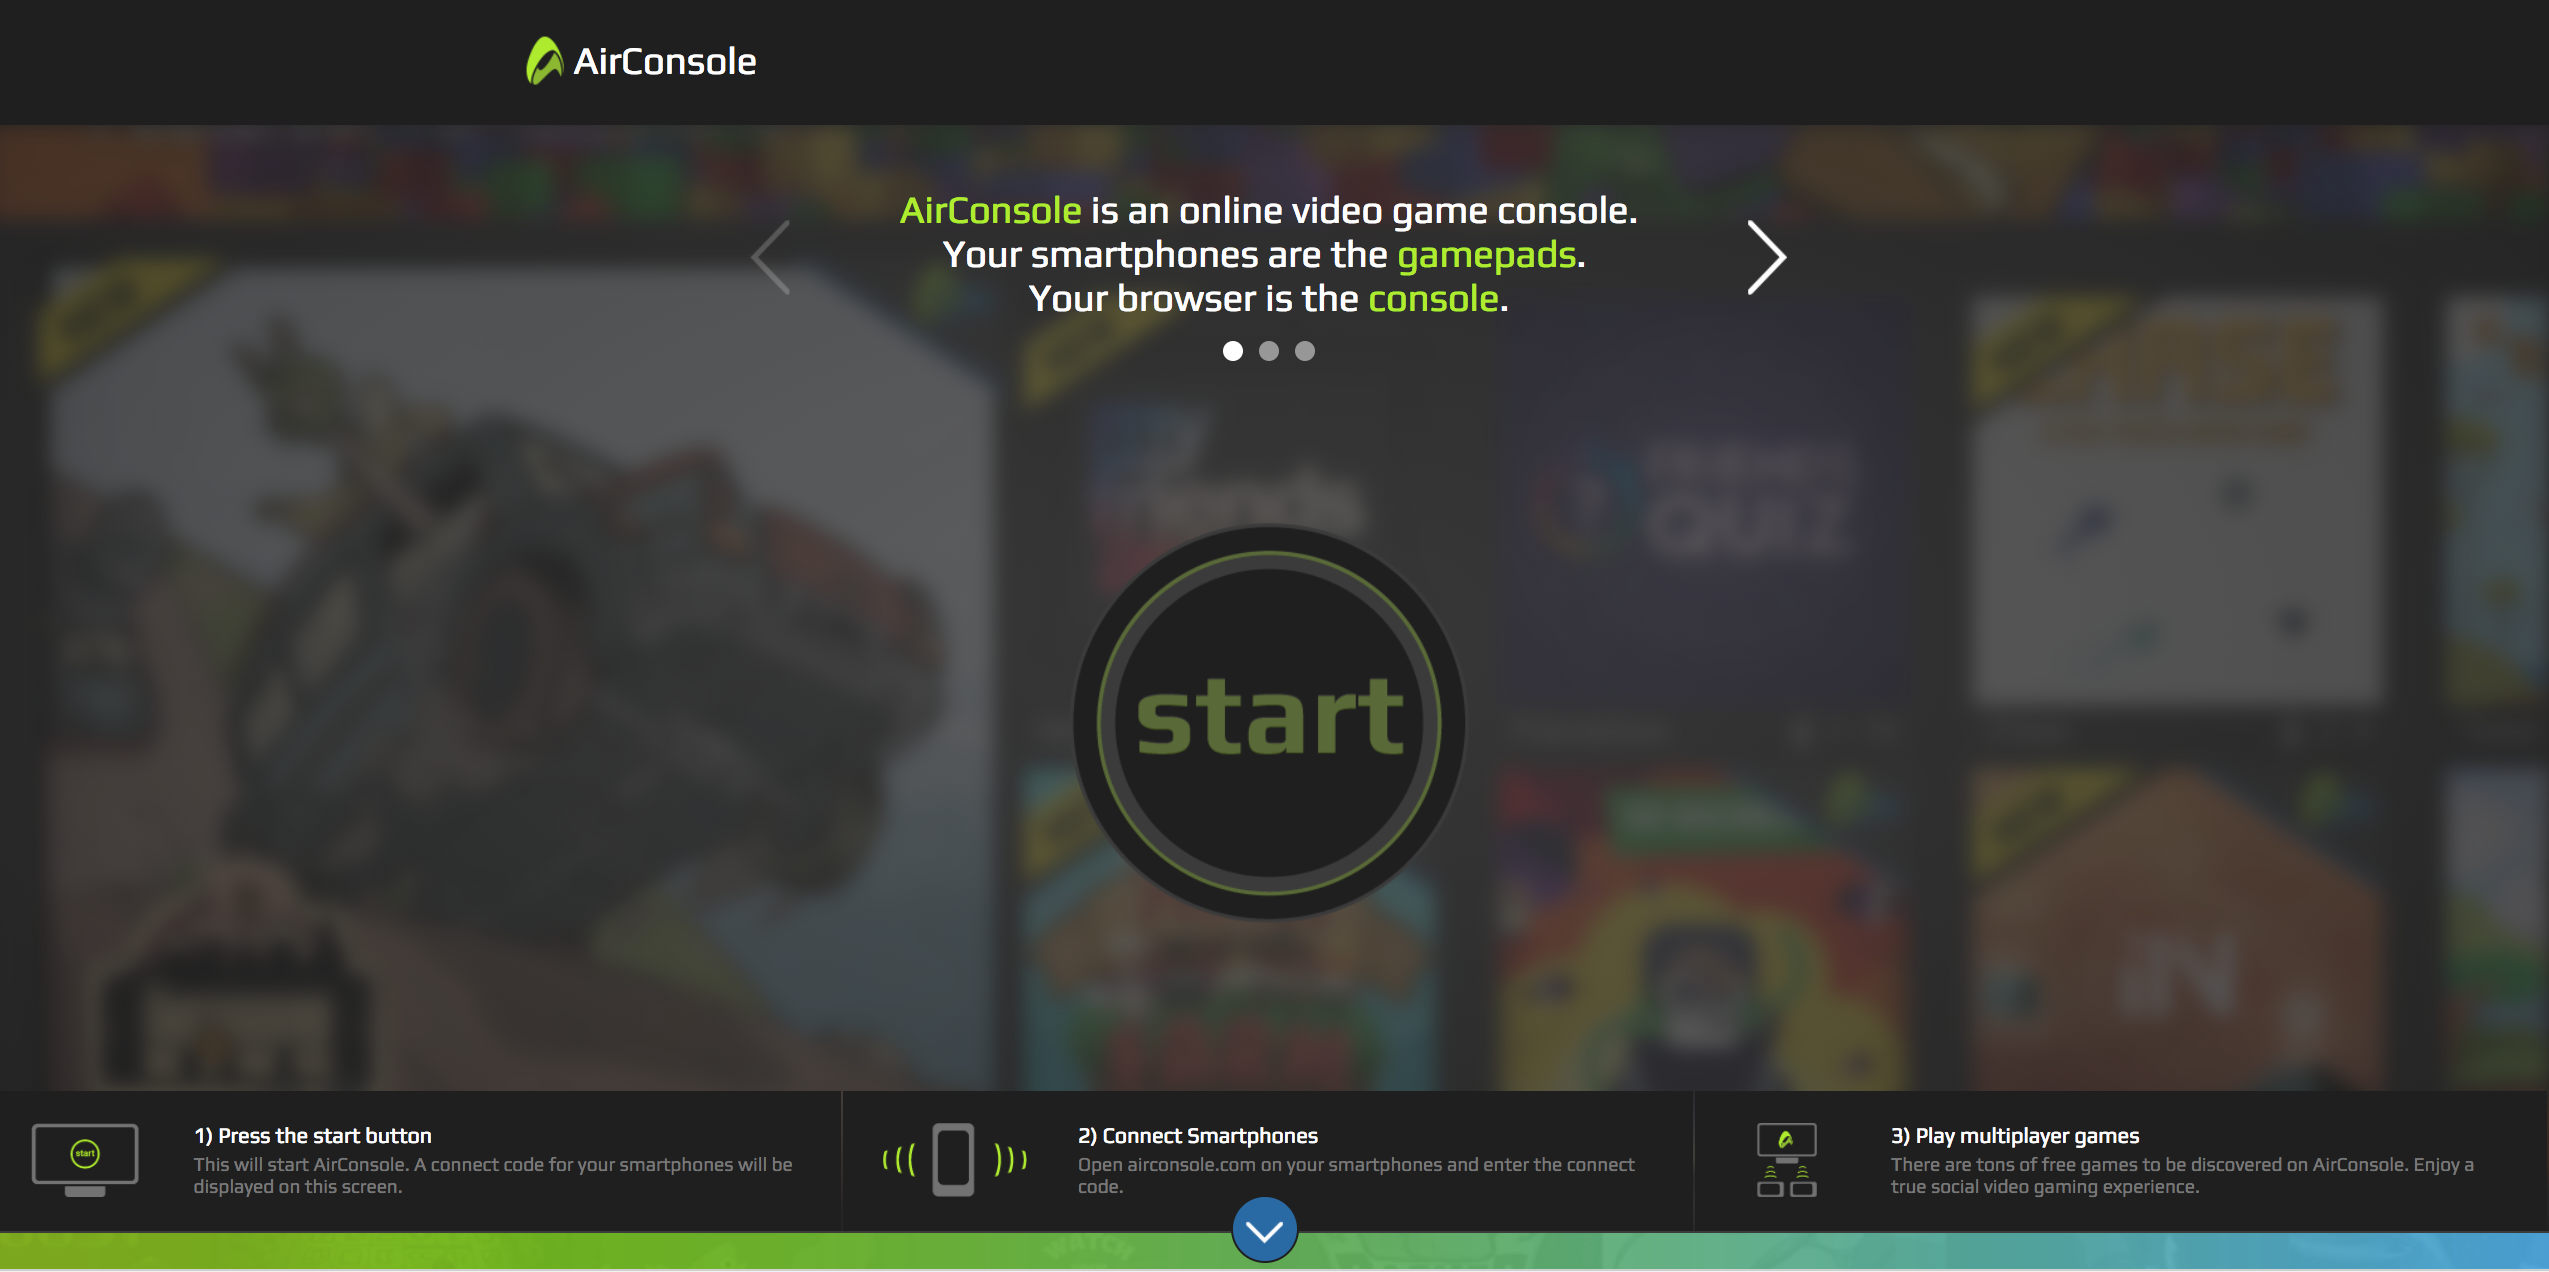
\includegraphics[scale=0.3]{Gambar/con1_home1}
			\caption{Halaman awal web pada \textit{PC browser}.}
			\label{fig:16_con1_home1}
		\end{figure}
	
		Setelah tombol \textit{start} ditekan, maka akan muncul halaman berikutnya yang menunjukan kode yang harus dimasukan oleh pemain pada \textit{mobile browser}. 
		
		\begin{figure}[H]
			\centering
			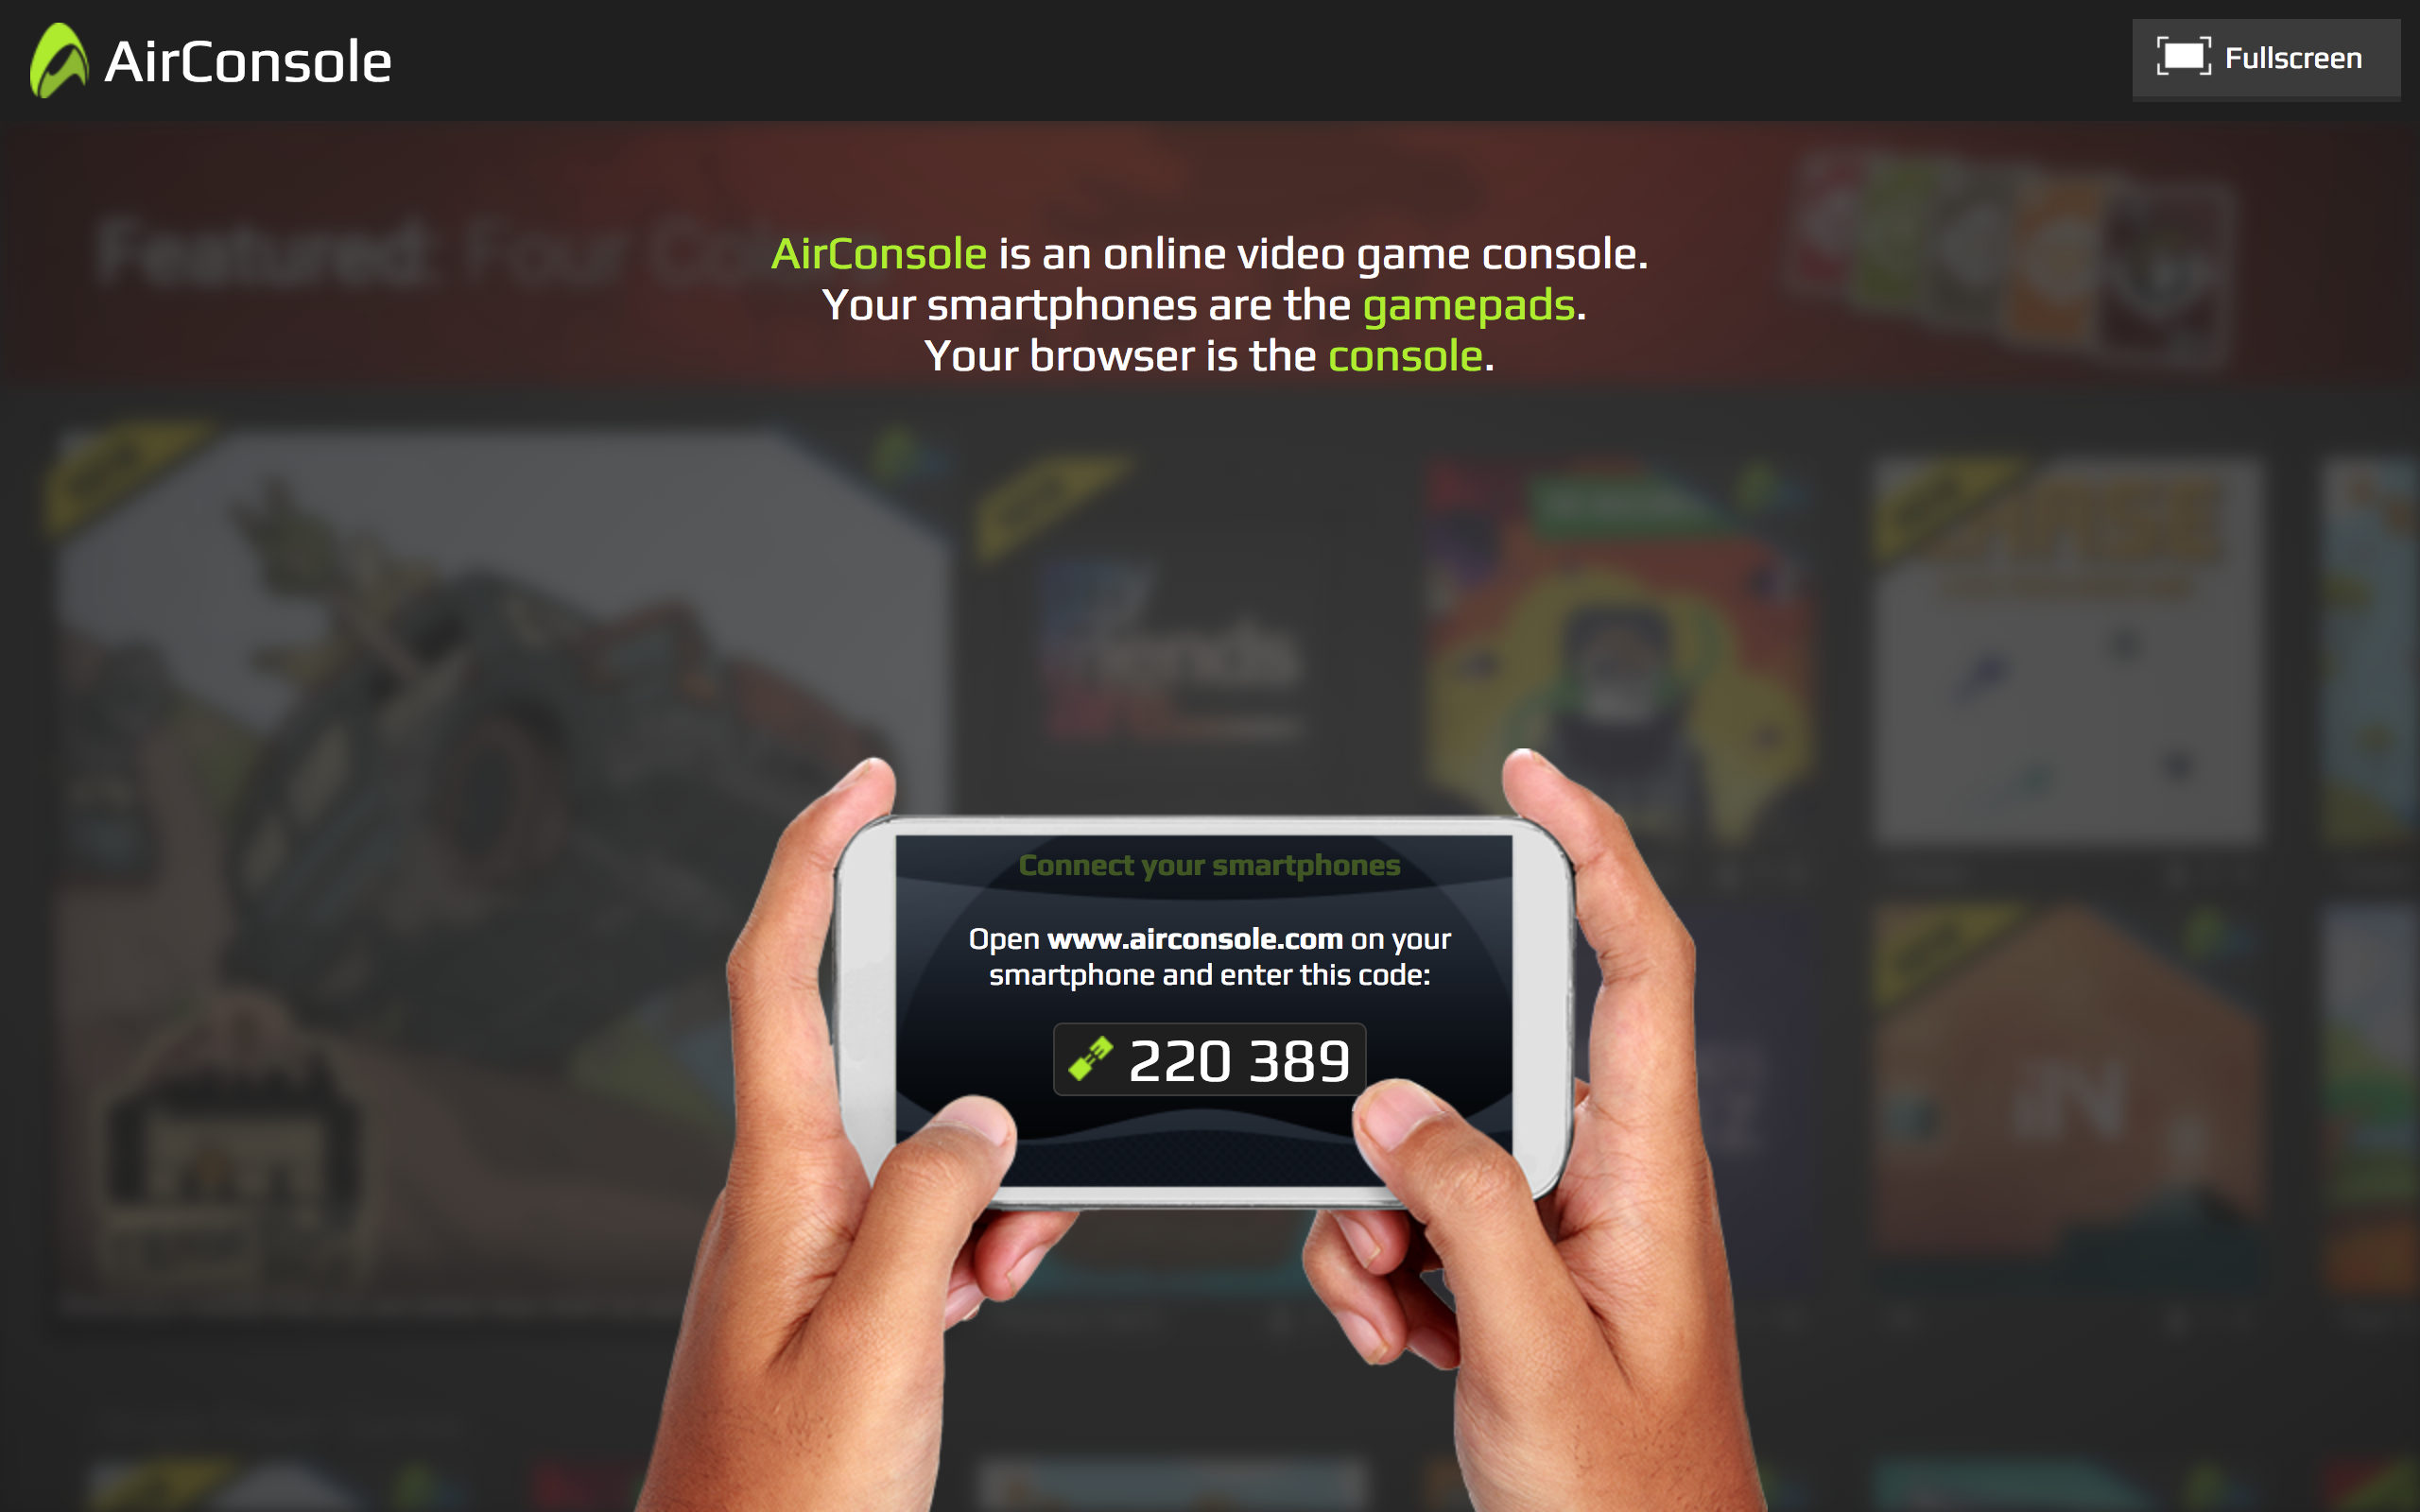
\includegraphics[scale=0.3]{Gambar/con2_code1}
			\caption{Kode yang harus dimasukan oleh pemain pada \textit{mobile browser}.}
			\label{fig:17_con2_code1}
		\end{figure}
		
		Pemain harus mengakses alamat web yang sama pada \textit{mobile browser}. Pada halaman awal, pemain akan diminta untuk memilih apakah akan bermain dengan menggunakan aplikasi, atau bermain dengan menggunakan \textit{browser}. 
		
		\begin{figure}[H]
			\centering
			
\includegraphics[scale=0.3]{Gambar/air1_home}
			\caption{Halaman awal pada \textit{mobile browser}.}
			\label{fig:18_air1_home}
		\end{figure}
	
		\vspace{-3cm}
		
		Dalam analisis ini, penulis memilih untuk bermain menggunakan \textit{browser}. Setelah itu, pemain diminta untuk menekan tombol \textit{'i got the connect code'} untuk memasukan kode yang sudah didapatkan pada \textit{PC browser}.
		
		\begin{figure}[H]
			\centering
			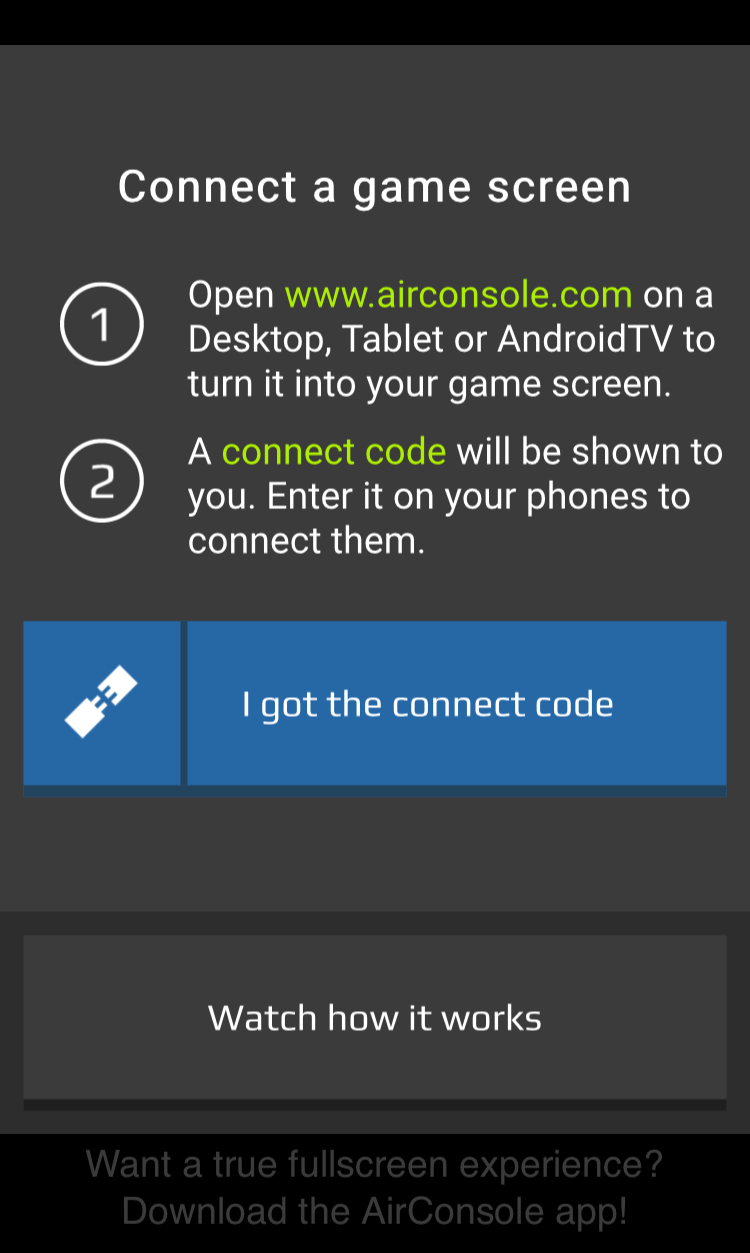
\includegraphics[scale=0.3]{Gambar/air2_code1}
			\caption{Pemain diminta untuk memasukan kode yang sudah didapatkan pada \textit{PC browser}.}
			\label{fig:19_air2_code1}
		\end{figure}
		
		
		Setelah menekan tombol tersebut, pemain dapat mulai memasukan kode yang sudah didapatkan. Kode ini bertujuan untuk proses otentikasi, sehingga para pemain yang dapat bermain dalam satu sesi yang sama, hanya para pemain yang mengetahui kode tersebut.
		
		\begin{figure}[H]
			
			\centering
			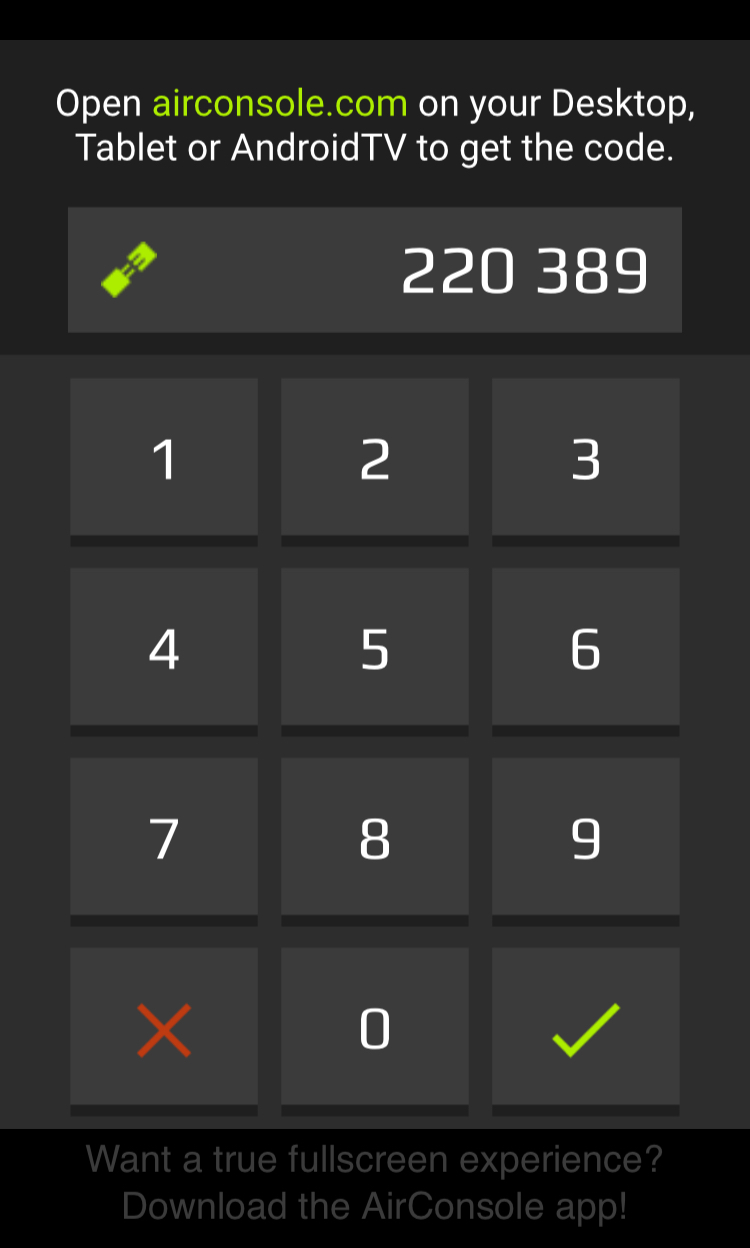
\includegraphics[scale=0.3]{Gambar/air3_code2}
			\caption{Pemain diminta untuk memasukan kode yang sudah didapatkan pada \textit{PC browser}.}
			\label{fig:20_air3_code2}
			
			
		\end{figure}
	
	
		Setelah pemain memasukan kode, maka halaman web di \textit{PC} dan \textit{smartphone} akan berubah. Pada \textit{PC}, halaman akan menunjukan berbagai jenis permainan yang dapat dipilih. Pada \textit{smartphone}, halaman akan berubah menjadi pengendali permainan, dimana pemain dapat menggerakan halaman yang ada di \textit{PC} dengan menggunakan \textit{smartphone}.
		
		\begin{figure}[H]
			\centering
			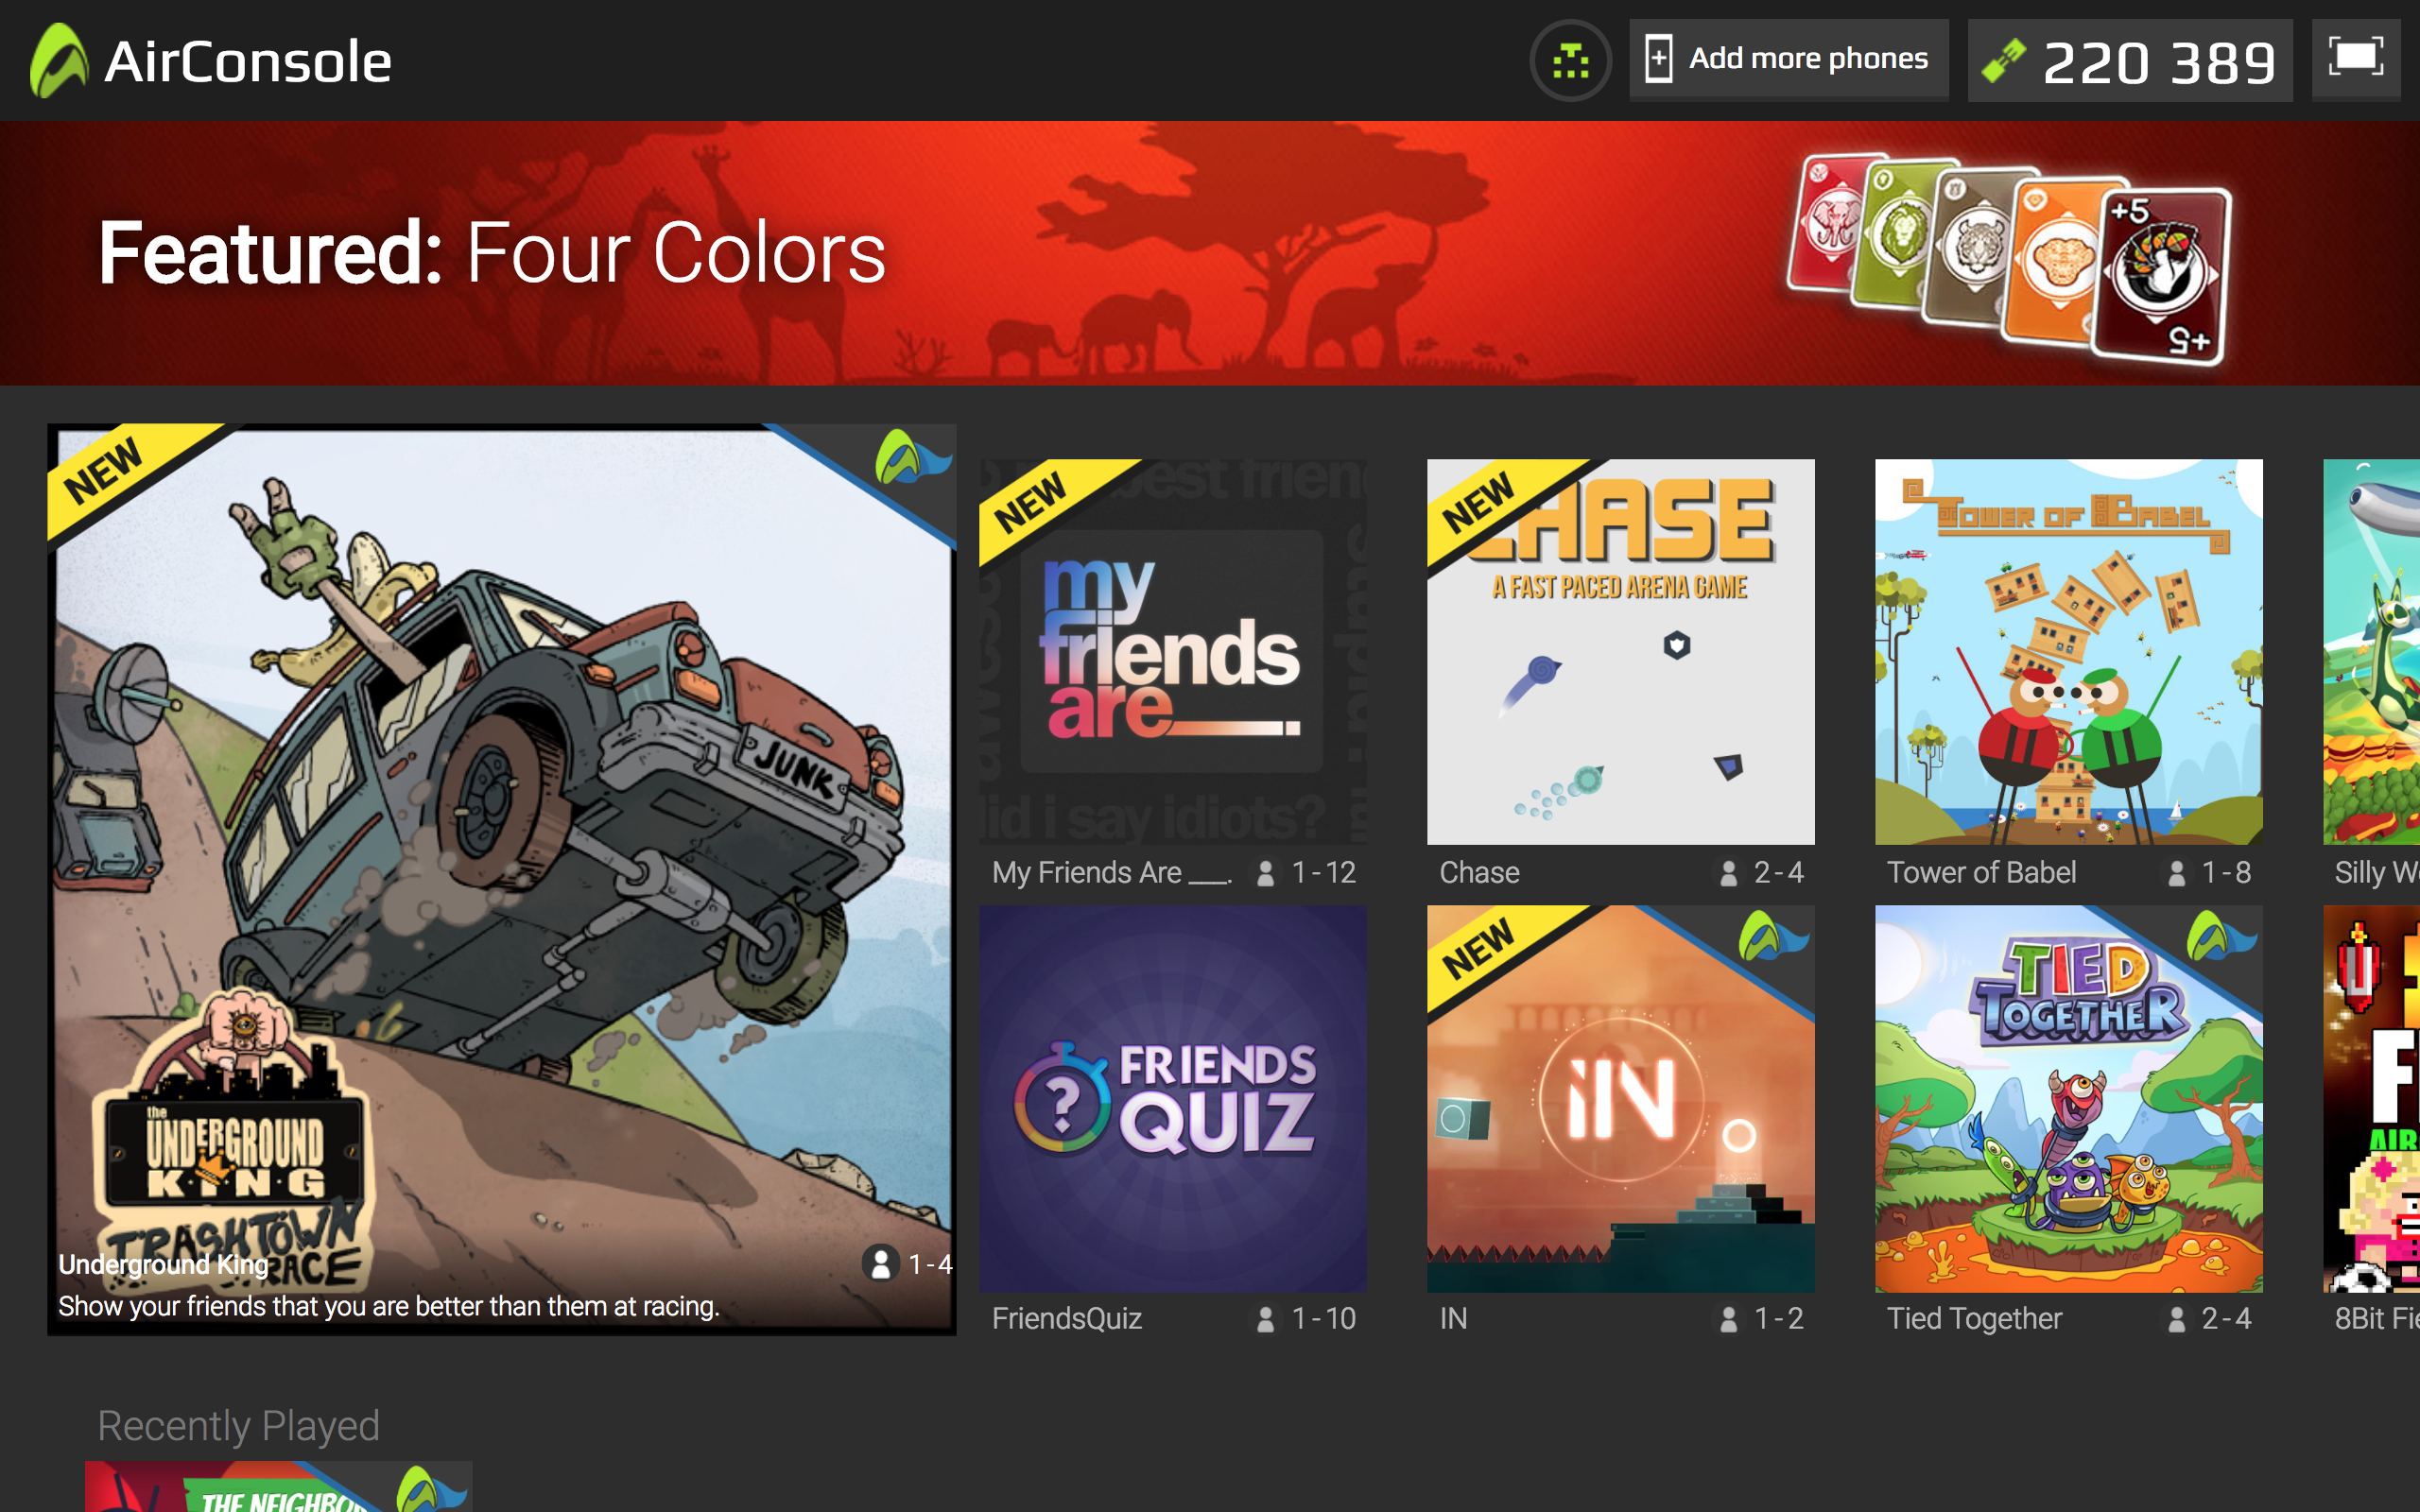
\includegraphics[scale=0.3]{Gambar/con3_play1}
			\caption{Halaman pada \textit{PC} yang menunjukan berbagai permainan yang dapat dipilih.}
			\label{fig:21_con3_play1}
		\end{figure}
	
		\begin{figure}[H]
			\centering
			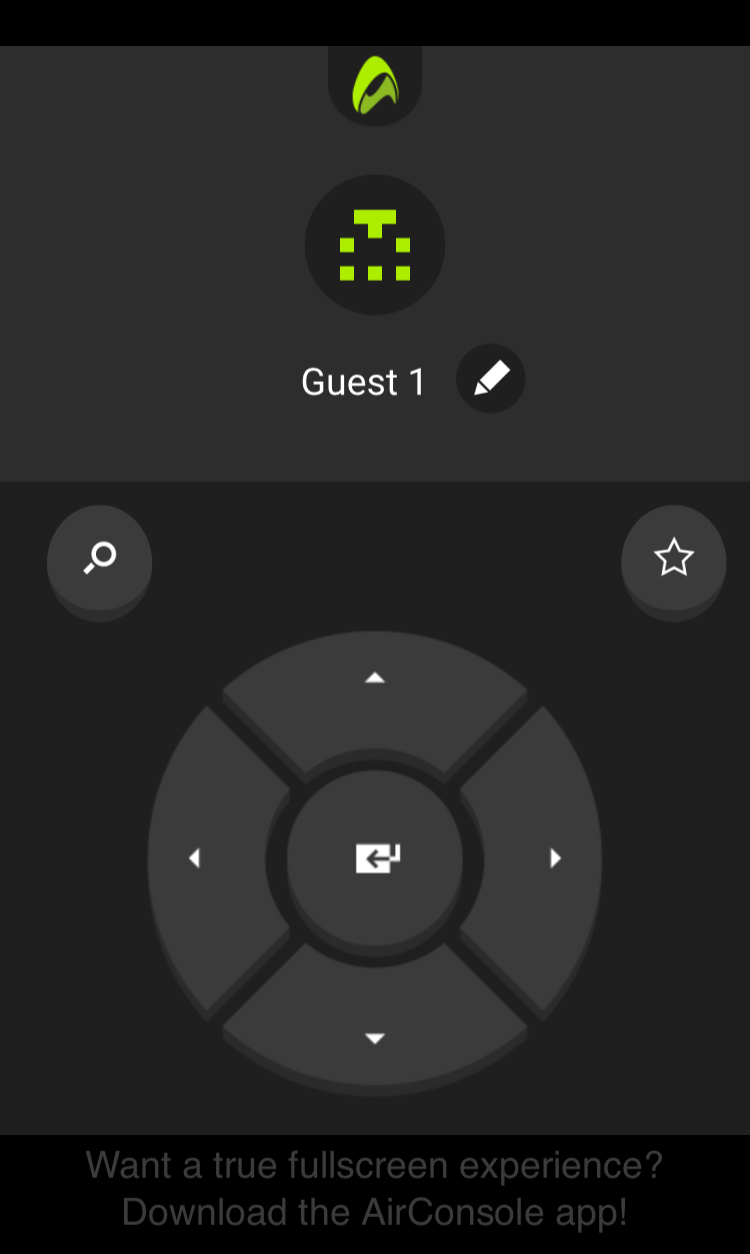
\includegraphics[scale=0.3]{Gambar/air4_play1}
			\caption{Halaman pada \textit{smartphone} yang berfungsi sebagai pengendali.}
			\label{fig:22_air4_play1}
		\end{figure}
		
		Dalam analisis ini, penulis memilih untuk memainkan permainan yang bernama The Neighborhood. Permainan ini sejenis permainan Angry Birds. Permainan ini bercerita tentang dua kelompok yang bertetangga, dimana kelompok tersebut bermusuhan dan berusaha untuk saling menghancurkan satu sama lain. Tujuan dari permainan ini yaitu lebih dulu menghancurkan anggota kelompok tetangga. Setelah memilih permainan tersebut, halaman pada \textit{PC} dan \textit{smartphone} akan berubah. Pada \textit{smartphone}, pemain akan diminta untuk merubah mode tampilan \textit{smartphone} menjadi \textit{landscape}.
		
		\begin{figure}[H]
			\centering
			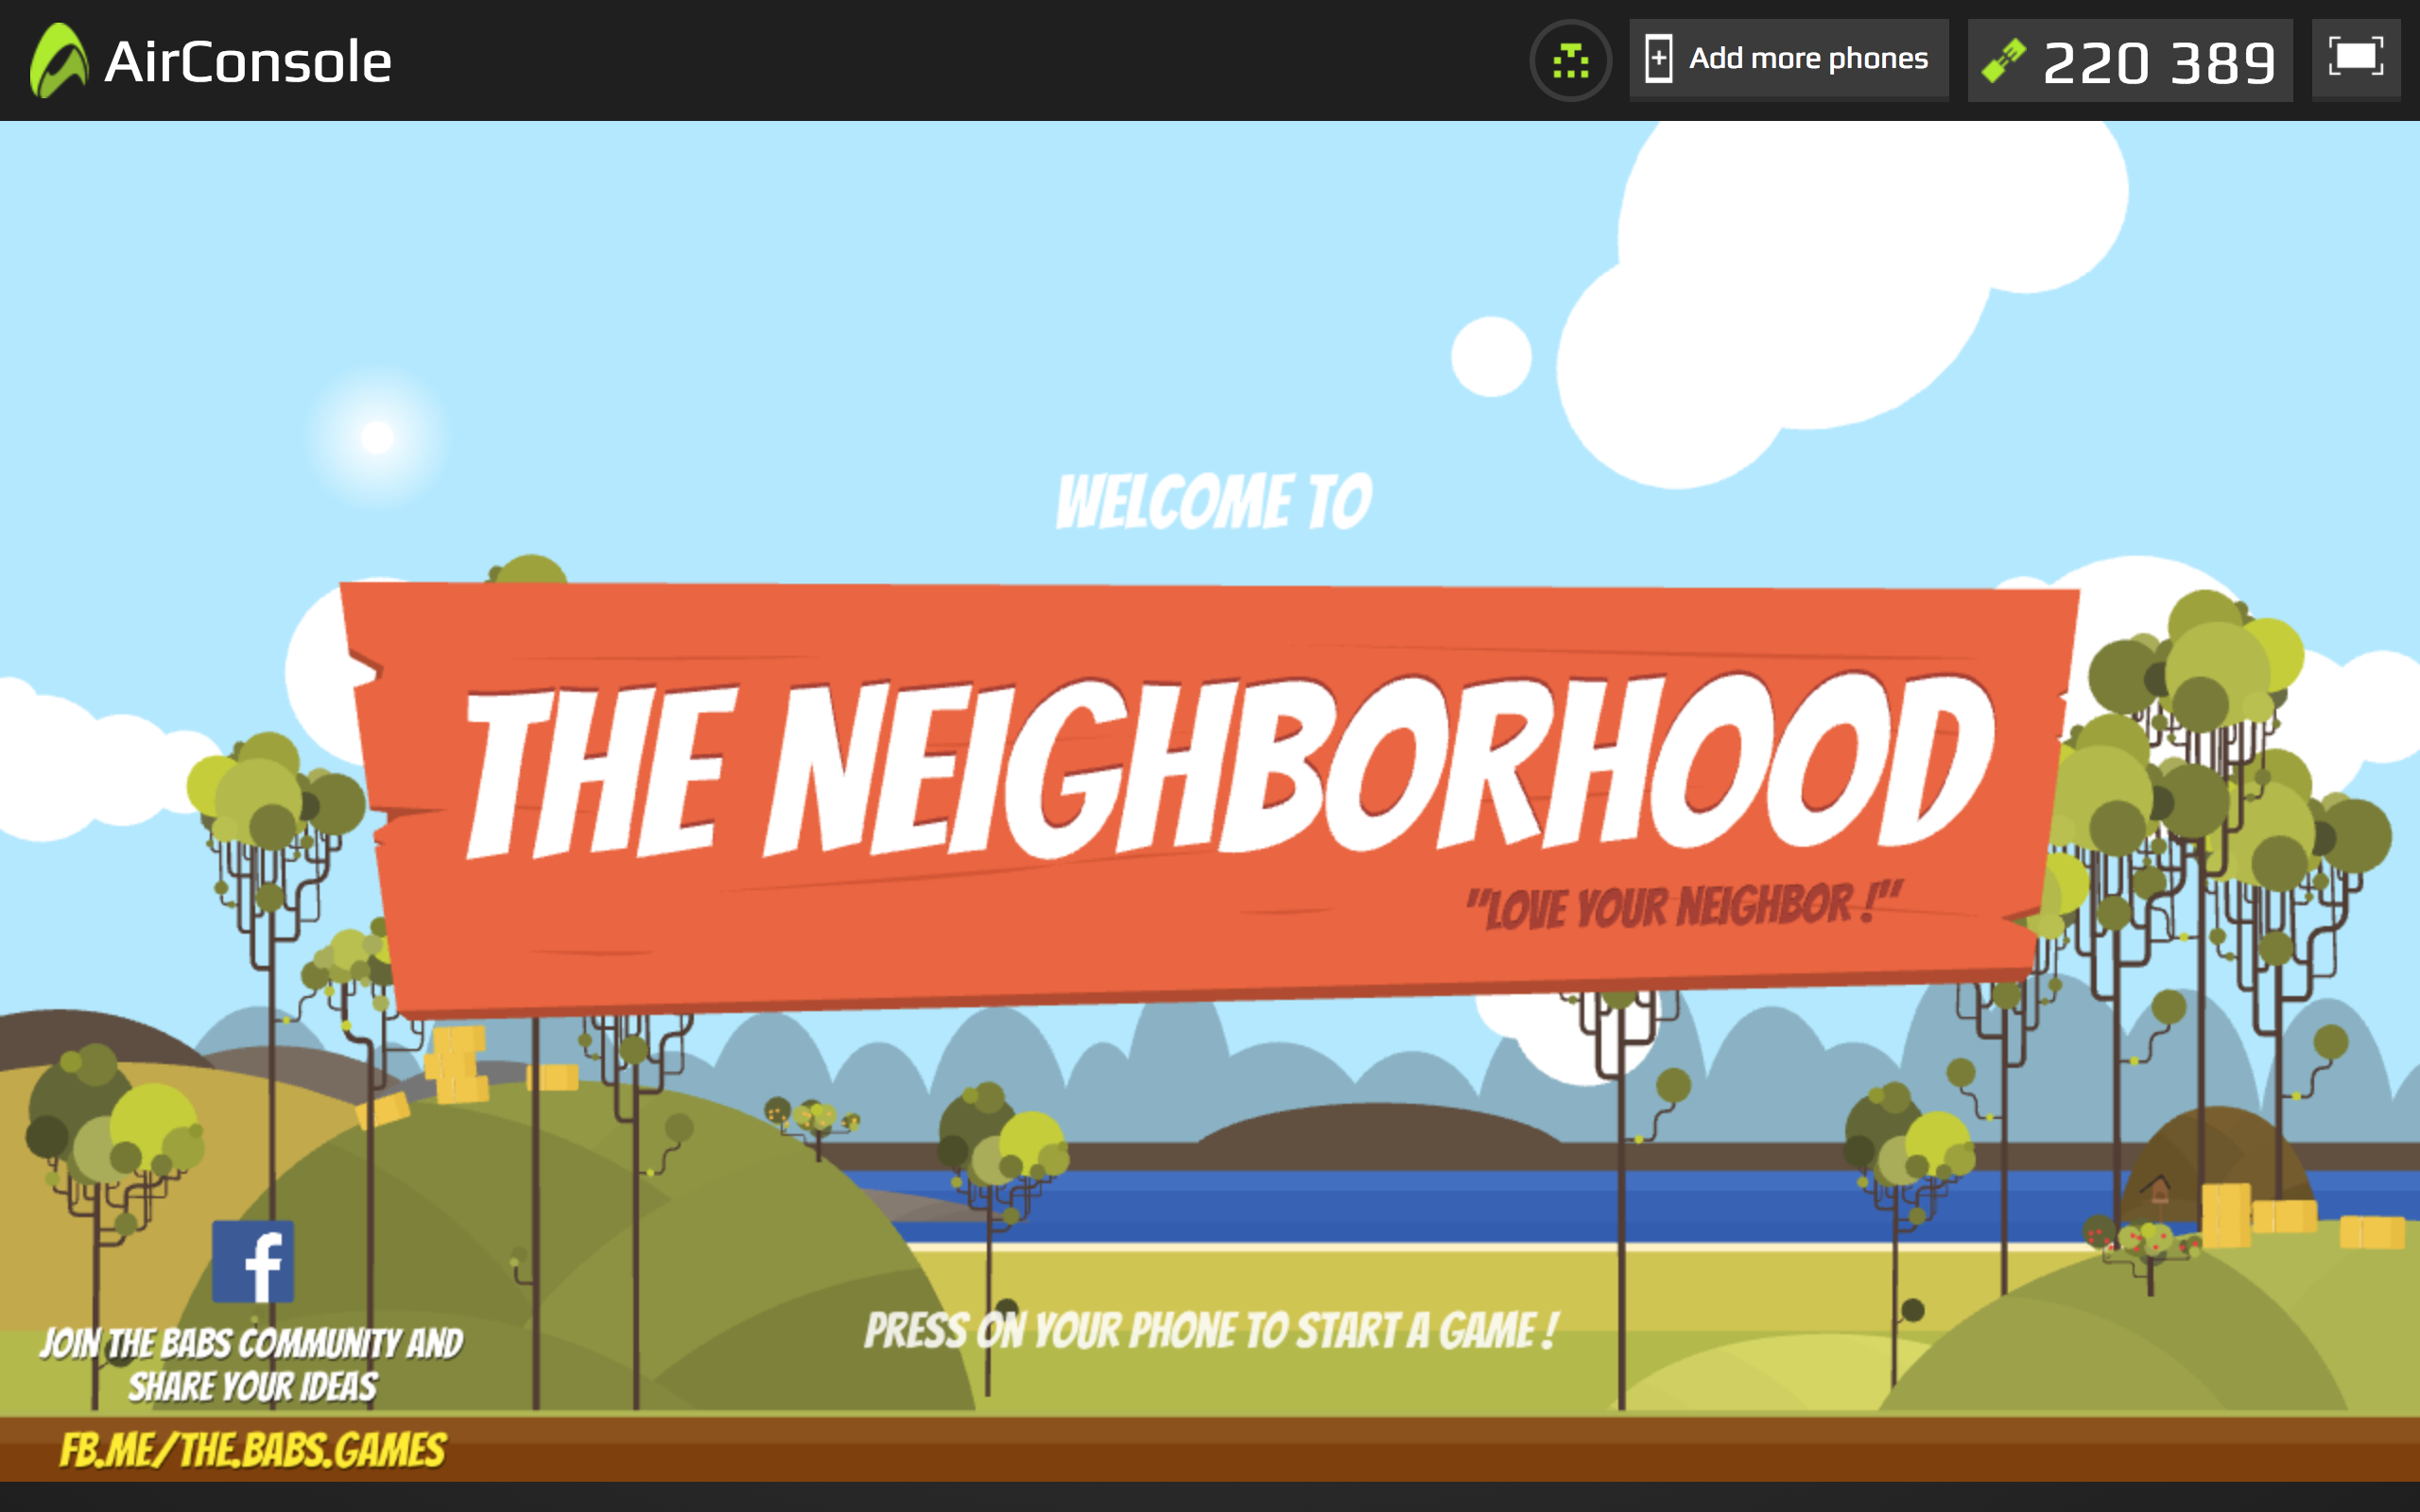
\includegraphics[scale=0.3]{Gambar/con5_play3}
			\caption{Halaman awal permainan The Neighborhood pada \textit{PC}.}
			\label{fig:23_con5_play3}
		\end{figure}
	
		\begin{figure}[H]
			\centering
			
\includegraphics[scale=0.3]{Gambar/air6_play3}
			\caption{Halaman awal permainan The Neighborhood pada \textit{smartphone}.}
			\label{fig:24_air6_play3}
		\end{figure}
		
		Cara bermain dari permainan tersebut yaitu dengan menggunakan \textit{smartphone}, dimana pemain harus menekan layar \textit{smartphone}, kemudian menariknya sesuai dengan arah yang berlawanan dengan lawan, lalu melepas jari dari layar \textit{smartphone} dengan tujuan untuk melempar suatu benda dari ketapel. Semakin jauh pemain menarik, maka lontaran benda tersebut akan semakin kencang mengenai lawan.
		
		\begin{figure}[H]
			\centering
			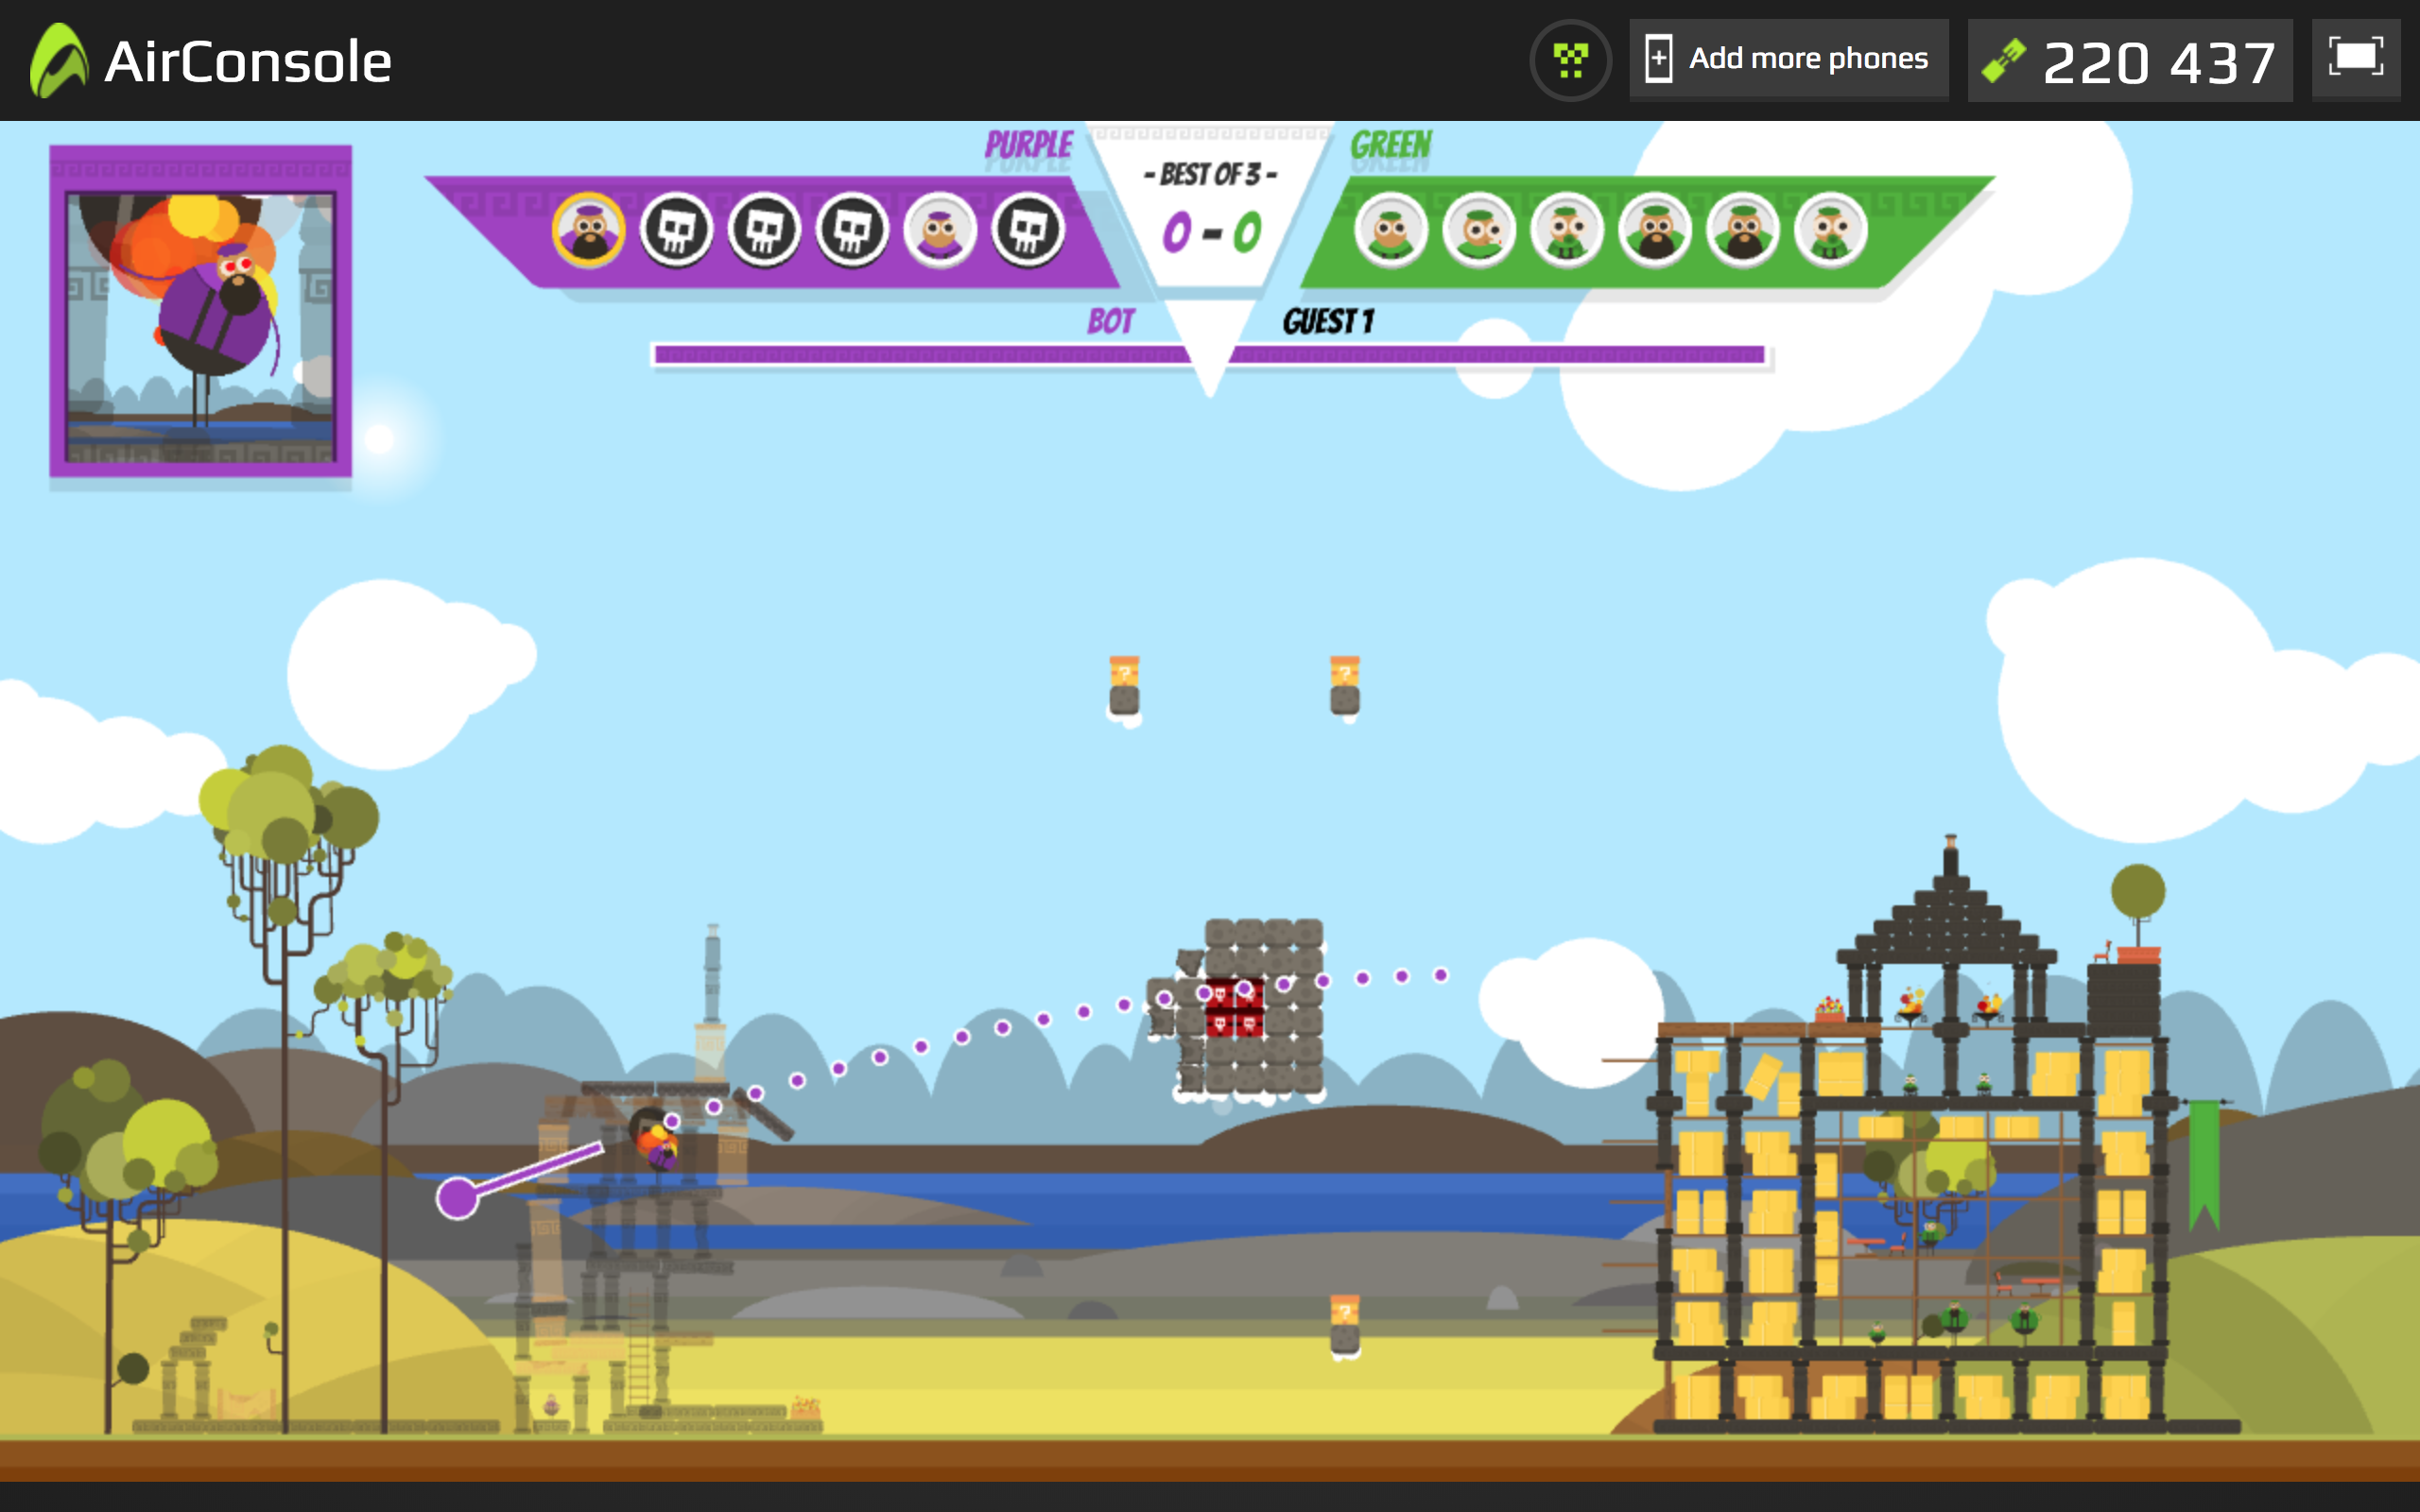
\includegraphics[scale=0.3]{Gambar/con7_play5}
			\caption{Halaman pada \textit{PC} dimana permainan sedang berlangsung.}
			\label{fig:25_con7_play5}
		\end{figure}
	
		\begin{figure}[H]
			\centering
			
\includegraphics[scale=0.3]{Gambar/air7_play4}
			\caption{Halaman pada \textit{smartphone} dimana permainan sedang berlangsung.}
			\label{fig:26_air7_play4}
		\end{figure}
	
		Apabila memenangkan permainan tersebut, maka pemain dapat memilih untuk keluar dari permainan atau melanjutkan permainannya kembali.
		
		\begin{figure}[H]
			\centering
			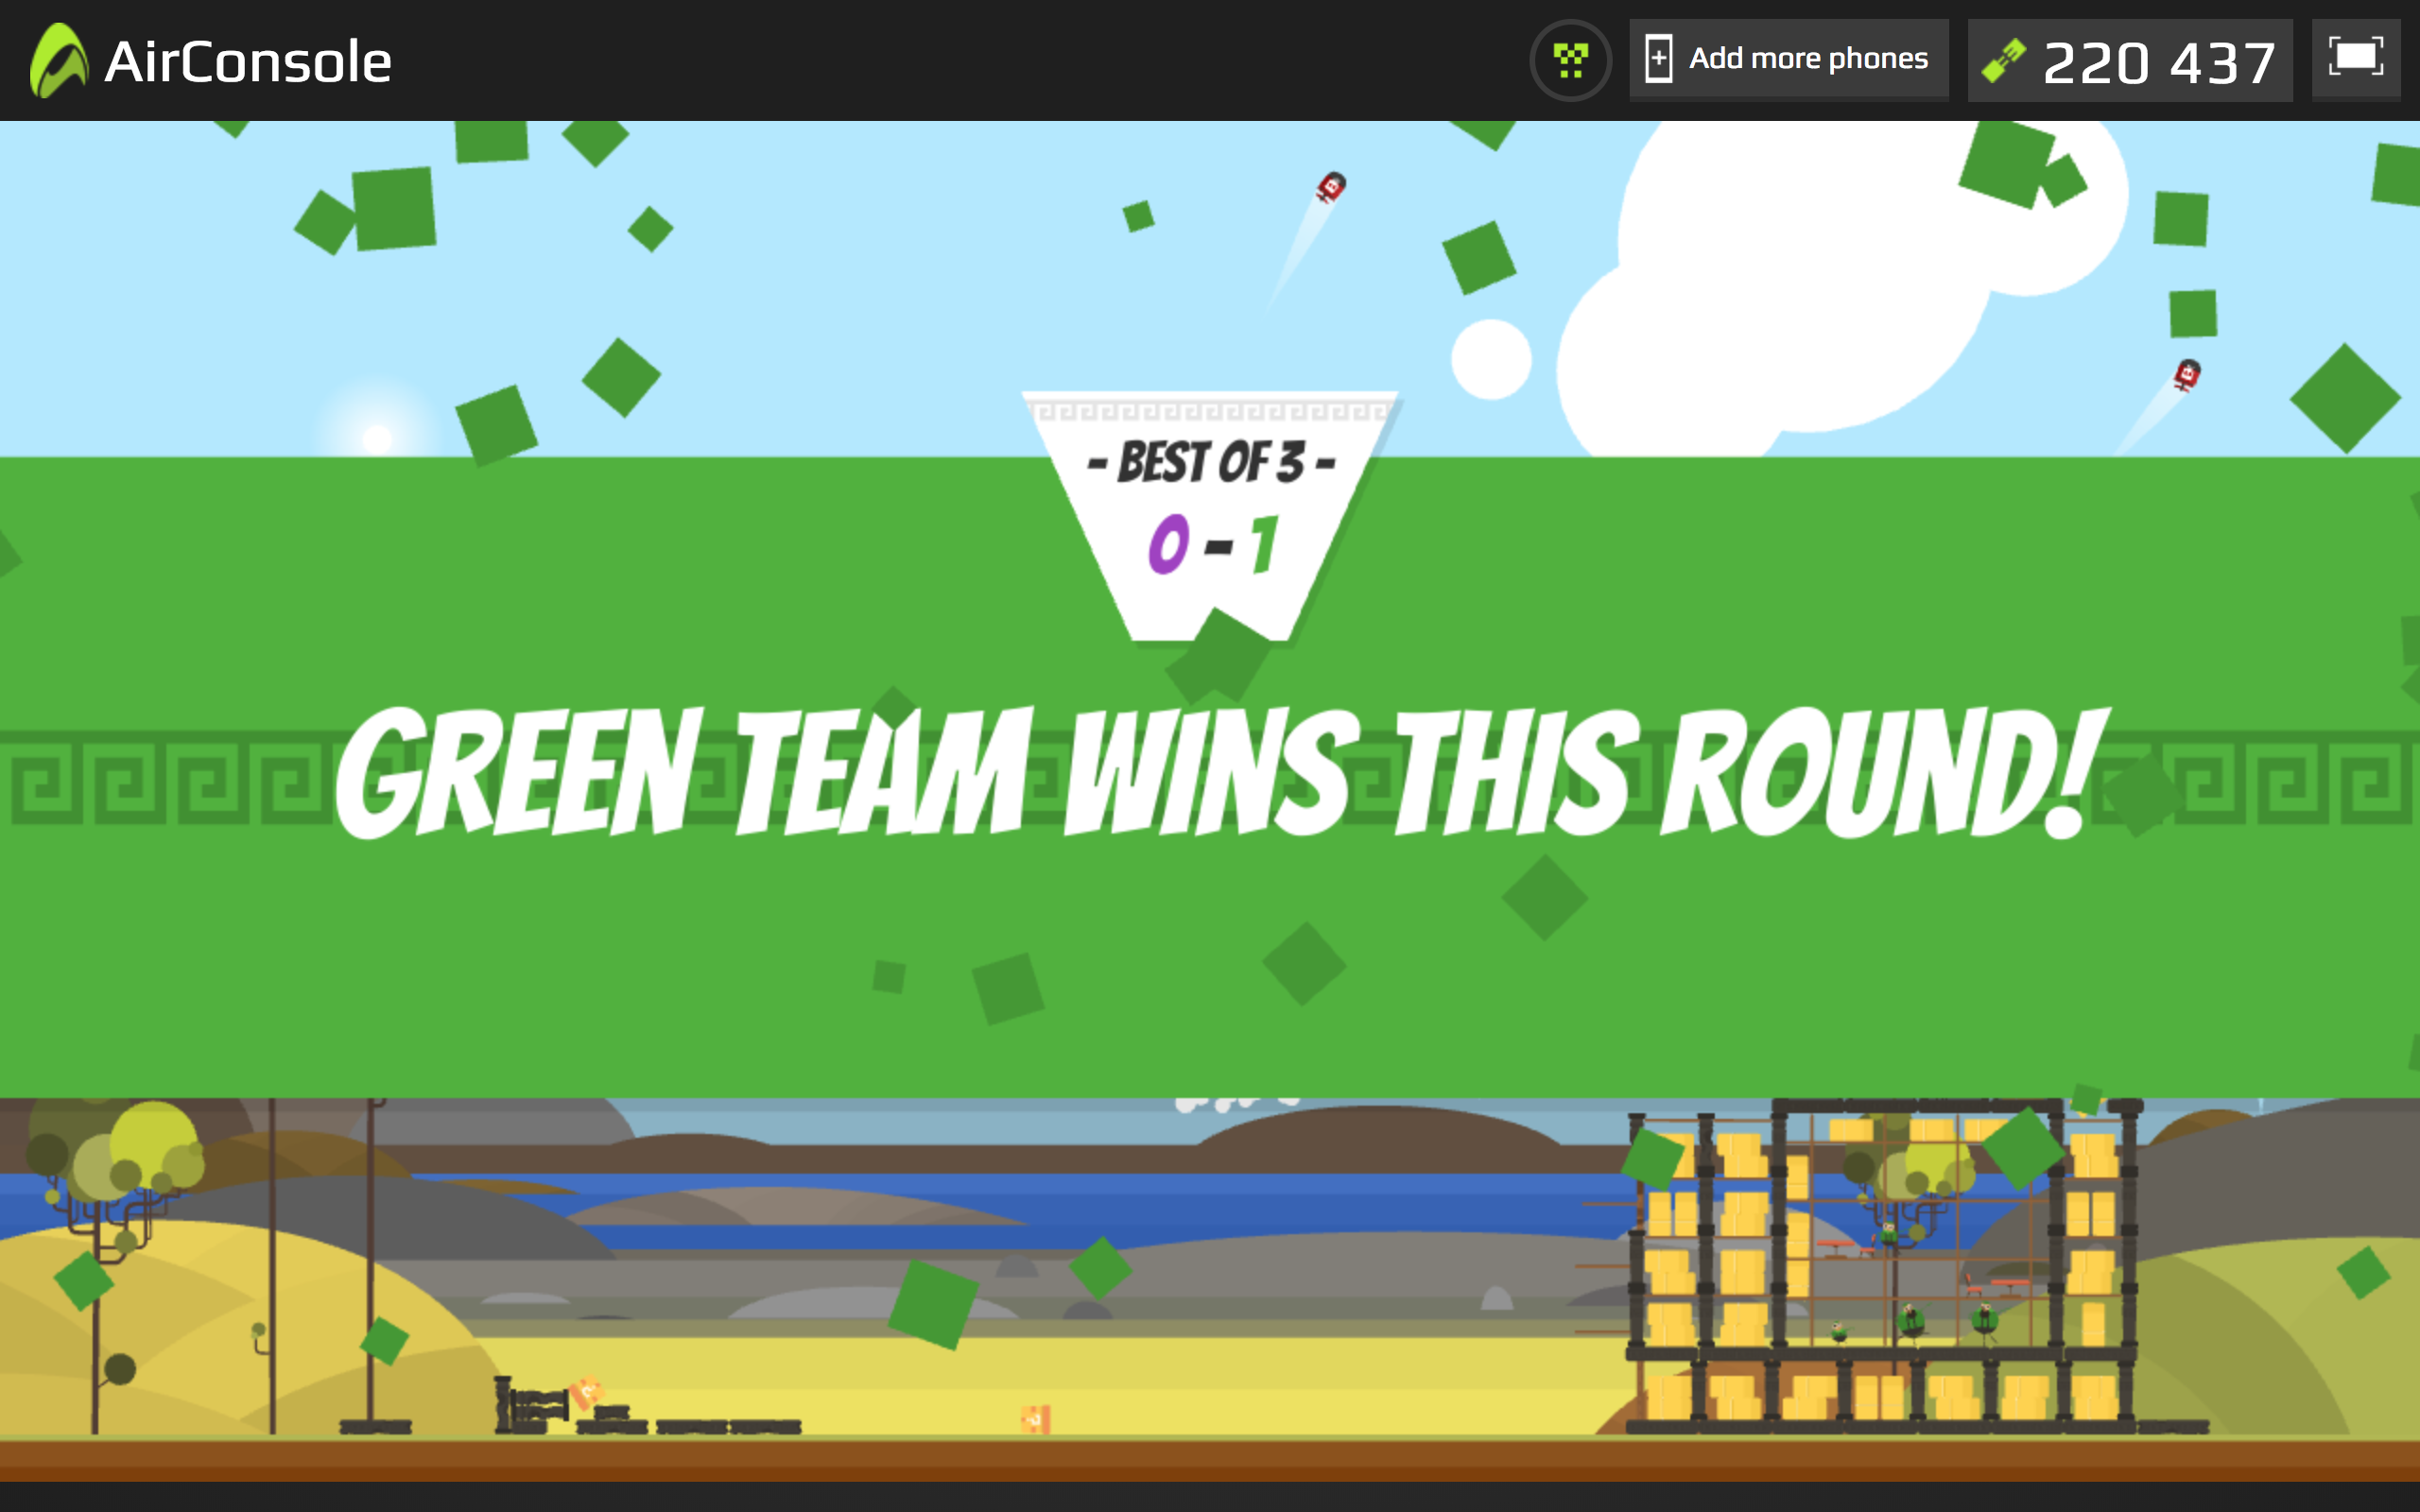
\includegraphics[scale=0.3]{Gambar/con8_play6}
			\caption{Halaman pada \textit{PC} apabila permainan sudah dimenangkan.}
			\label{fig:27_con8_play6}
		\end{figure}
	
		\begin{figure}[H]
			\centering
			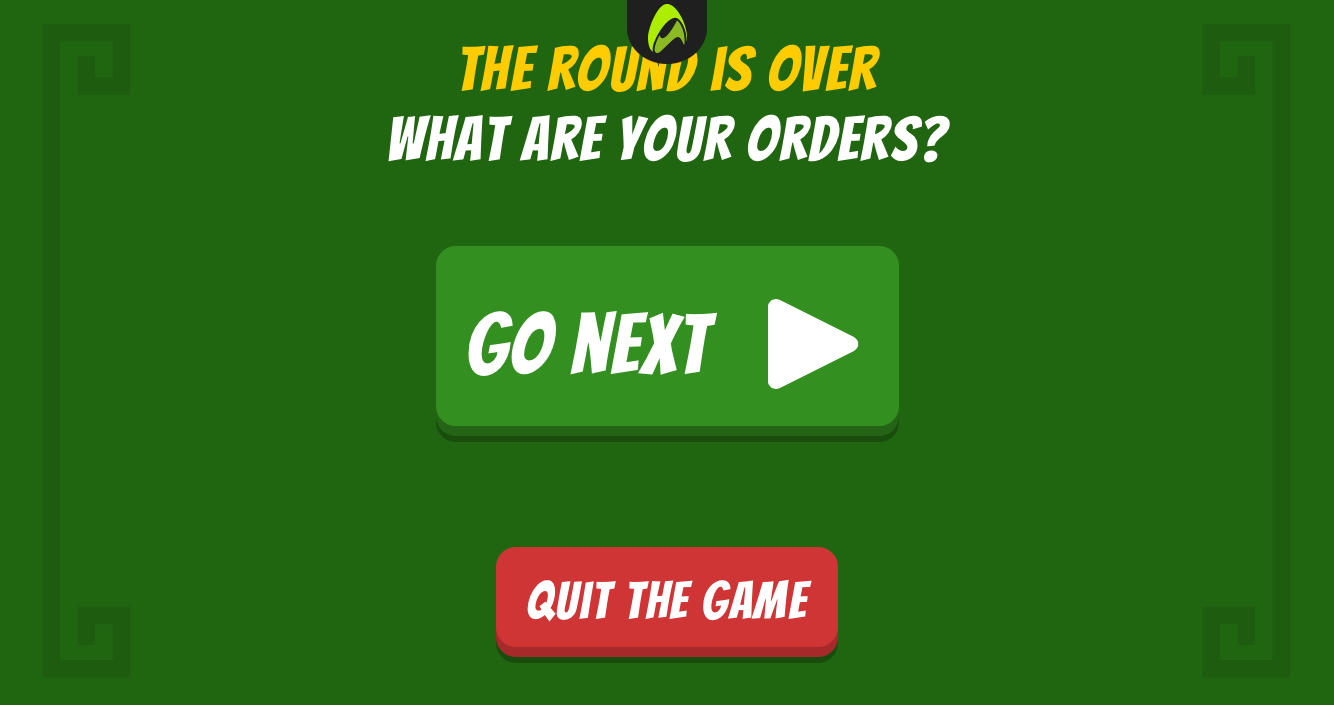
\includegraphics[scale=0.3]{Gambar/air8_finish}
			\caption{Halaman pada \textit{smartphone} apabila permainan sudah dimenangkan.}
			\label{fig:28_air8_finish}
		\end{figure}
	
		Dari ketiga percobaan yang sudah dilakukan, ada beberapa hal yang dapat diperbaiki dari permainan berbasis web tersebut. Percobaan pertama menunjukan hasil yang bagus, dimana koneksi antara \textit{smartphone} dan \textit{PC} tidak putus saat permainan berlangsung, dan juga tidak ada keterlambatan antara gerakan pada \textit{smartphone} dan \textit{PC}. Pada percobaan kedua, apabila \textit{browser} pada \textit{PC} ditutup pada saat permainan berlangsung, maka koneksi akan terputus. Tetapi, tampilan pada \textit{smartphone} tidak menunjukan bahwa adanya koneksi yang terputus, sehingga pemain tidak mengetahui apakah permainan masih dapat berlangsung atau tidak. Tampilan hanya akan langsung kembali pada halaman awal permainan. Begitupun dengan percobaan ketiga, apabila \textit{browser} pada \textit{smartphone} ditutup pada saat permainan sedang berlangsung, maka koneksi akan terputus. Tampilan pada \textit{PC} hanya menunjukan tanda kecil bahwa telah terjadi pemutusan koneksi pada \textit{smartphone}, yaitu tanda x pada bagian atas tampilan yang ditunjukan seperti gambar berikut:
		
		\begin{figure}[H]
			\centering
			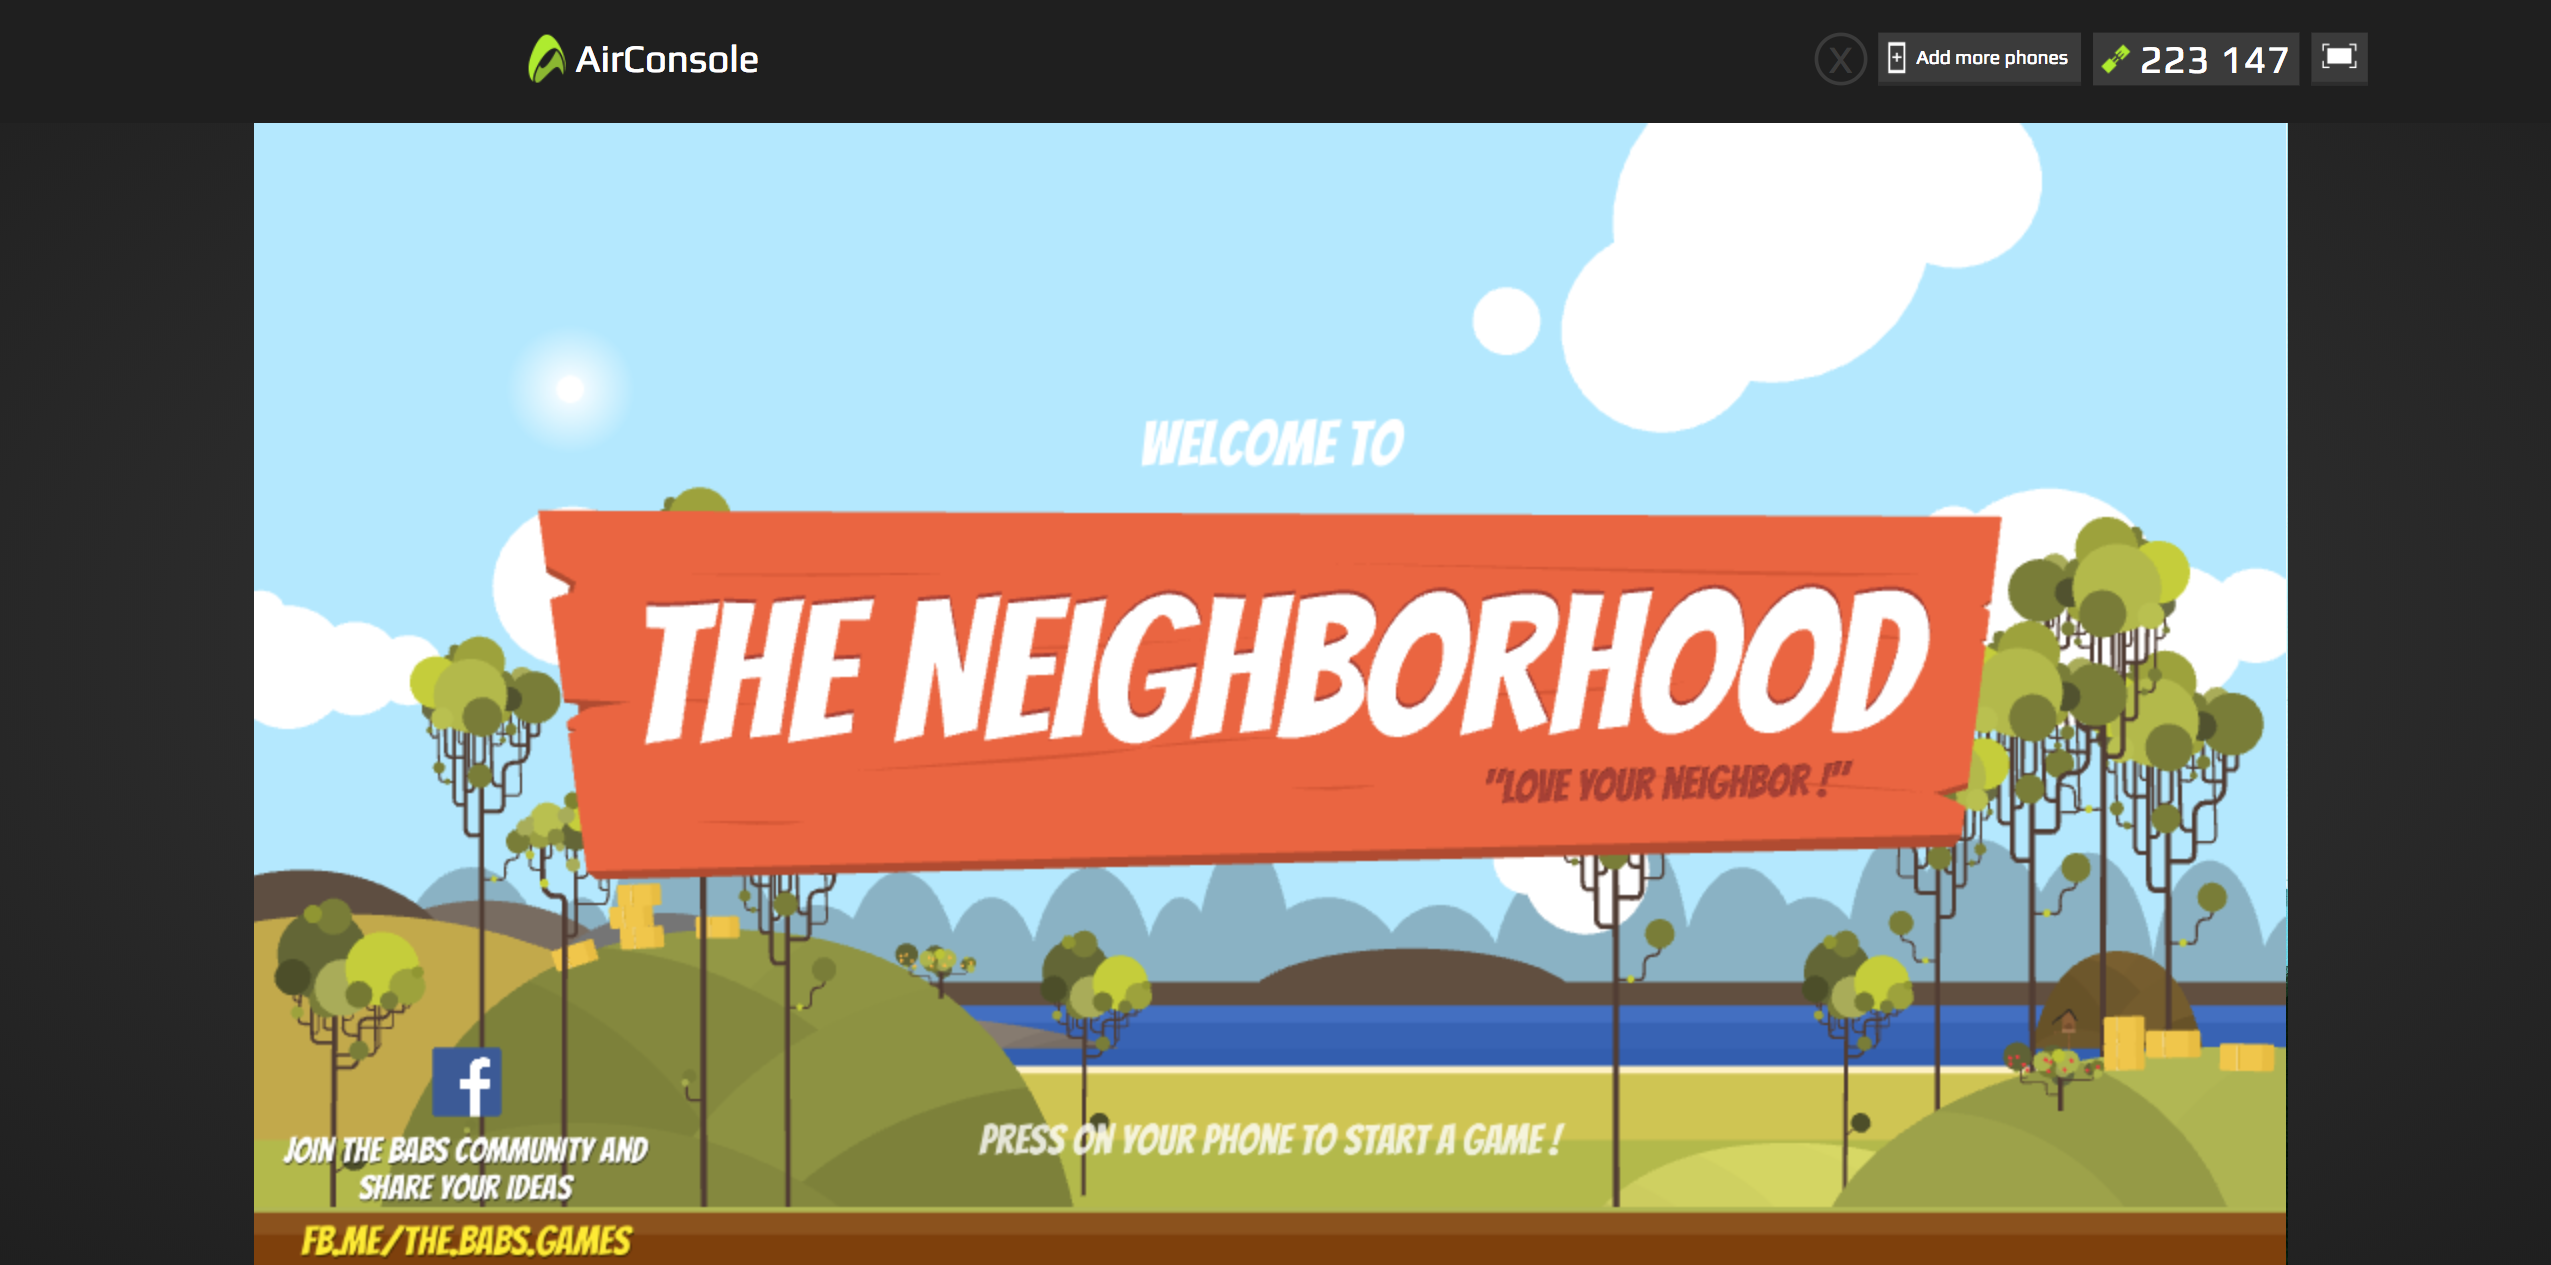
\includegraphics[scale=0.3]{Gambar/con9_play7}
			\caption{Halaman pada \textit{PC} yang menunjukan pemutusan koneksi.}
			\label{fig:29_con9_play7}
		\end{figure}
		
		Perbaikan yang dapat dilakukan adalah dengan memberi \textit{feedback} yang lebih jelas pada pemain, apabila ada kesalahan pada aplikasi yang terjadi seperti pemutusan koneksi. Dengan begitu, pemain akan lebih mengetahui bahwa koneksi dapat saja terputus dan tidak dapat melanjutkan permainannya.
		
		\item Merancang antarmuka permainan pada \textit{PC} dan \textit{smartphone}.\\
		{\bf status :} Ada sejak rencana kerja skripsi.\\
		{\bf hasil :} \\
		
		Antarmuka yang dirancang terbagi menjadi dua bagian, yaitu antarmuka pada \textit{browser} yang ada di \textit{PC} dan \textit{smartphone}.
		
		\textbf{PC}
		
		\begin{figure}[H]
			\centering
			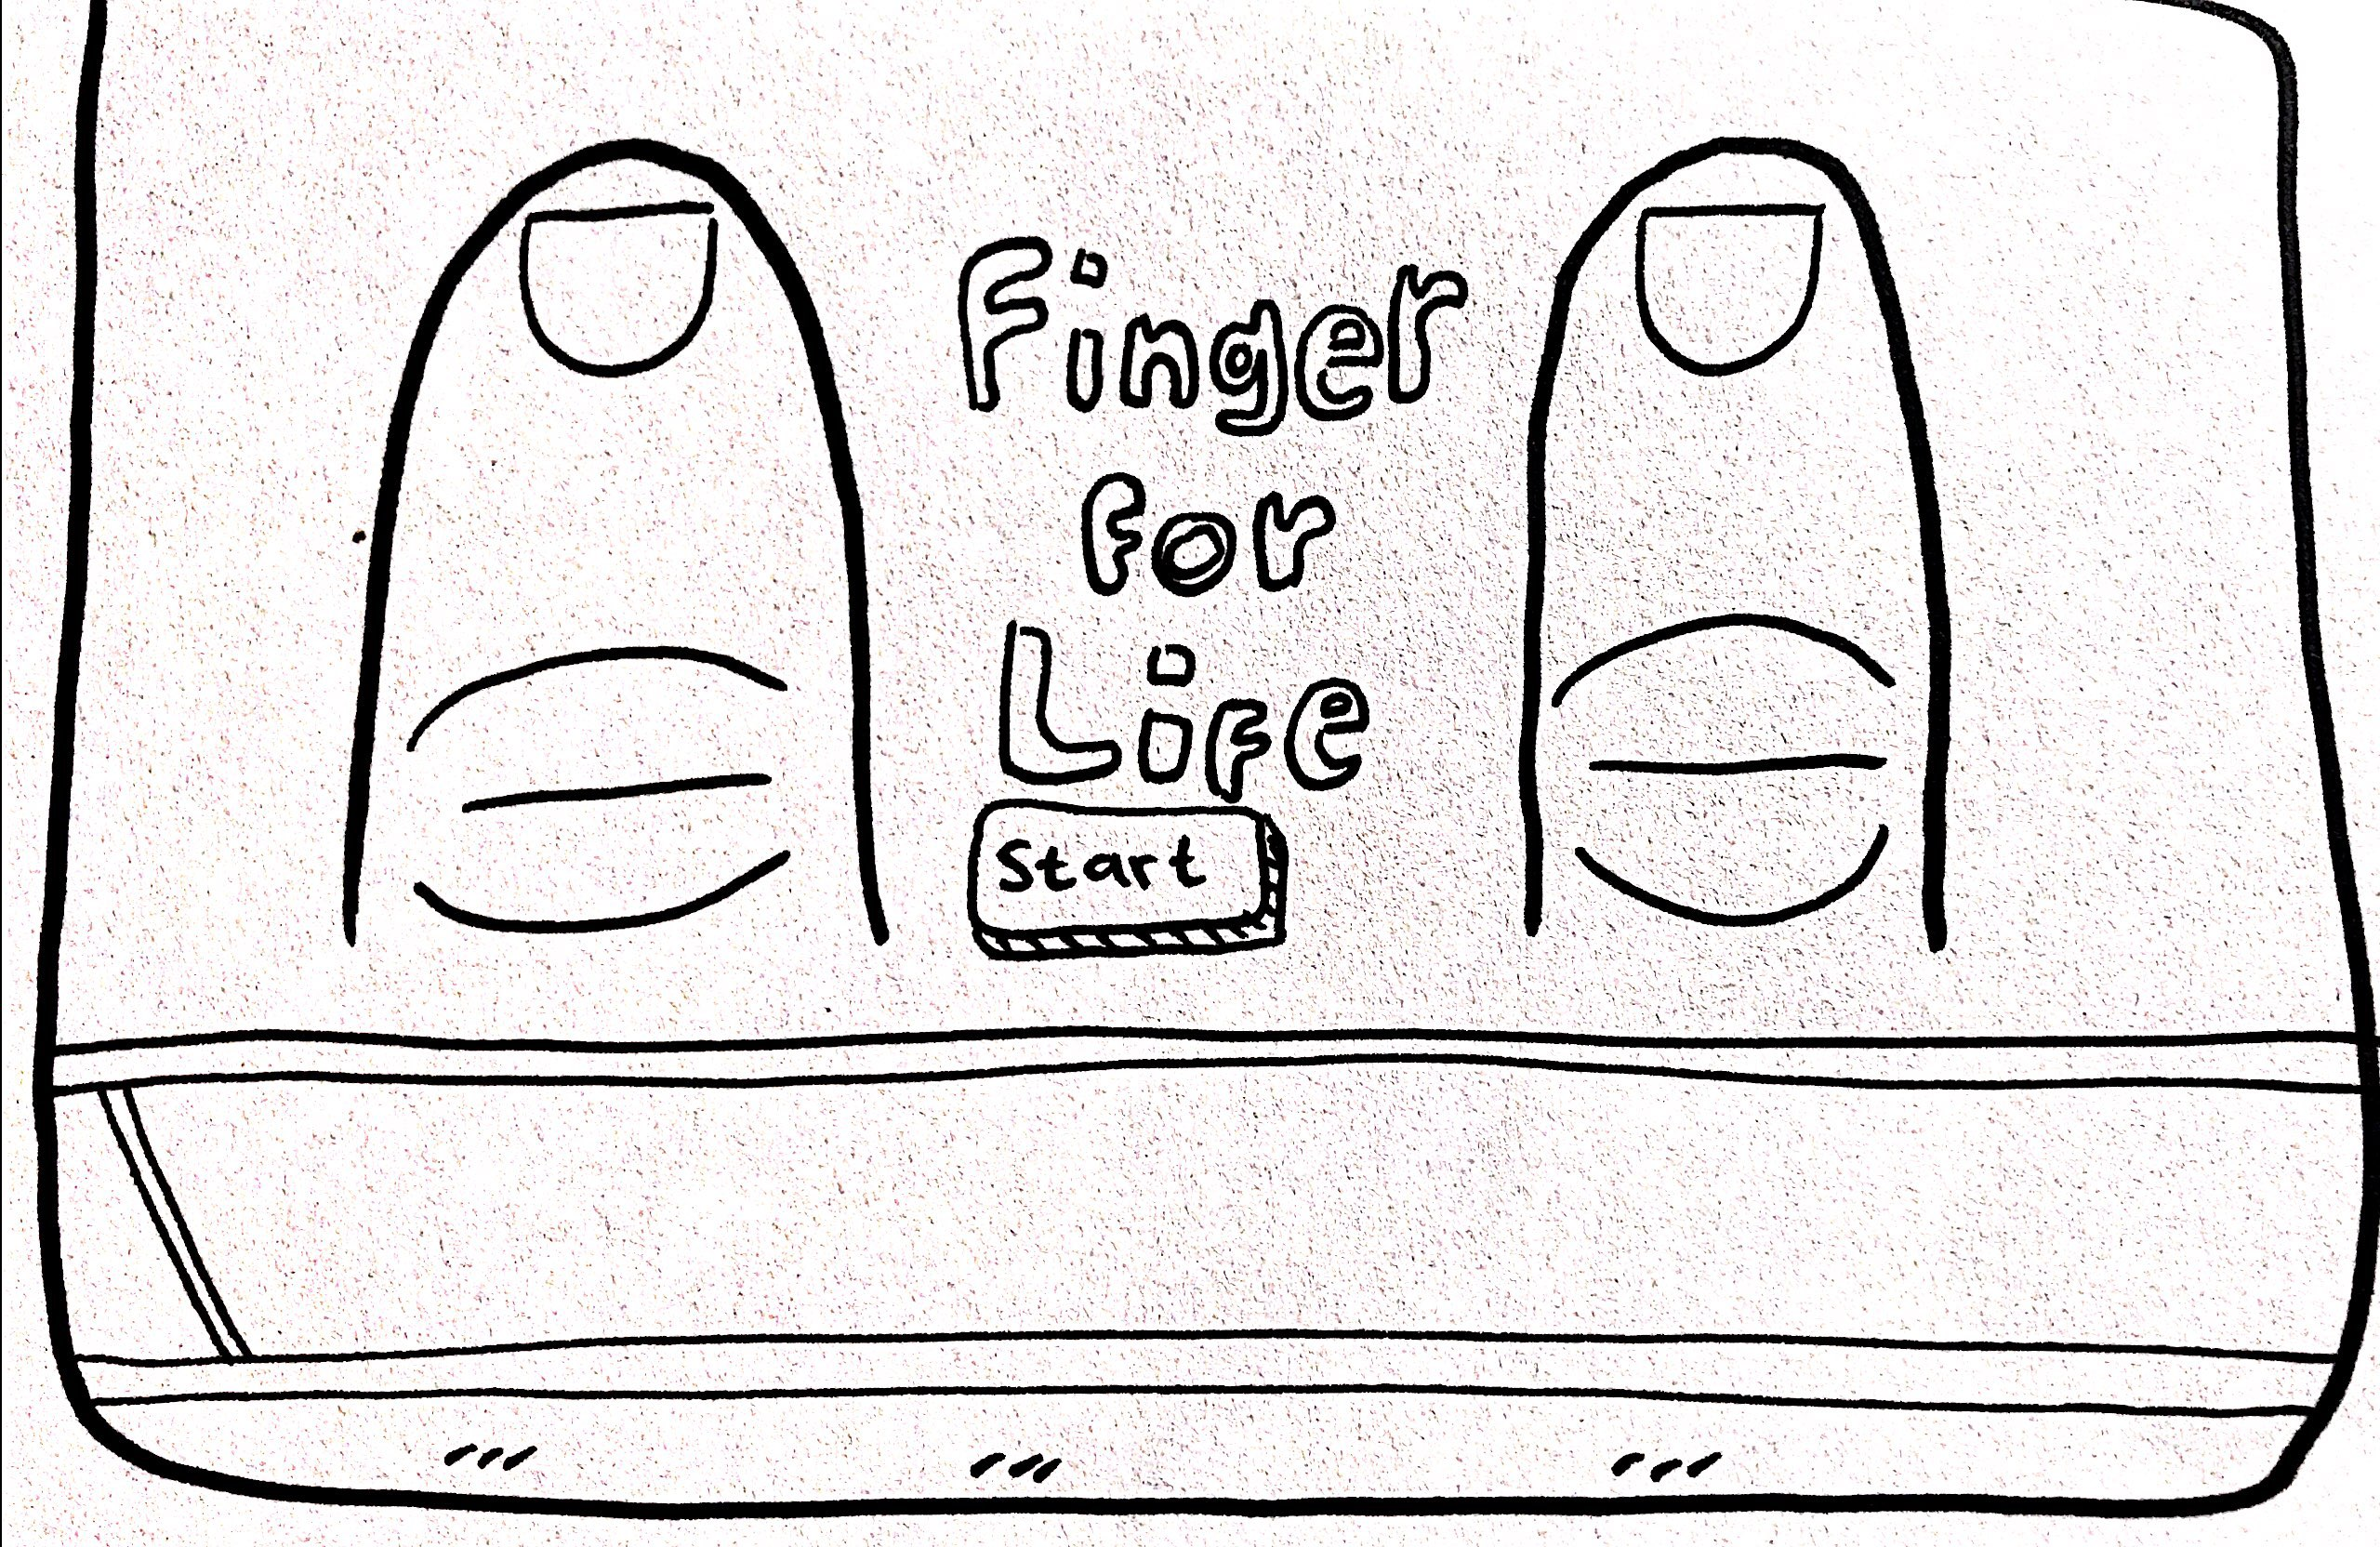
\includegraphics[scale=0.1]{Gambar/web1_home}
			\caption{Tampilan awal web}
			\label{fig:1_web1_home}
		\end{figure}
	
		\begin{figure}[H]
			\centering
			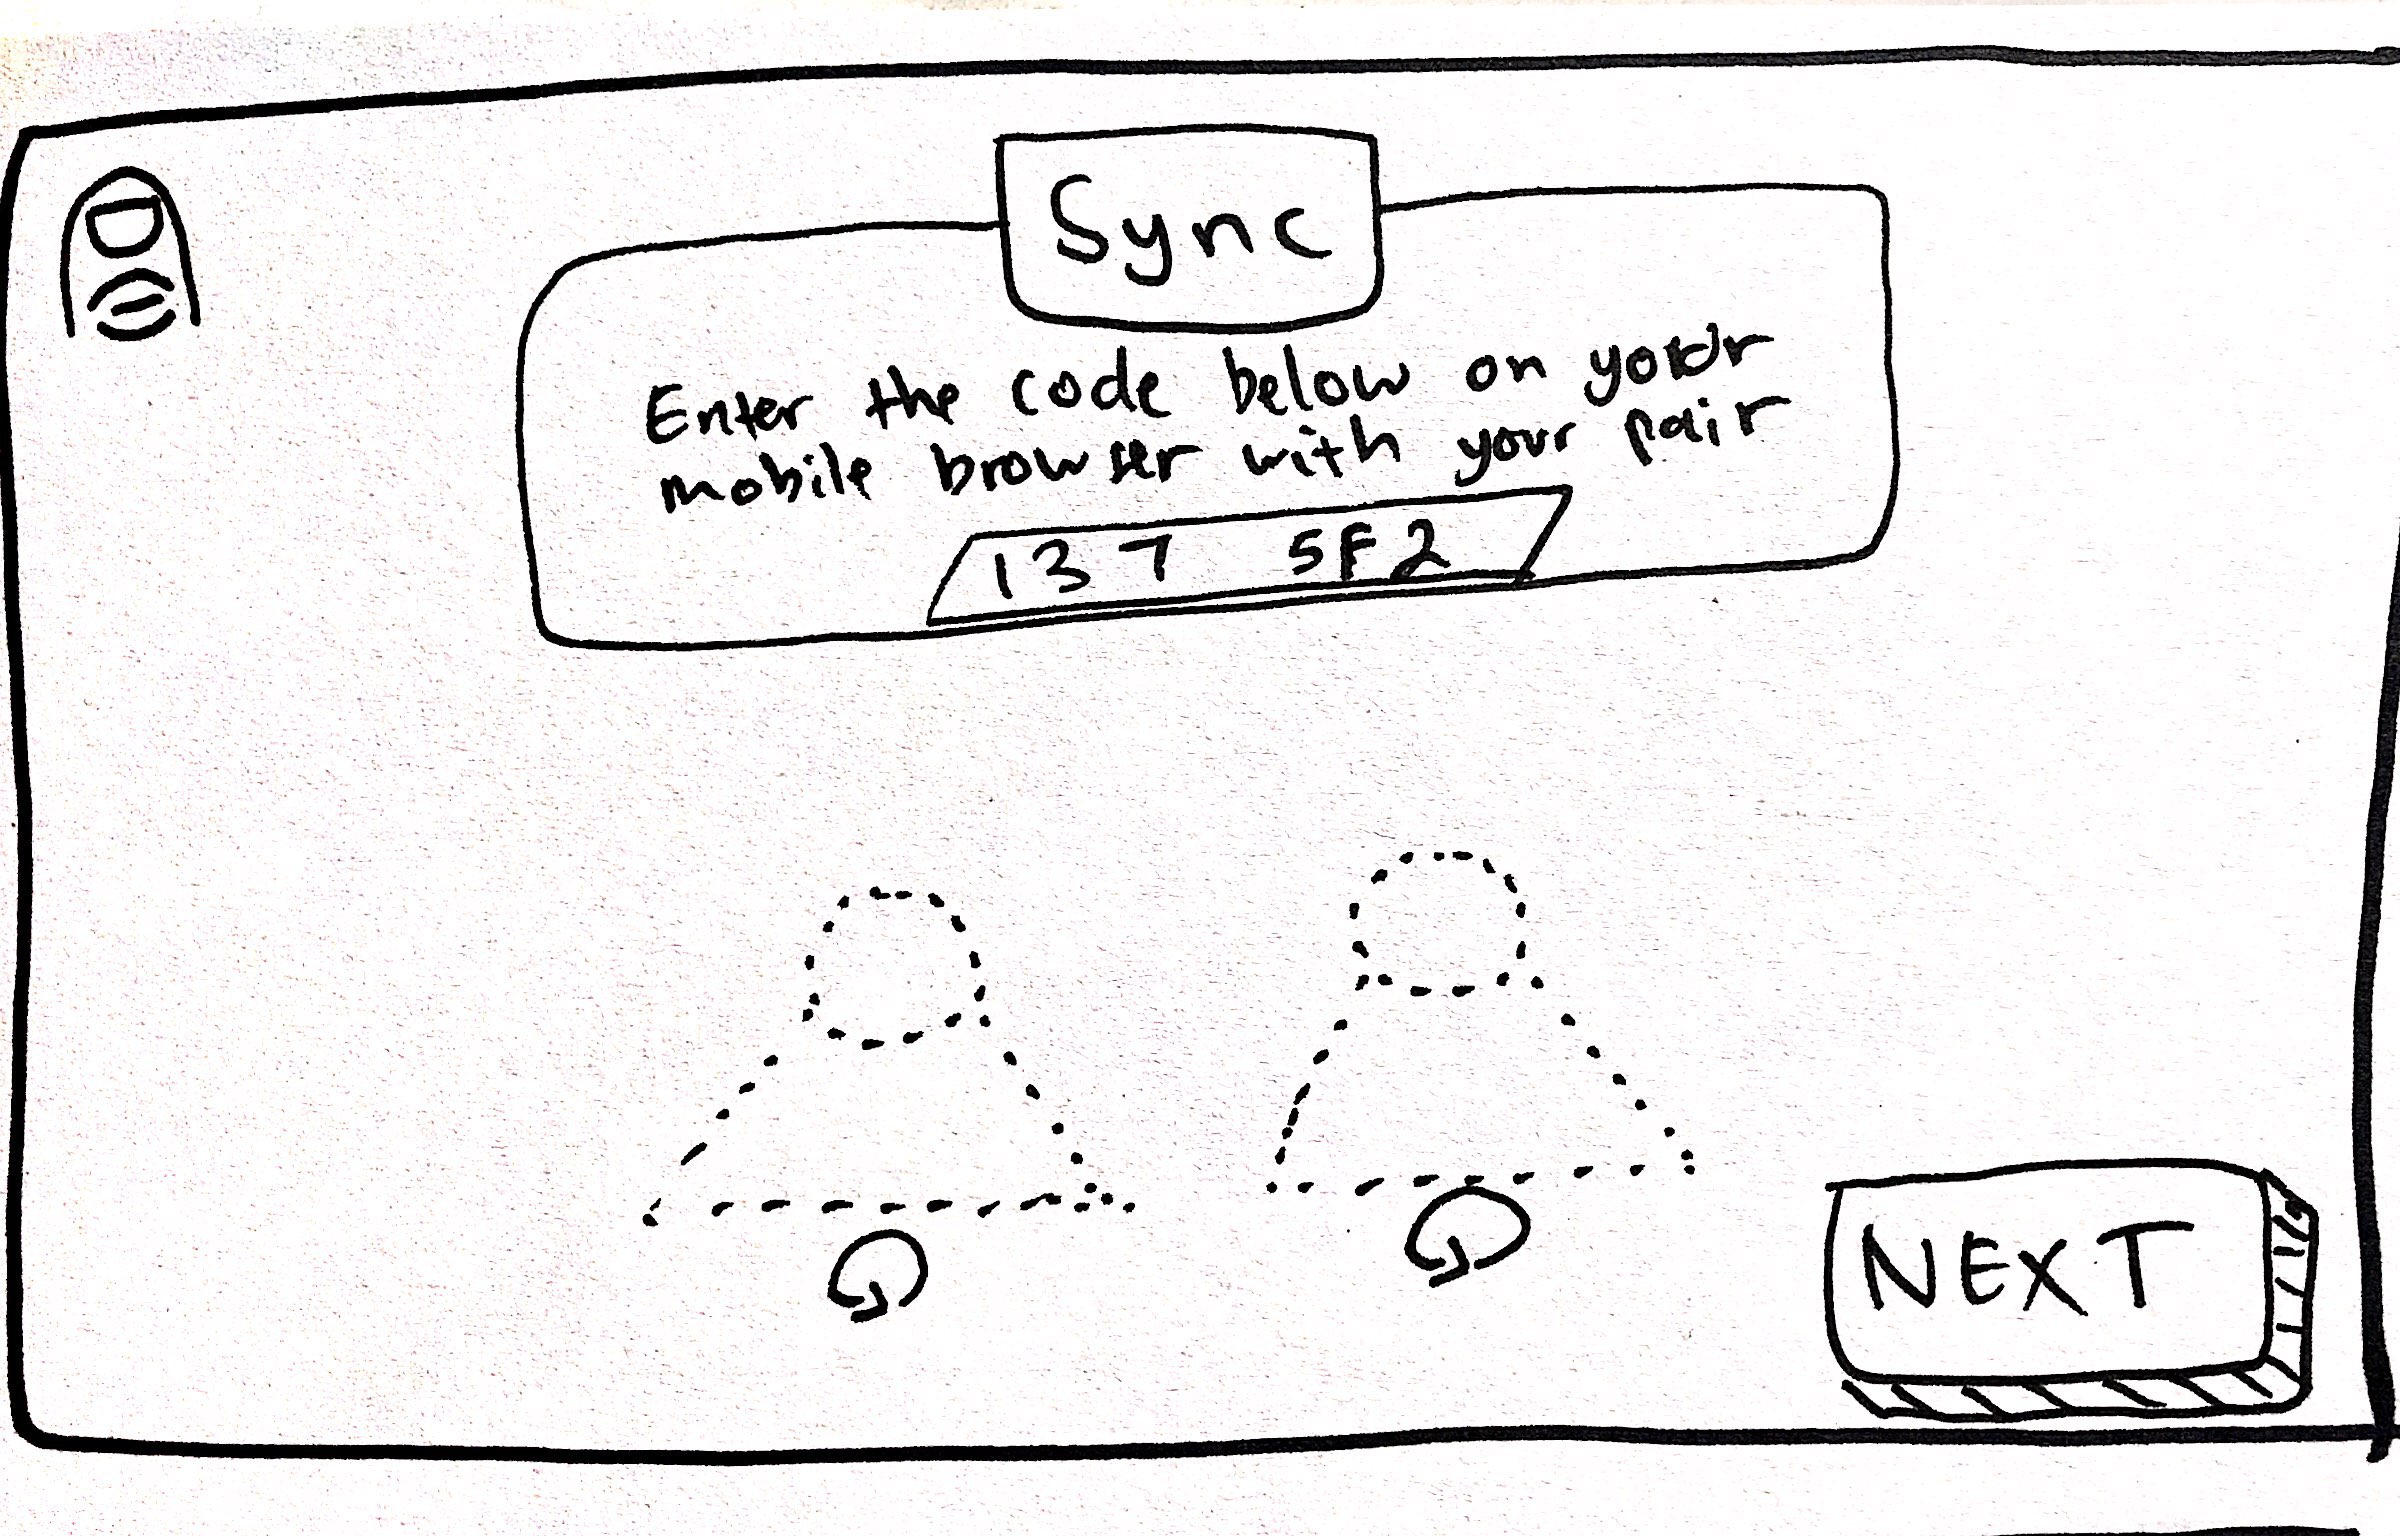
\includegraphics[scale=0.1]{Gambar/web2_sync1}
			\caption{Para pemain yang akan melakukan proses \textit{sync}}
			\label{fig:2_web2_sync1}
		\end{figure}
	
		\begin{figure}[H]
			\centering
			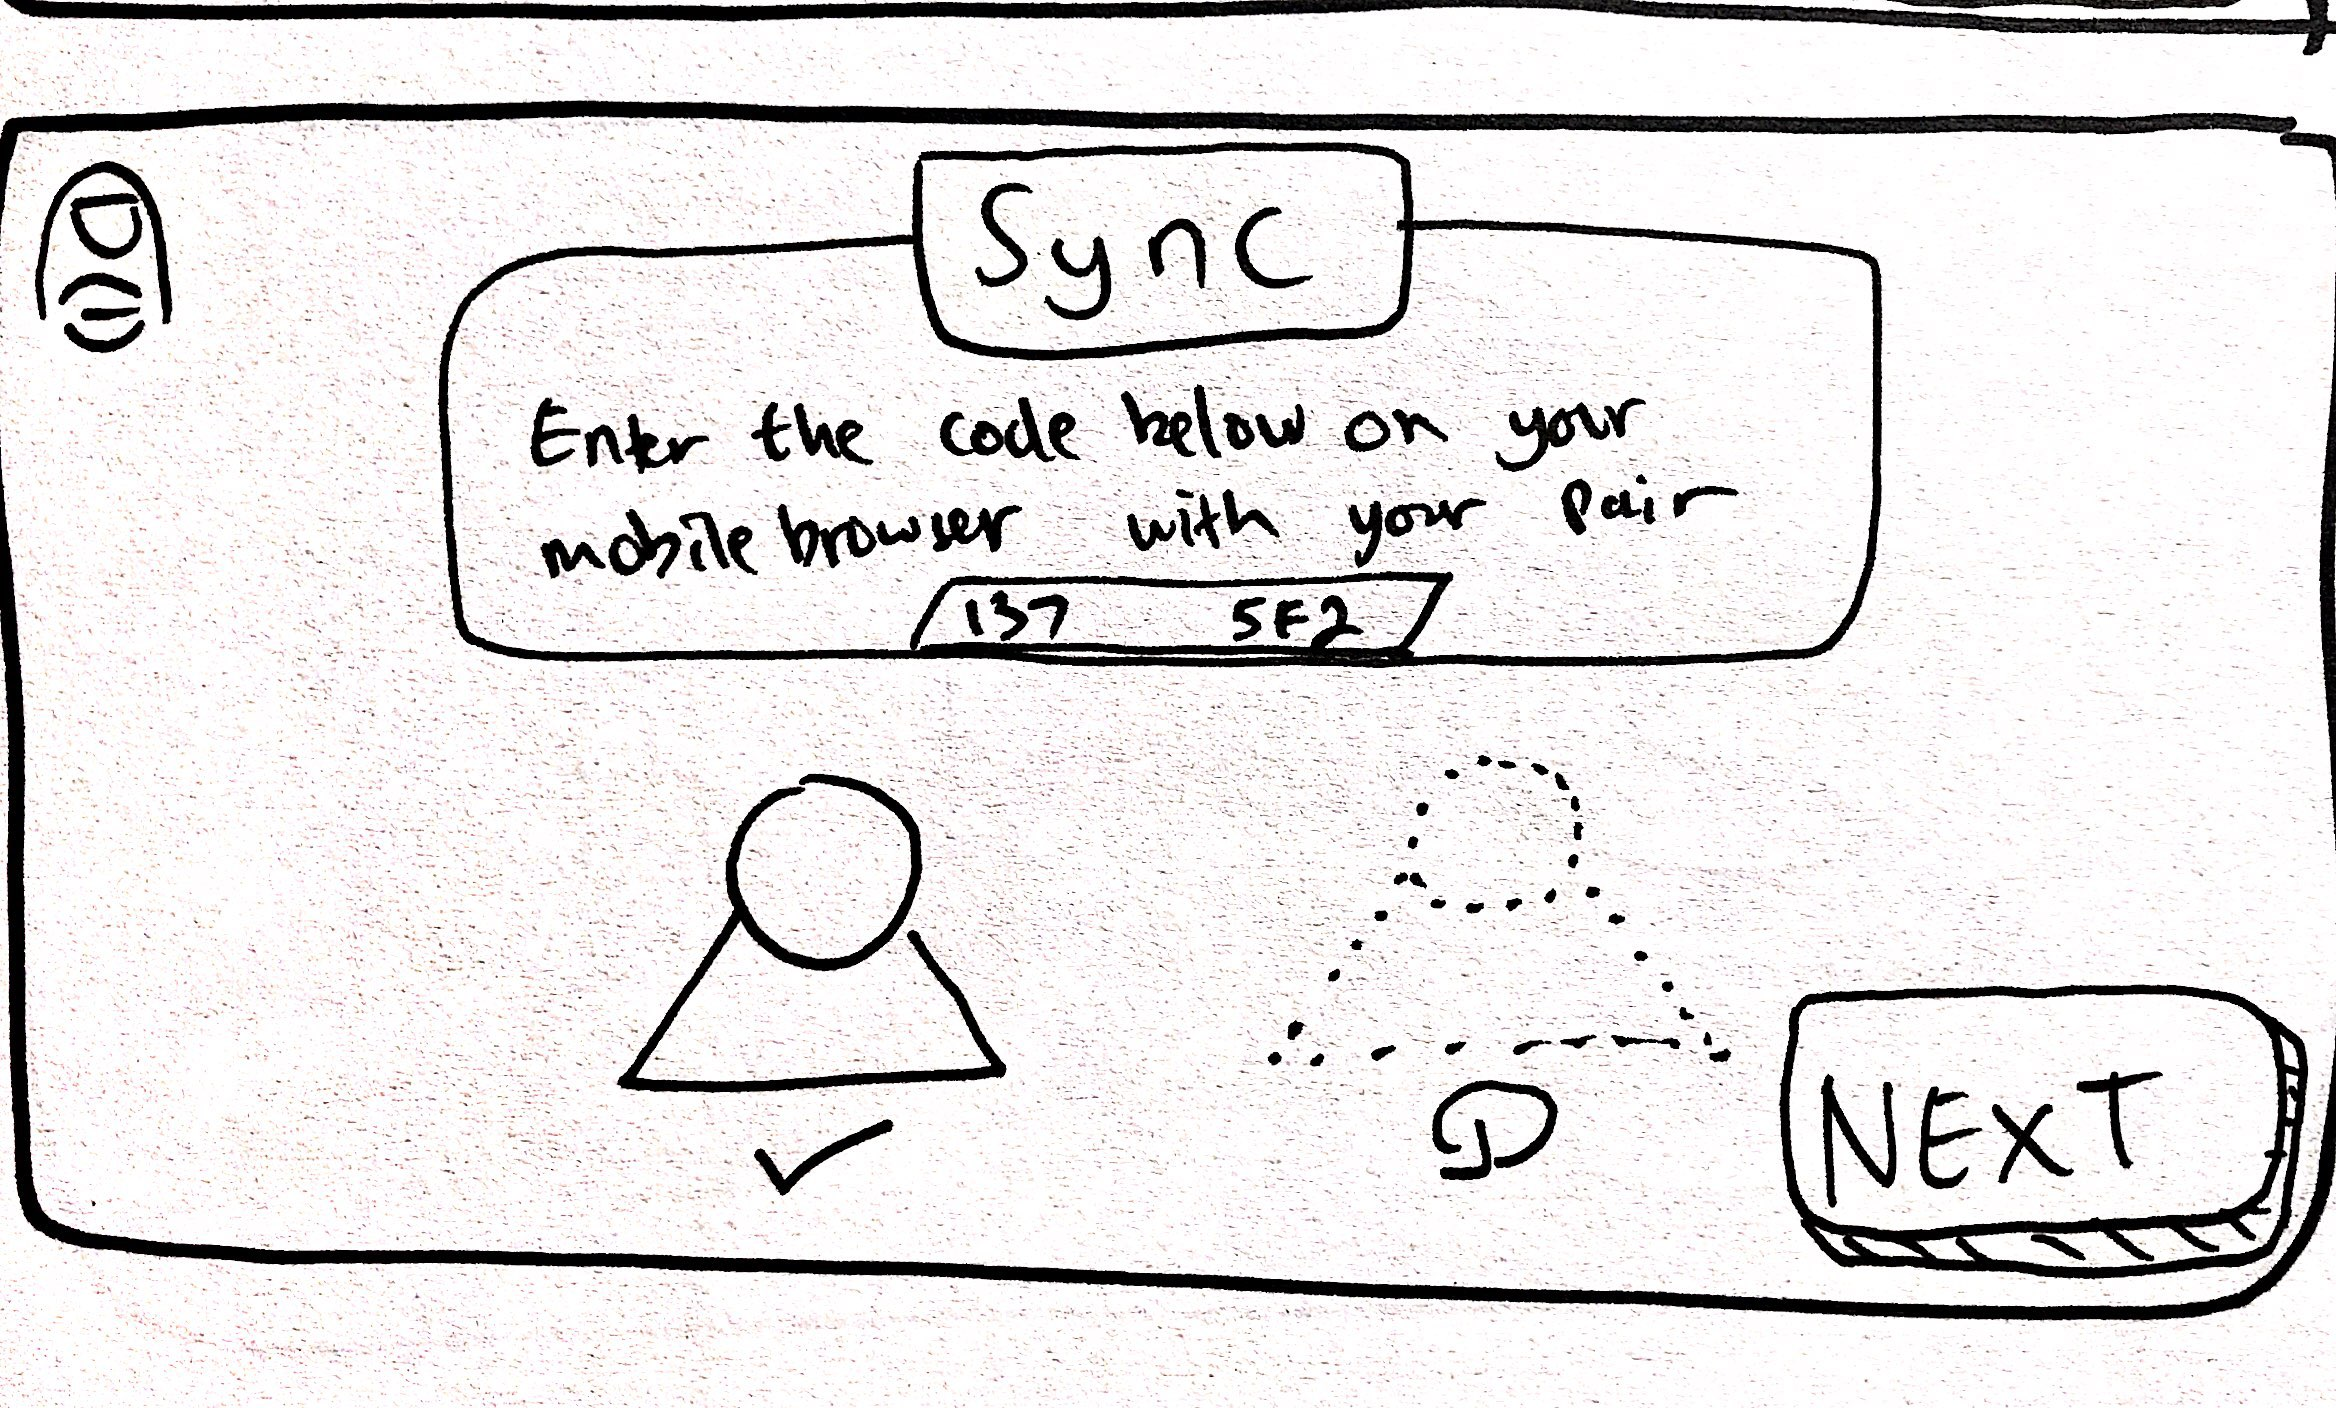
\includegraphics[scale=0.1]{Gambar/web3_sync2}
			\caption{Pemain pertama yang sudah melakukan proses \textit{sync}}
			\label{fig:3_web3_sync2}
		\end{figure}
	
		\begin{figure}[H]
			\centering
			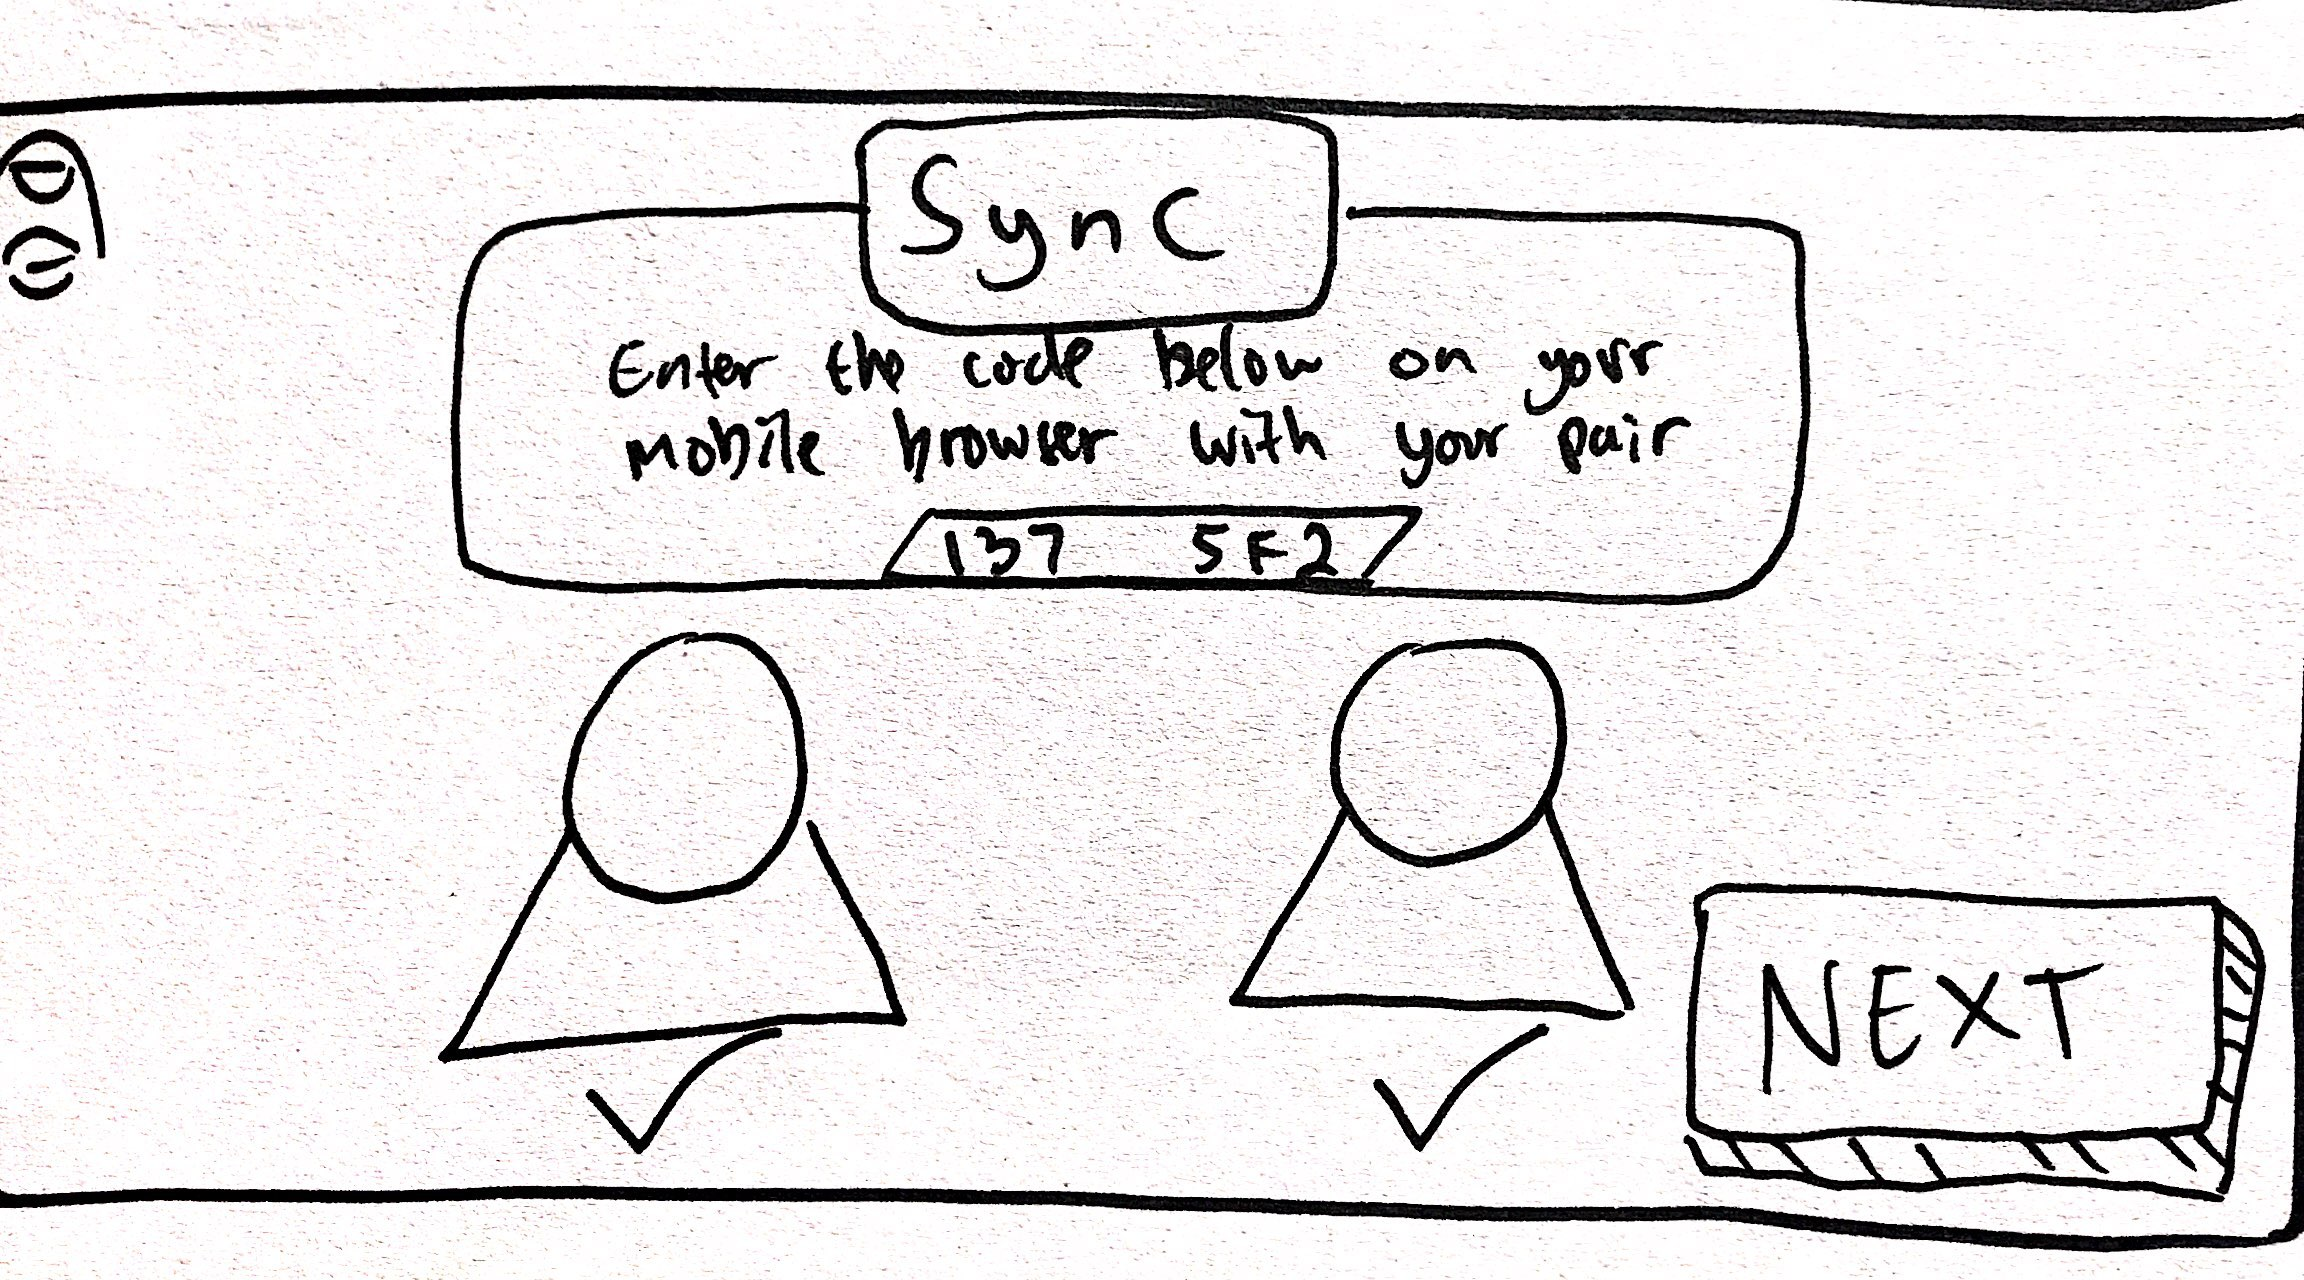
\includegraphics[scale=0.1]{Gambar/web4_sync3}
			\caption{Pemain kedua yang sudah melakukan proses \textit{sync}}
			\label{fig:4_web4_sync3}
		\end{figure}
	
		\begin{figure}[H]
			\centering
			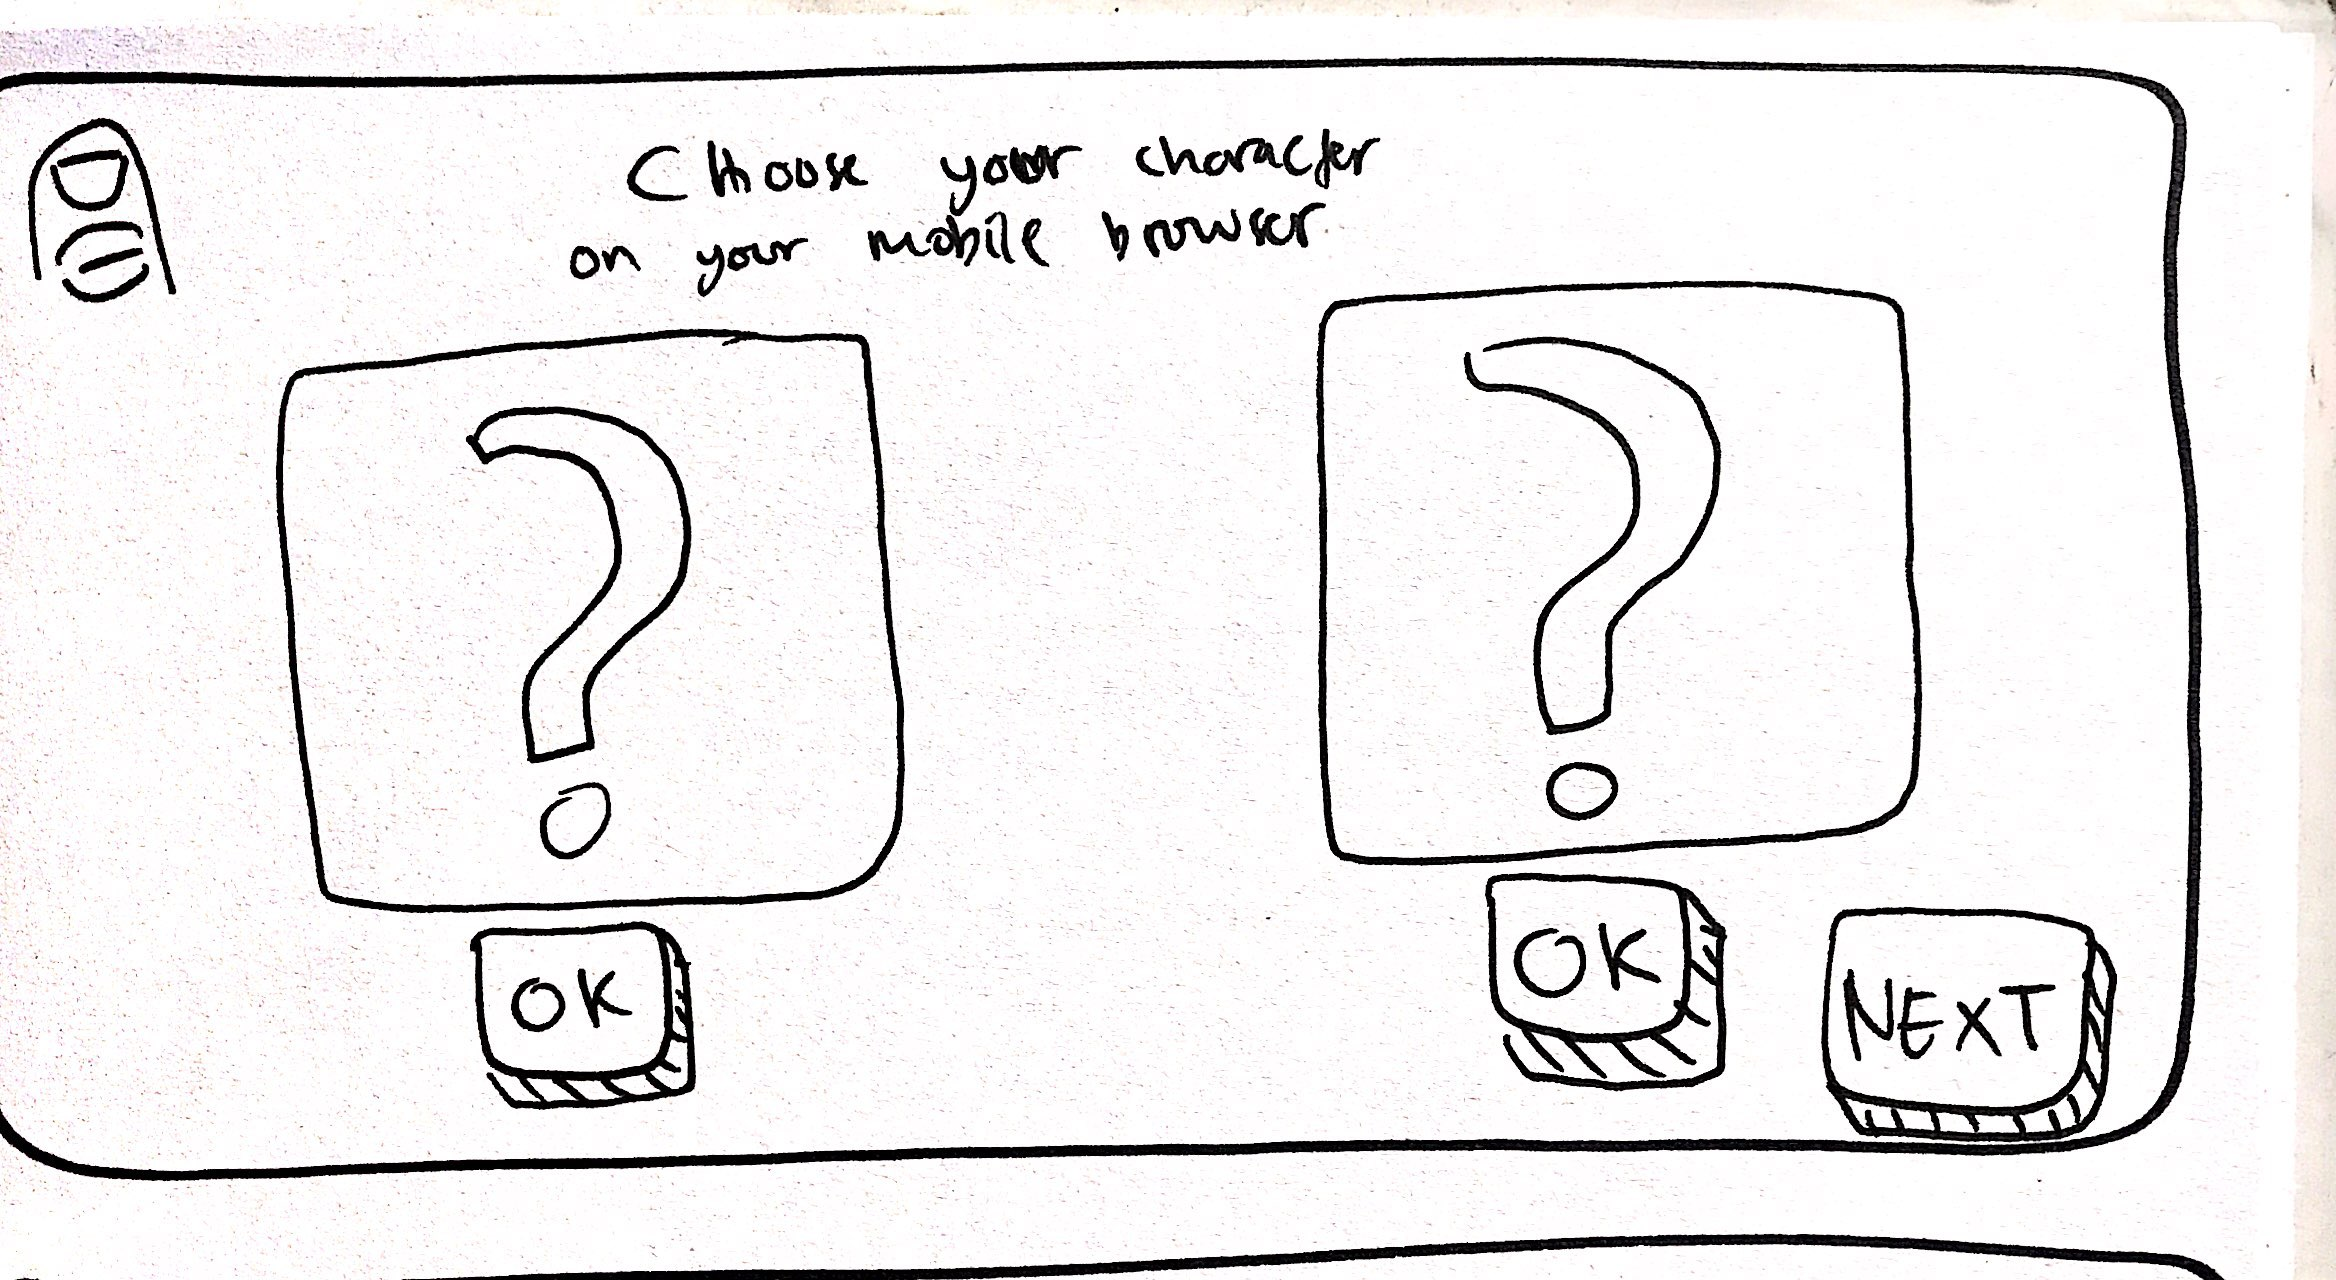
\includegraphics[scale=0.1]{Gambar/web5_char1}
			\caption{Para pemain yang akan memilih karakter}
			\label{fig:5_web5_char1}
		\end{figure}
	
		\begin{figure}[H]
			\centering
			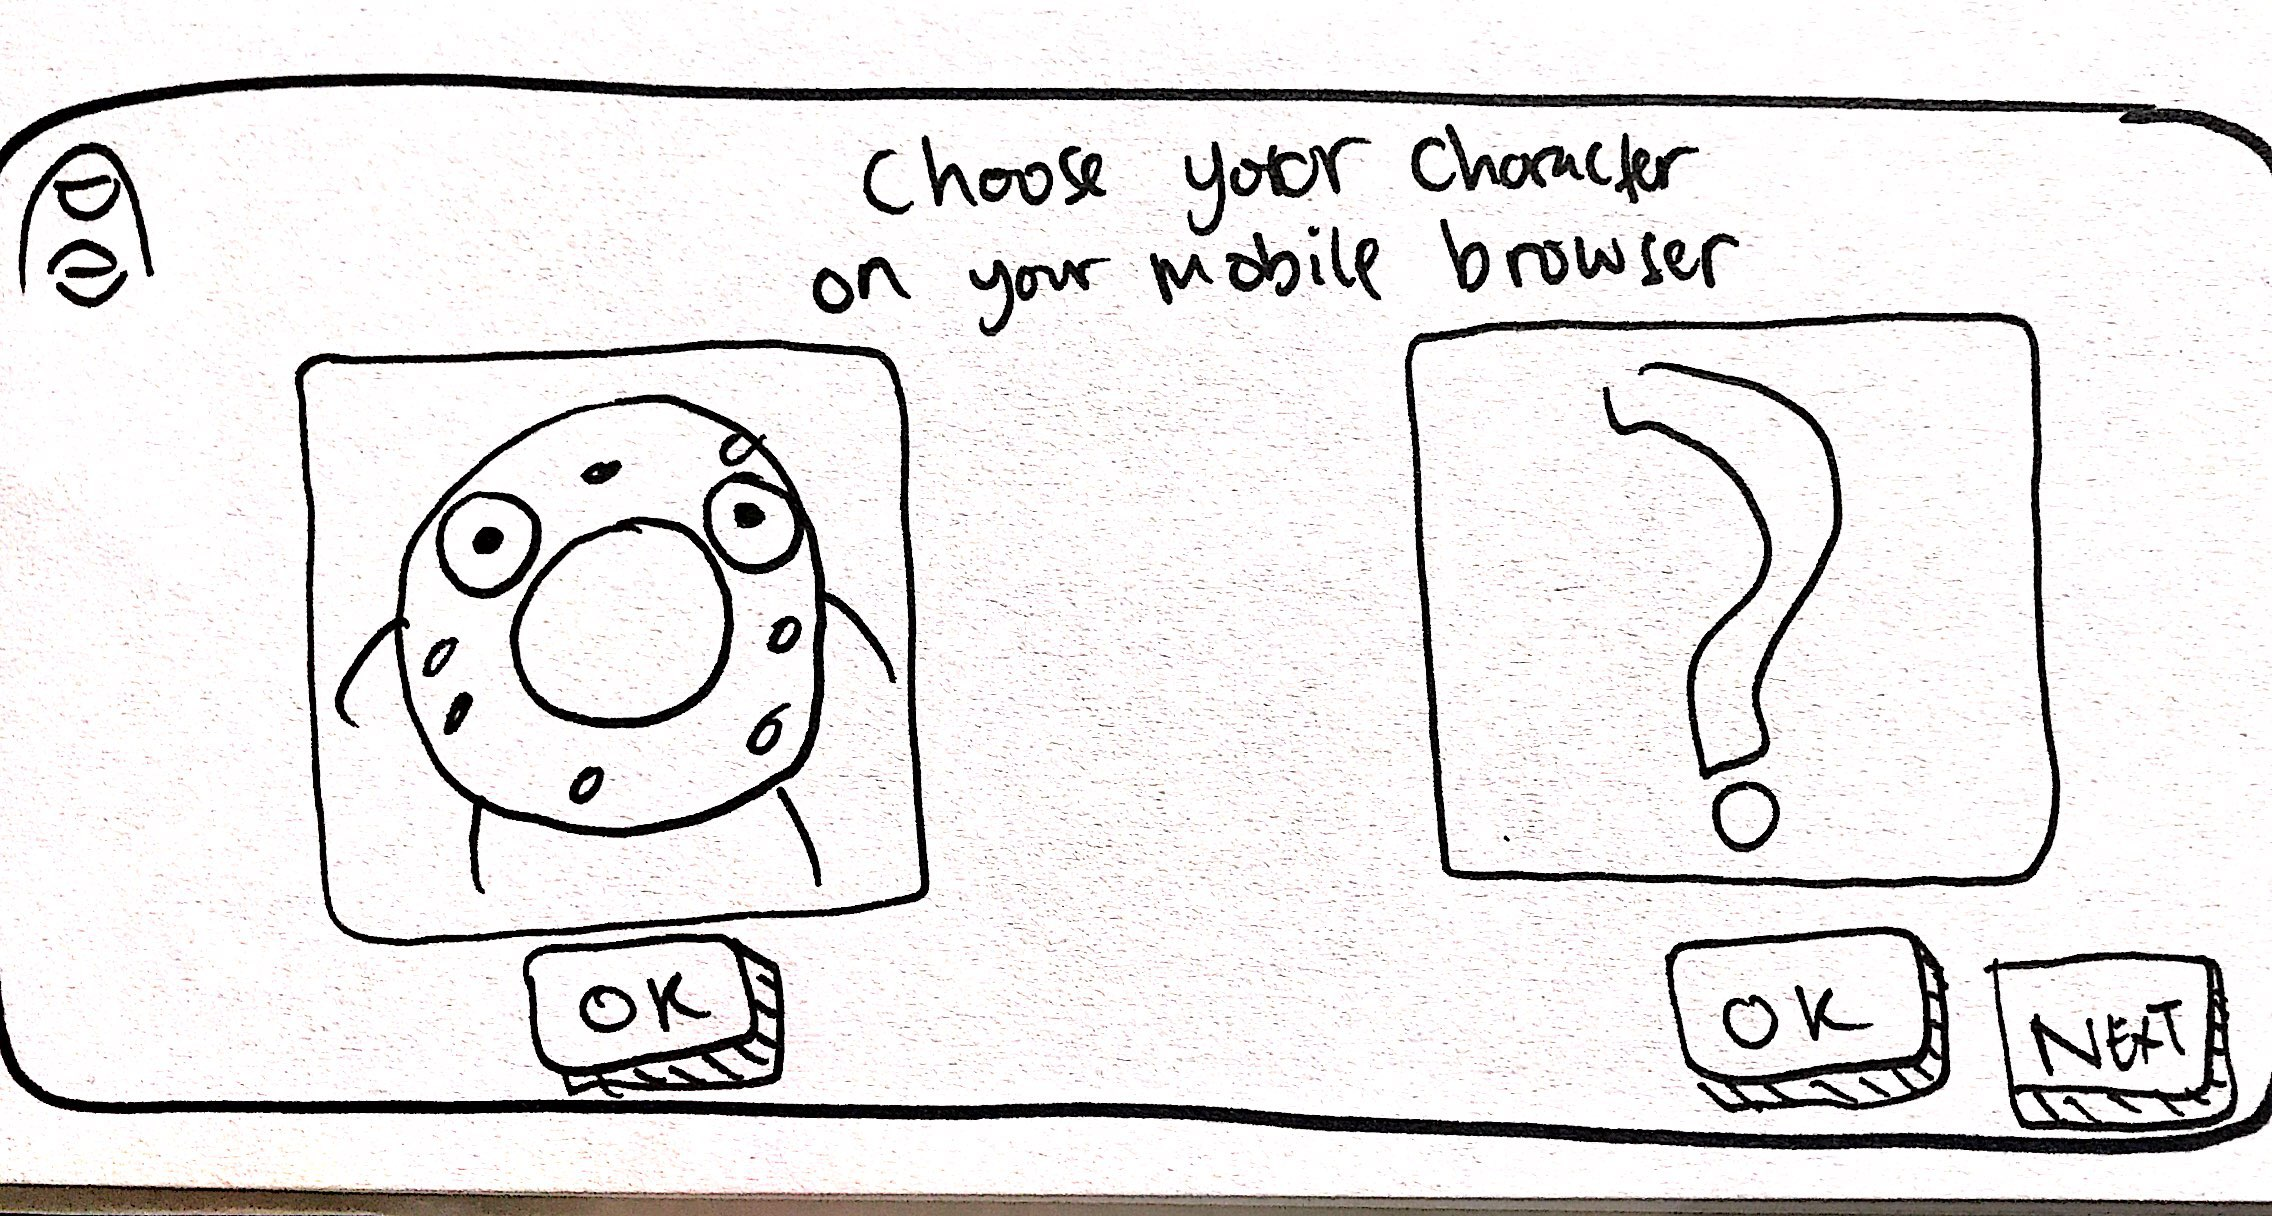
\includegraphics[scale=0.1]{Gambar/web6_char2}
			\caption{Pemain pertama yang sudah memilih karakter.}
			\label{fig:6_web6_char2}
		\end{figure}
	
		\begin{figure}[H]
			\centering
			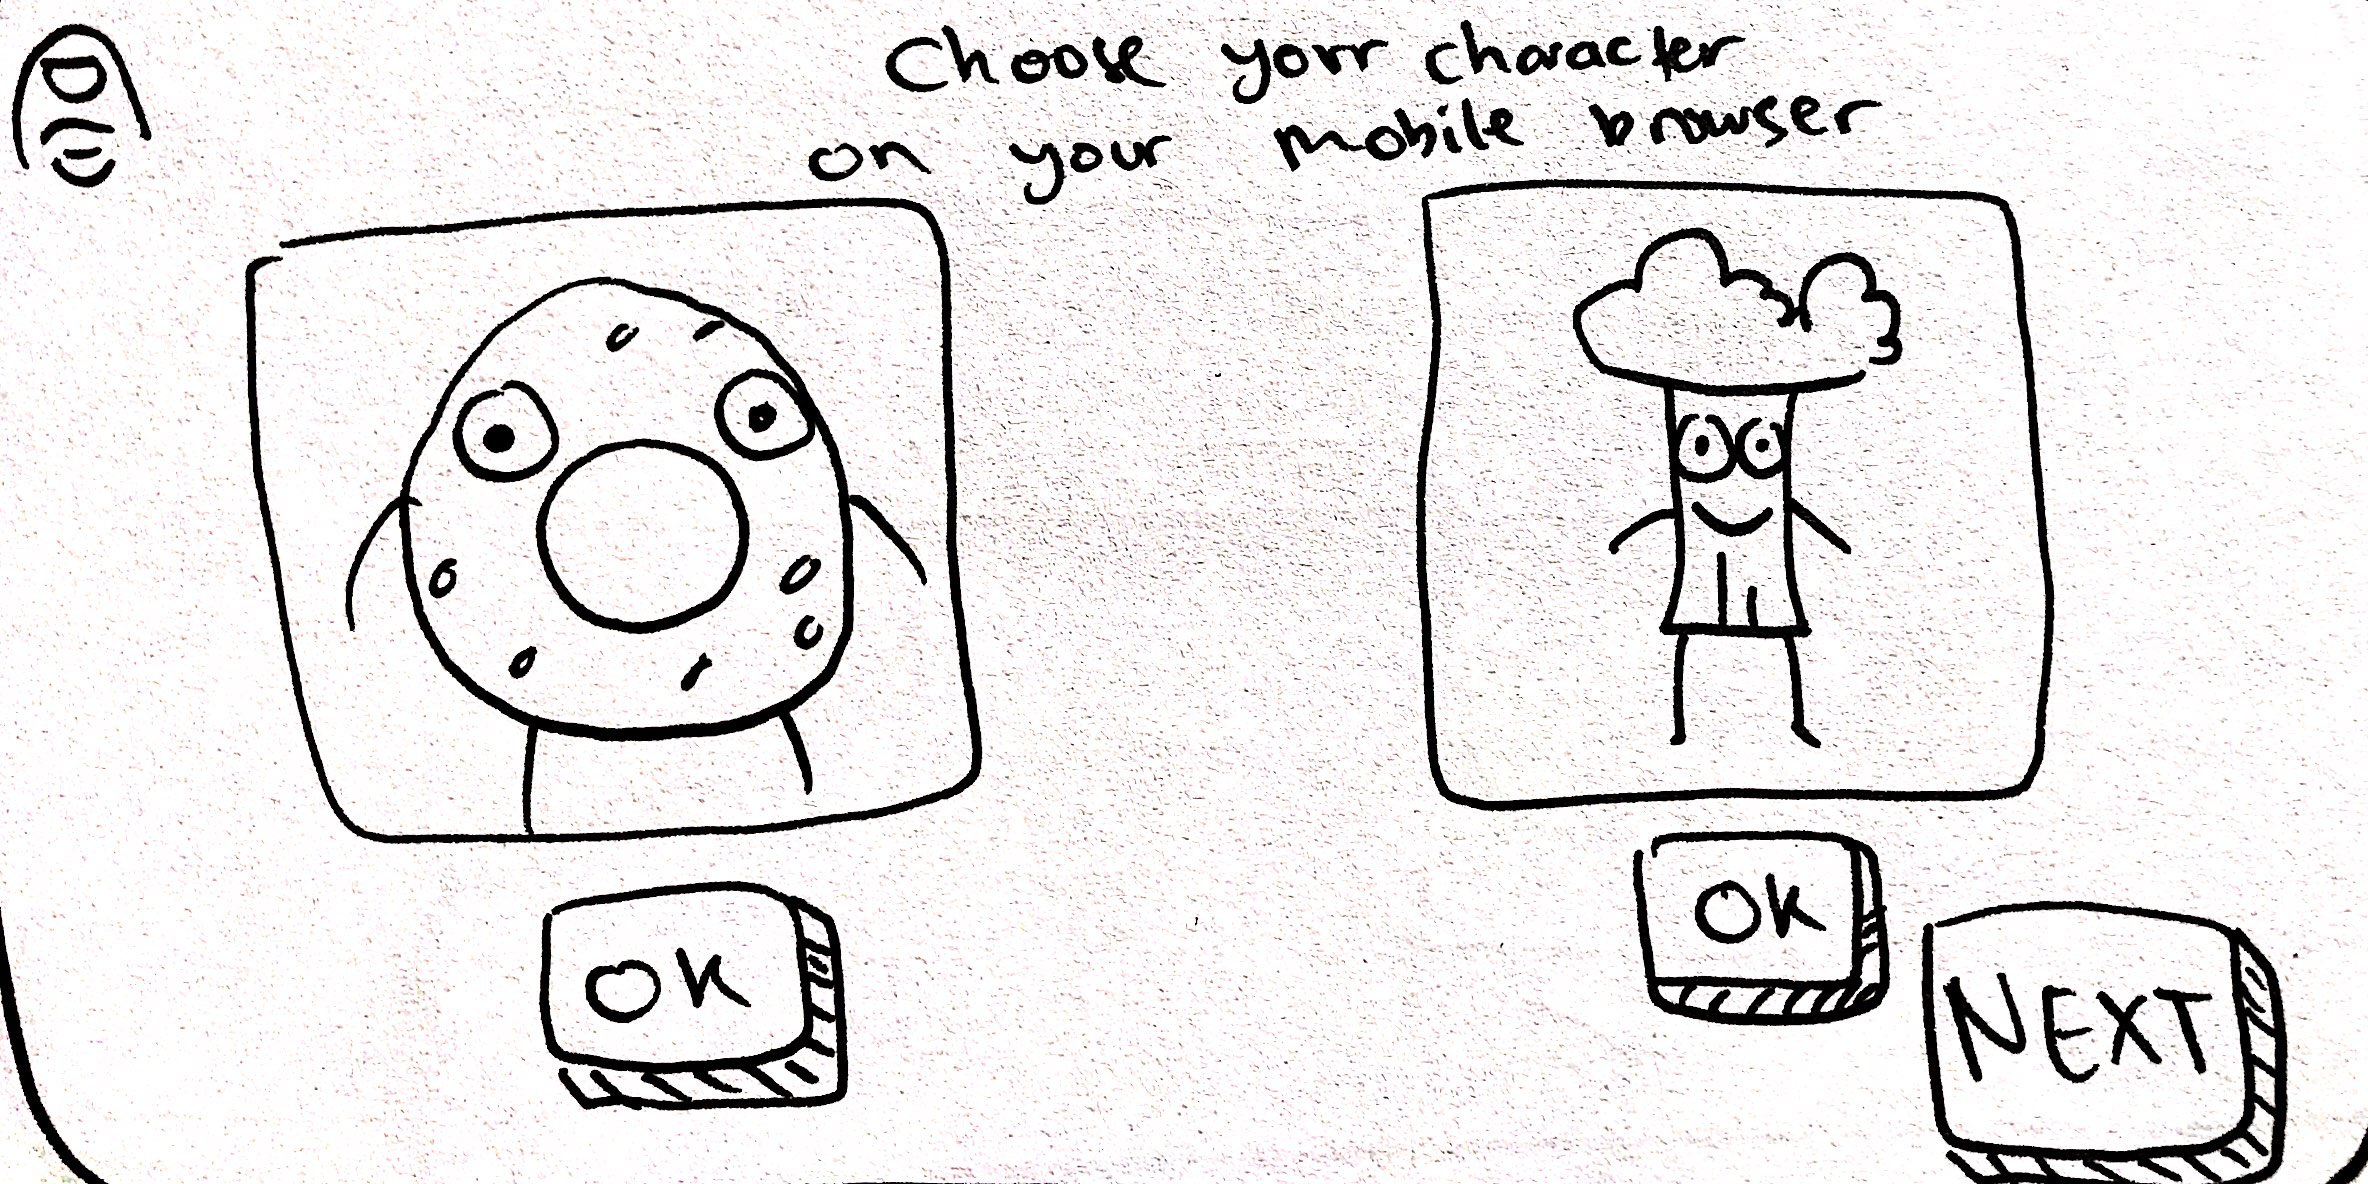
\includegraphics[scale=0.1]{Gambar/web7_char3}
			\caption{Pemain kedua yang sudah memilih karakter.}
			\label{fig:7_web7_char3}
		\end{figure}
	
		\begin{figure}[H]
			\centering
			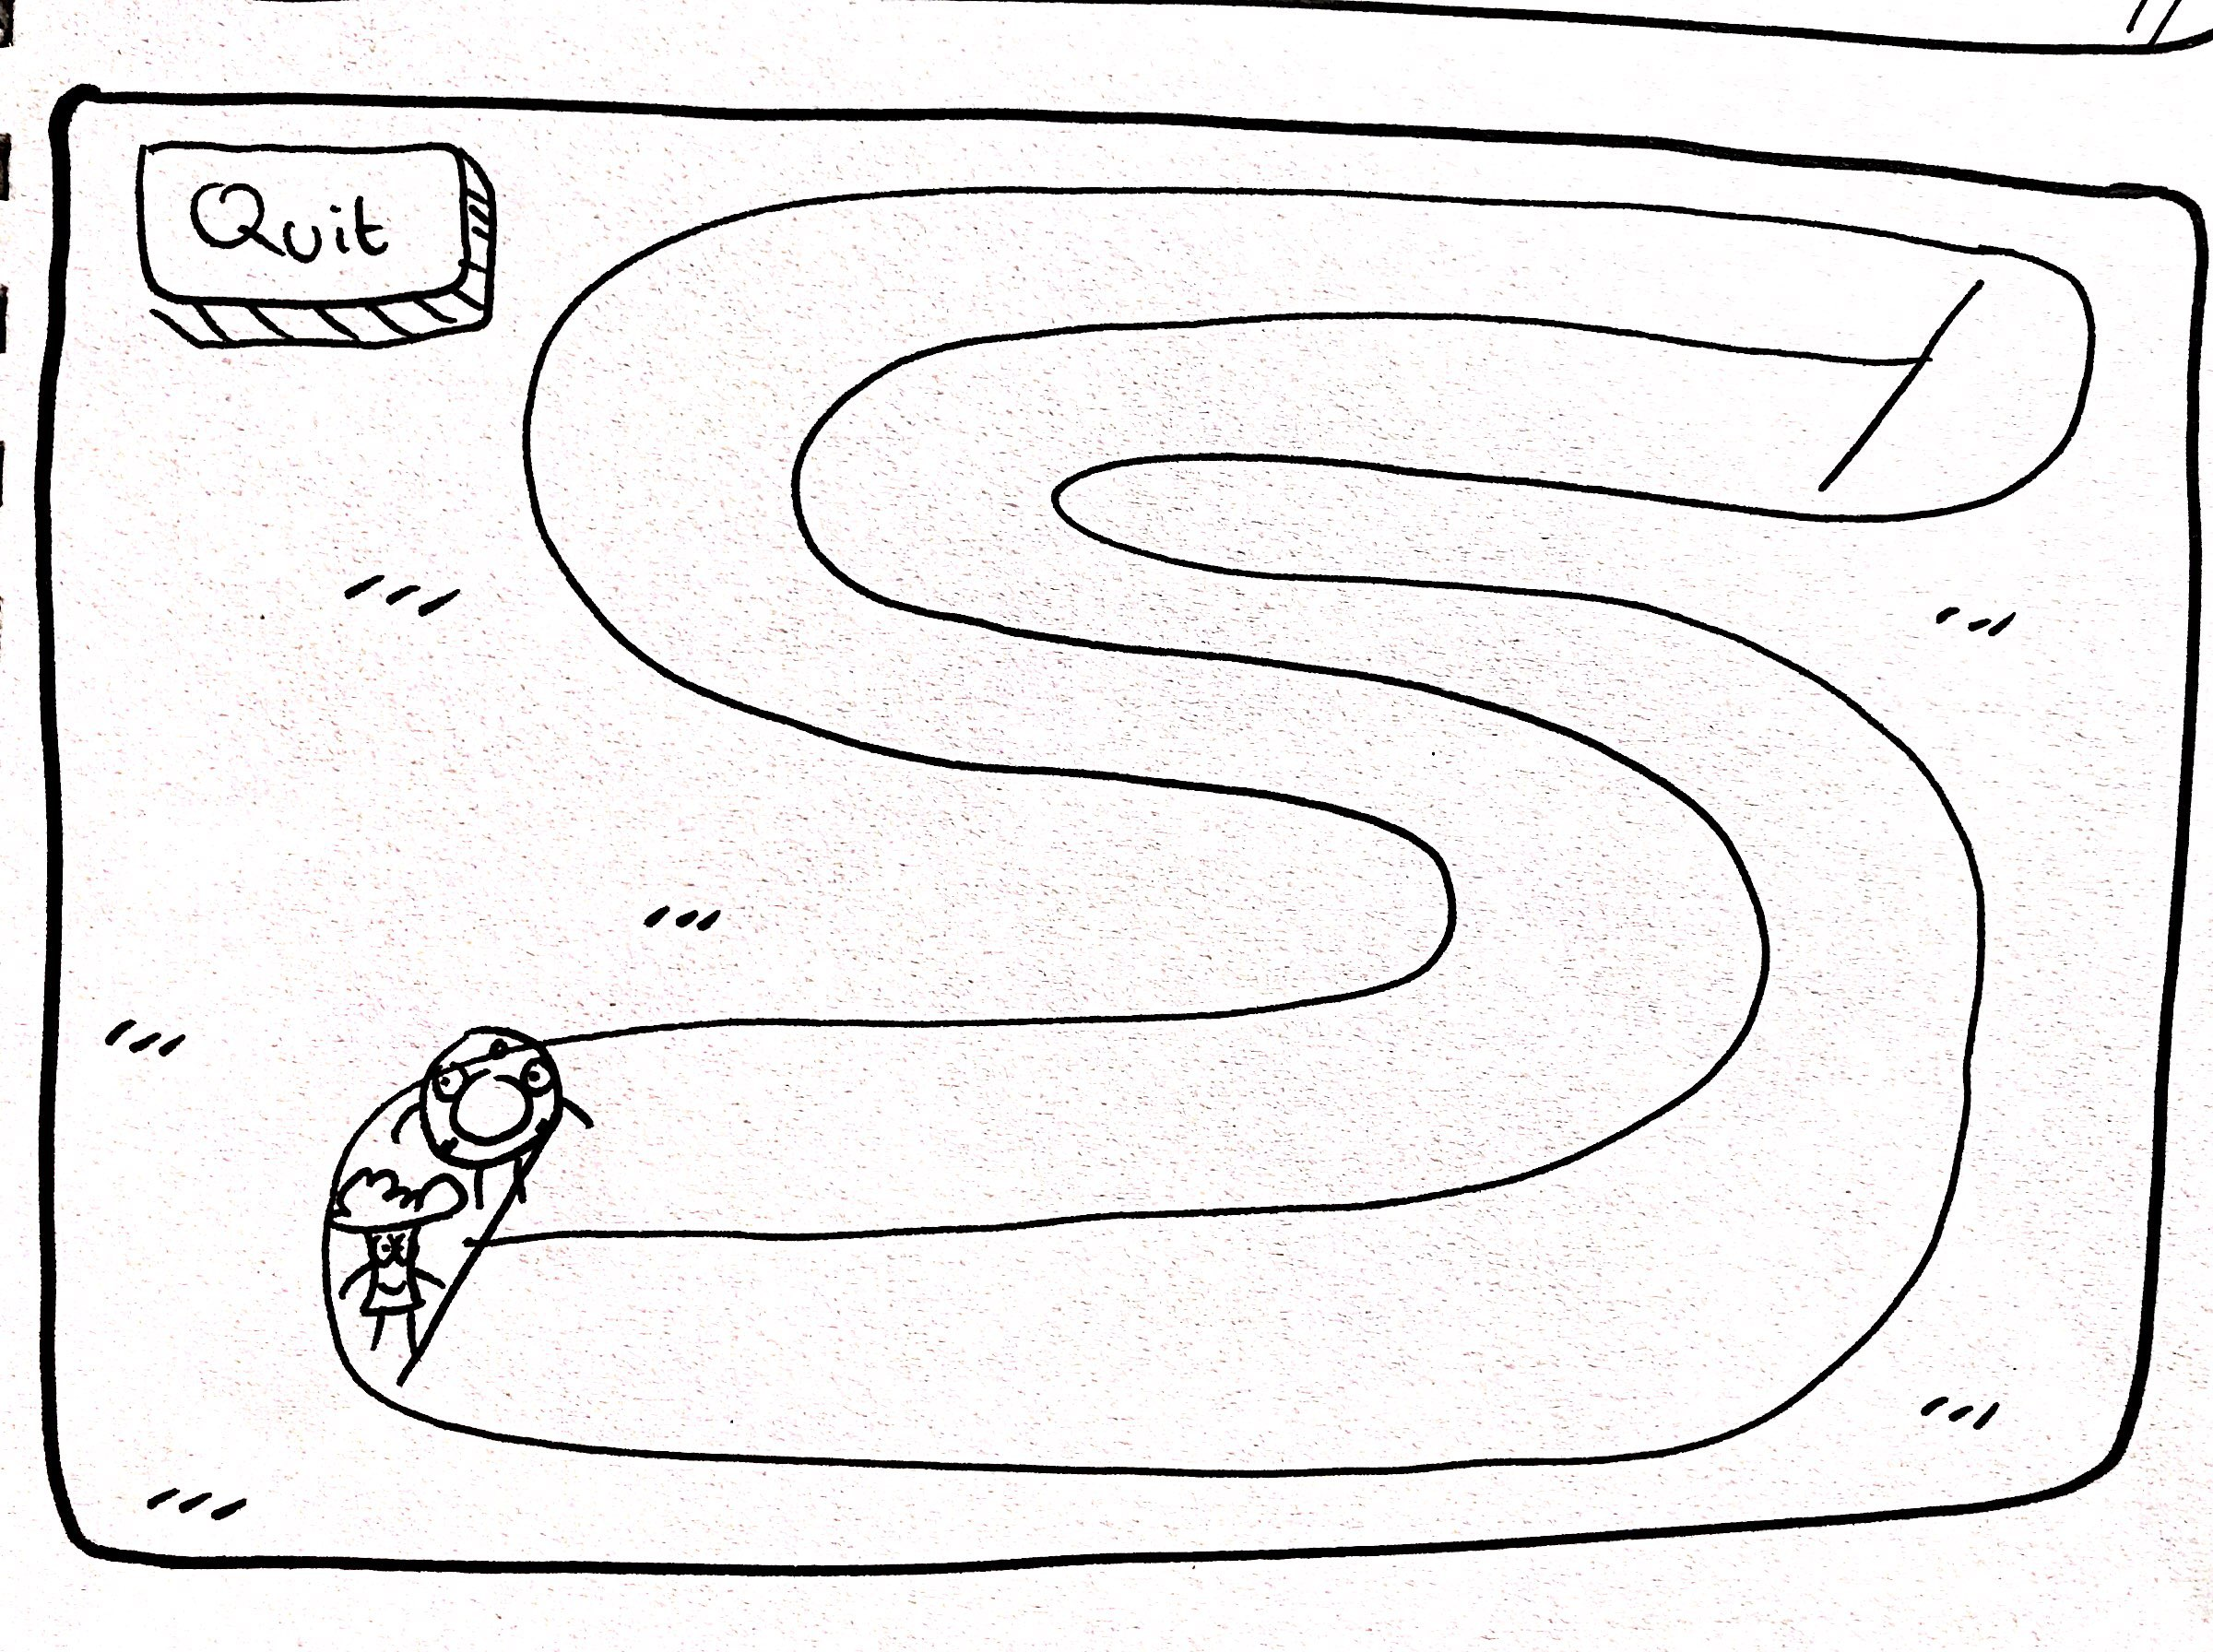
\includegraphics[scale=0.1]{Gambar/web8_run1}
			\caption{Kedua pemain yang akan siap memainkan permainan.}
			\label{fig:8_web8_run1}
		\end{figure}
	
		\begin{figure}[H]
			\centering
			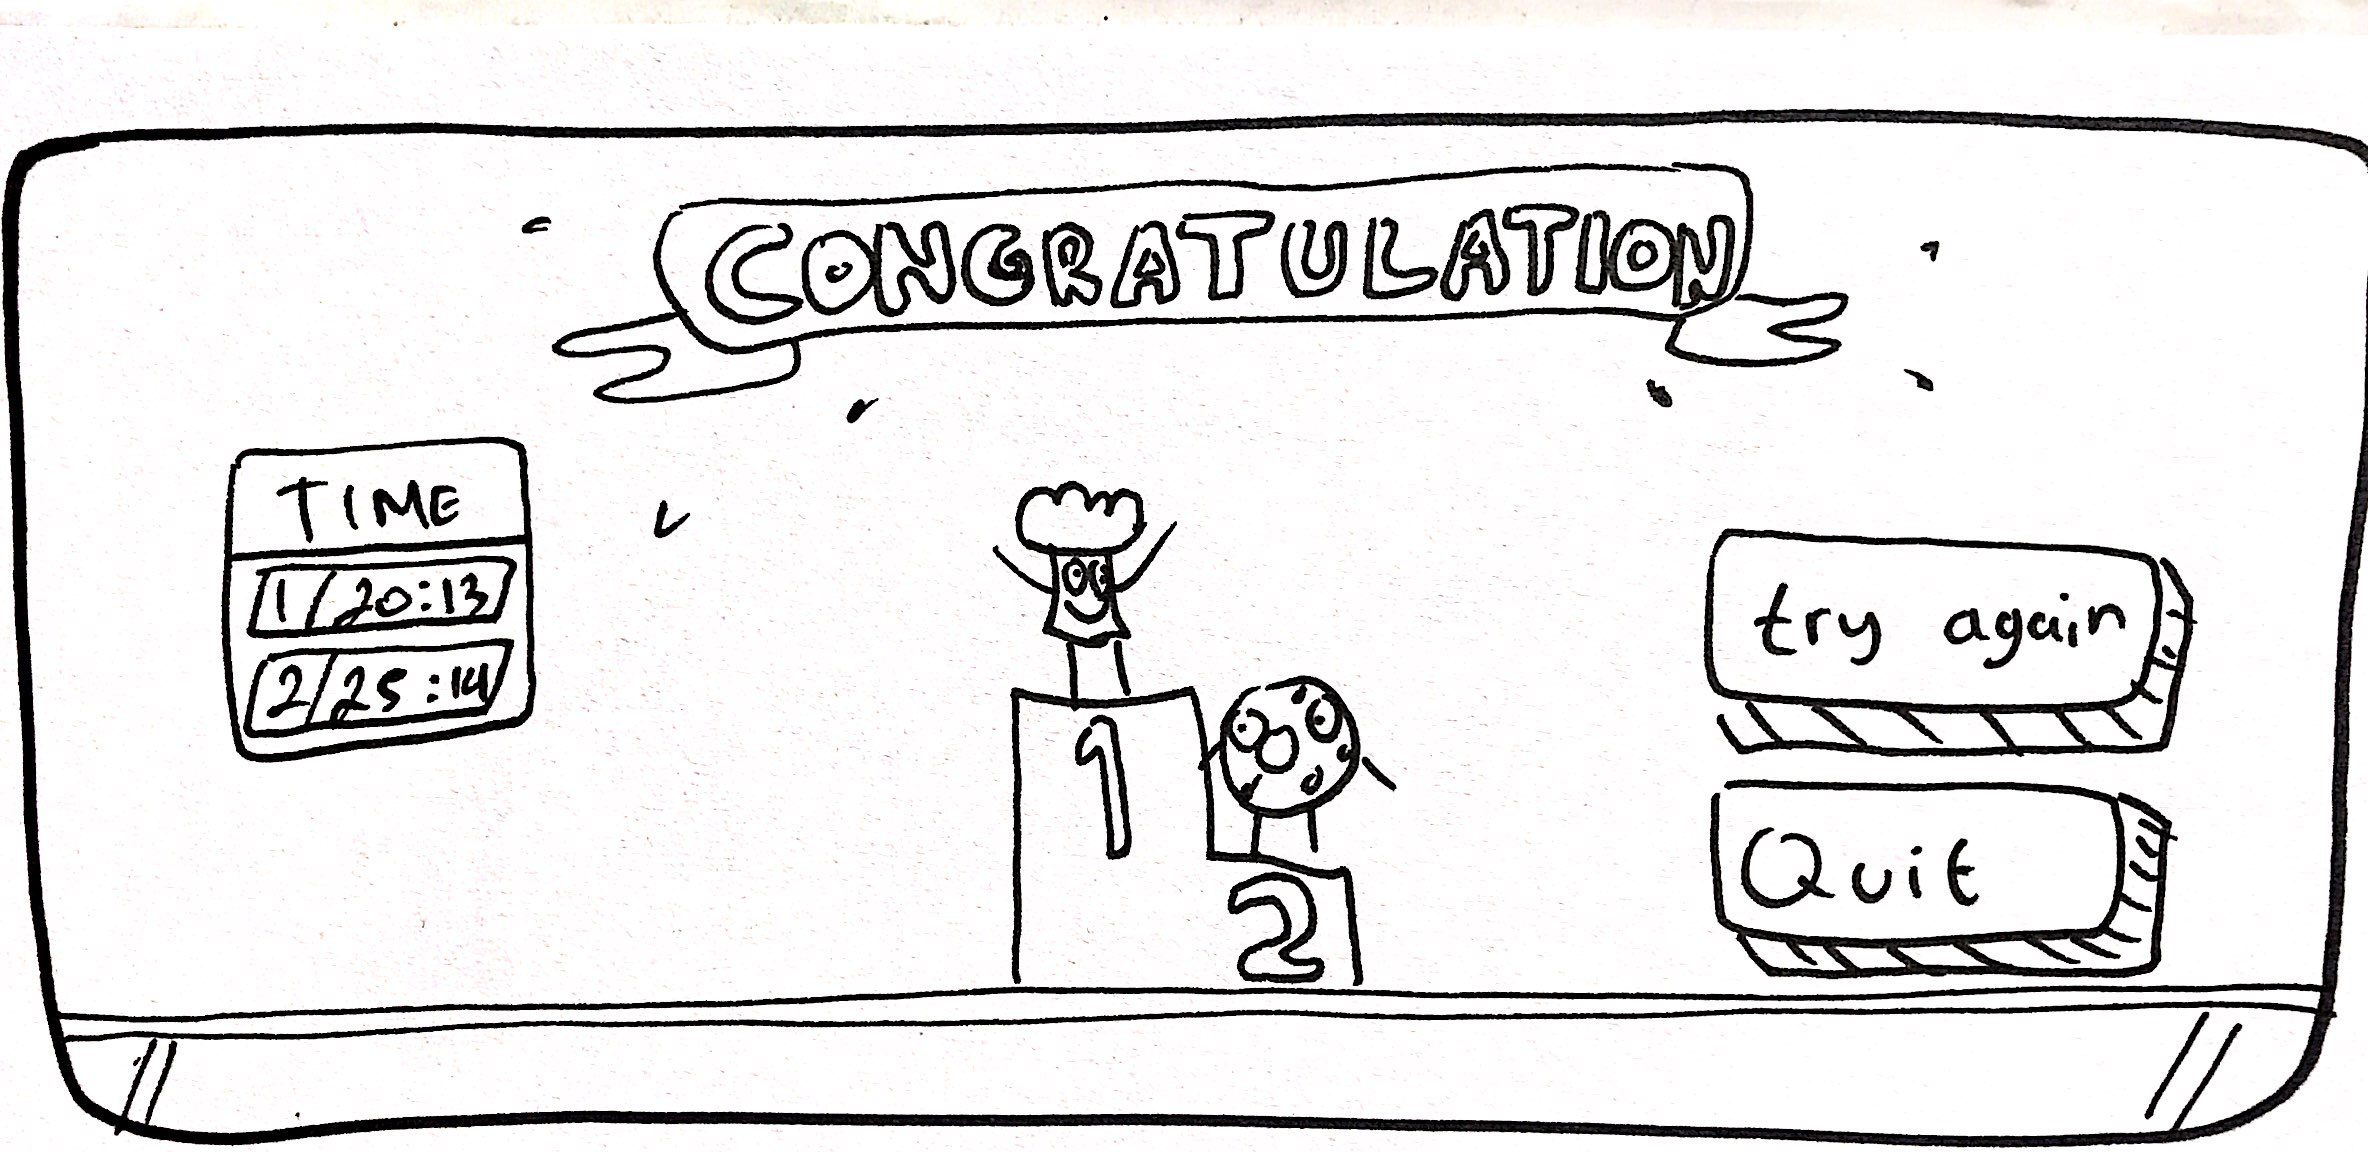
\includegraphics[scale=0.1]{Gambar/web9_end1}
			\caption{Permainan sudah selesai}
			\label{fig:9_web9_end1}
		\end{figure}
	
		\textbf{SMARTPHONE}
		
		\begin{figure}[H]
			\centering
			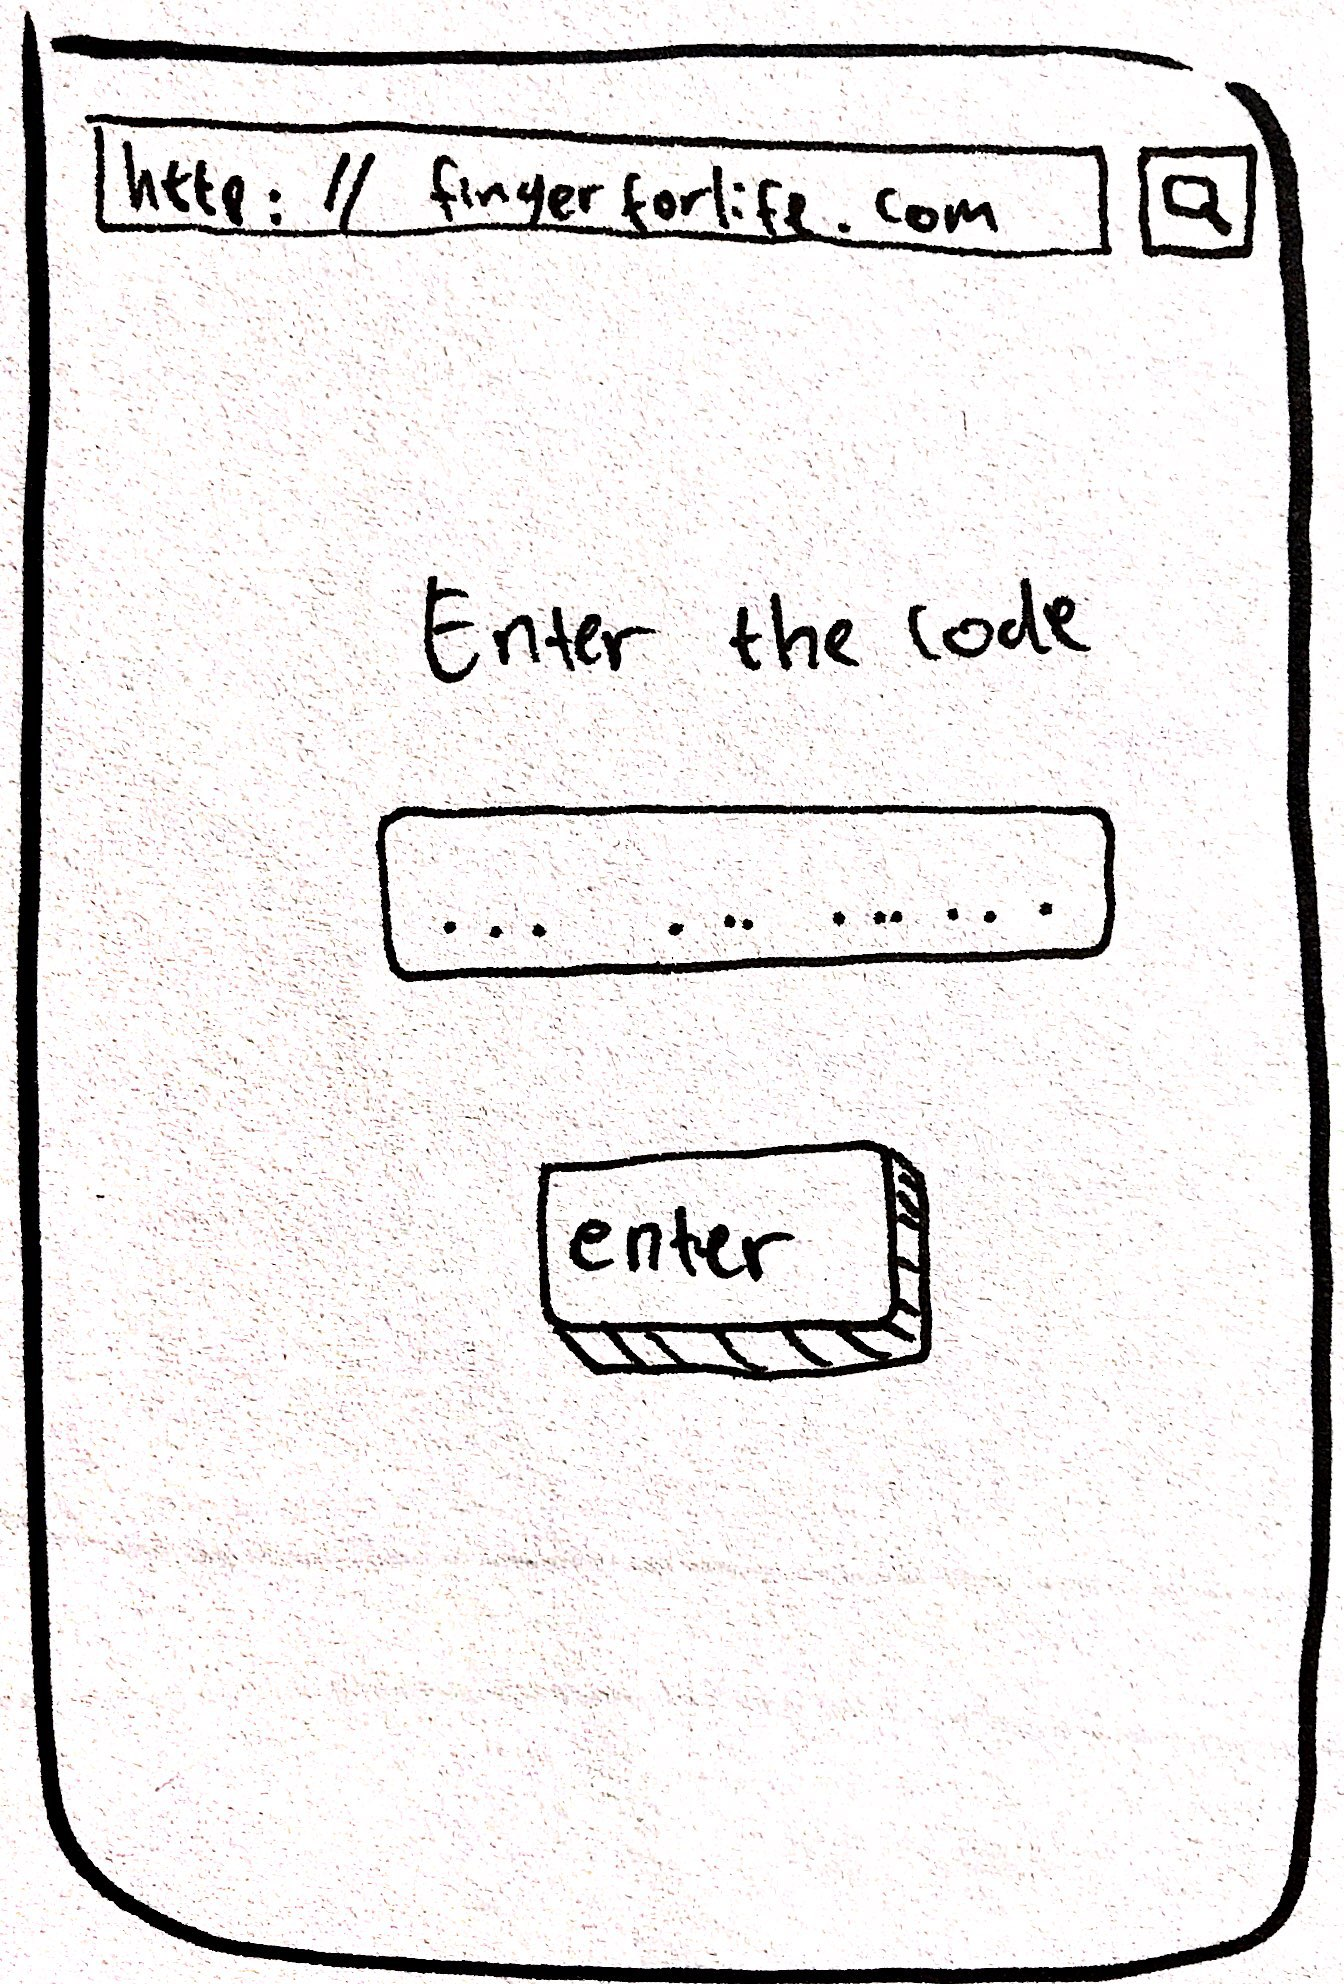
\includegraphics[scale=0.1]{Gambar/mob1_home1}
			\caption{Pemain mengakses halaman web pada \textit{mobile browser}.}
			\label{fig:10_mob1_home1}
		\end{figure}
	
		\begin{figure}[H]
			\centering
			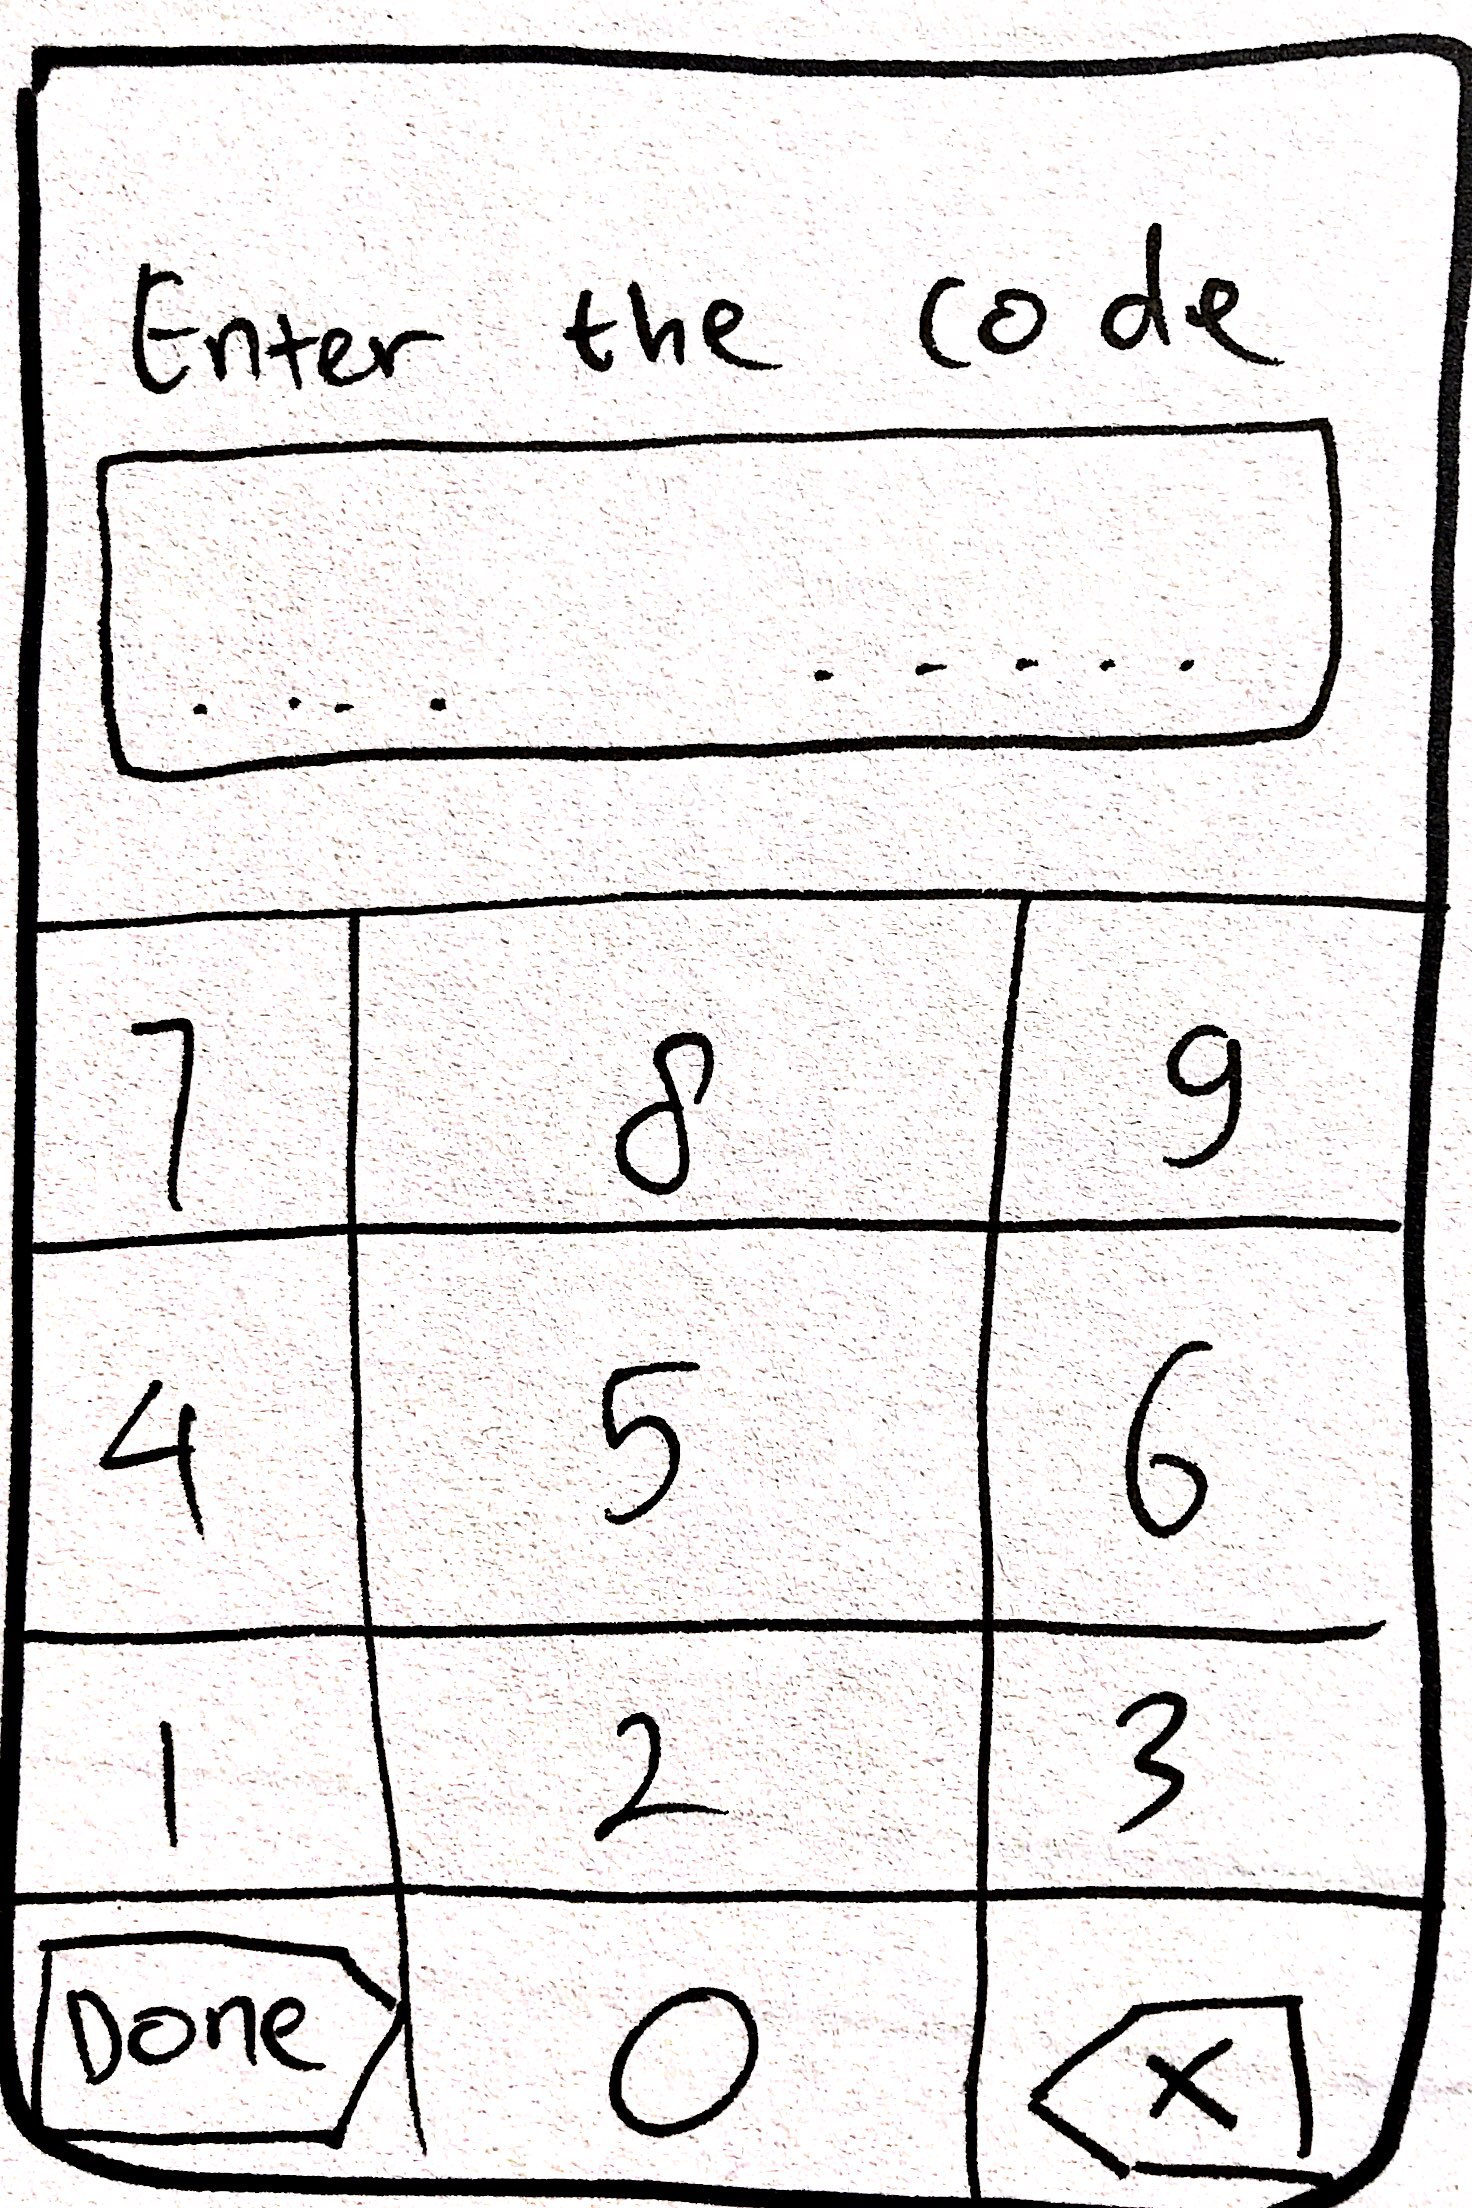
\includegraphics[scale=0.1]{Gambar/mob2_home2}
			\caption{Pemain memasukan kode yang didapatkan pada halaman web di \textit{PC}.}
			\label{fig:11_mob2_home2}
		\end{figure}
	
		\begin{figure}[H]
			\centering
			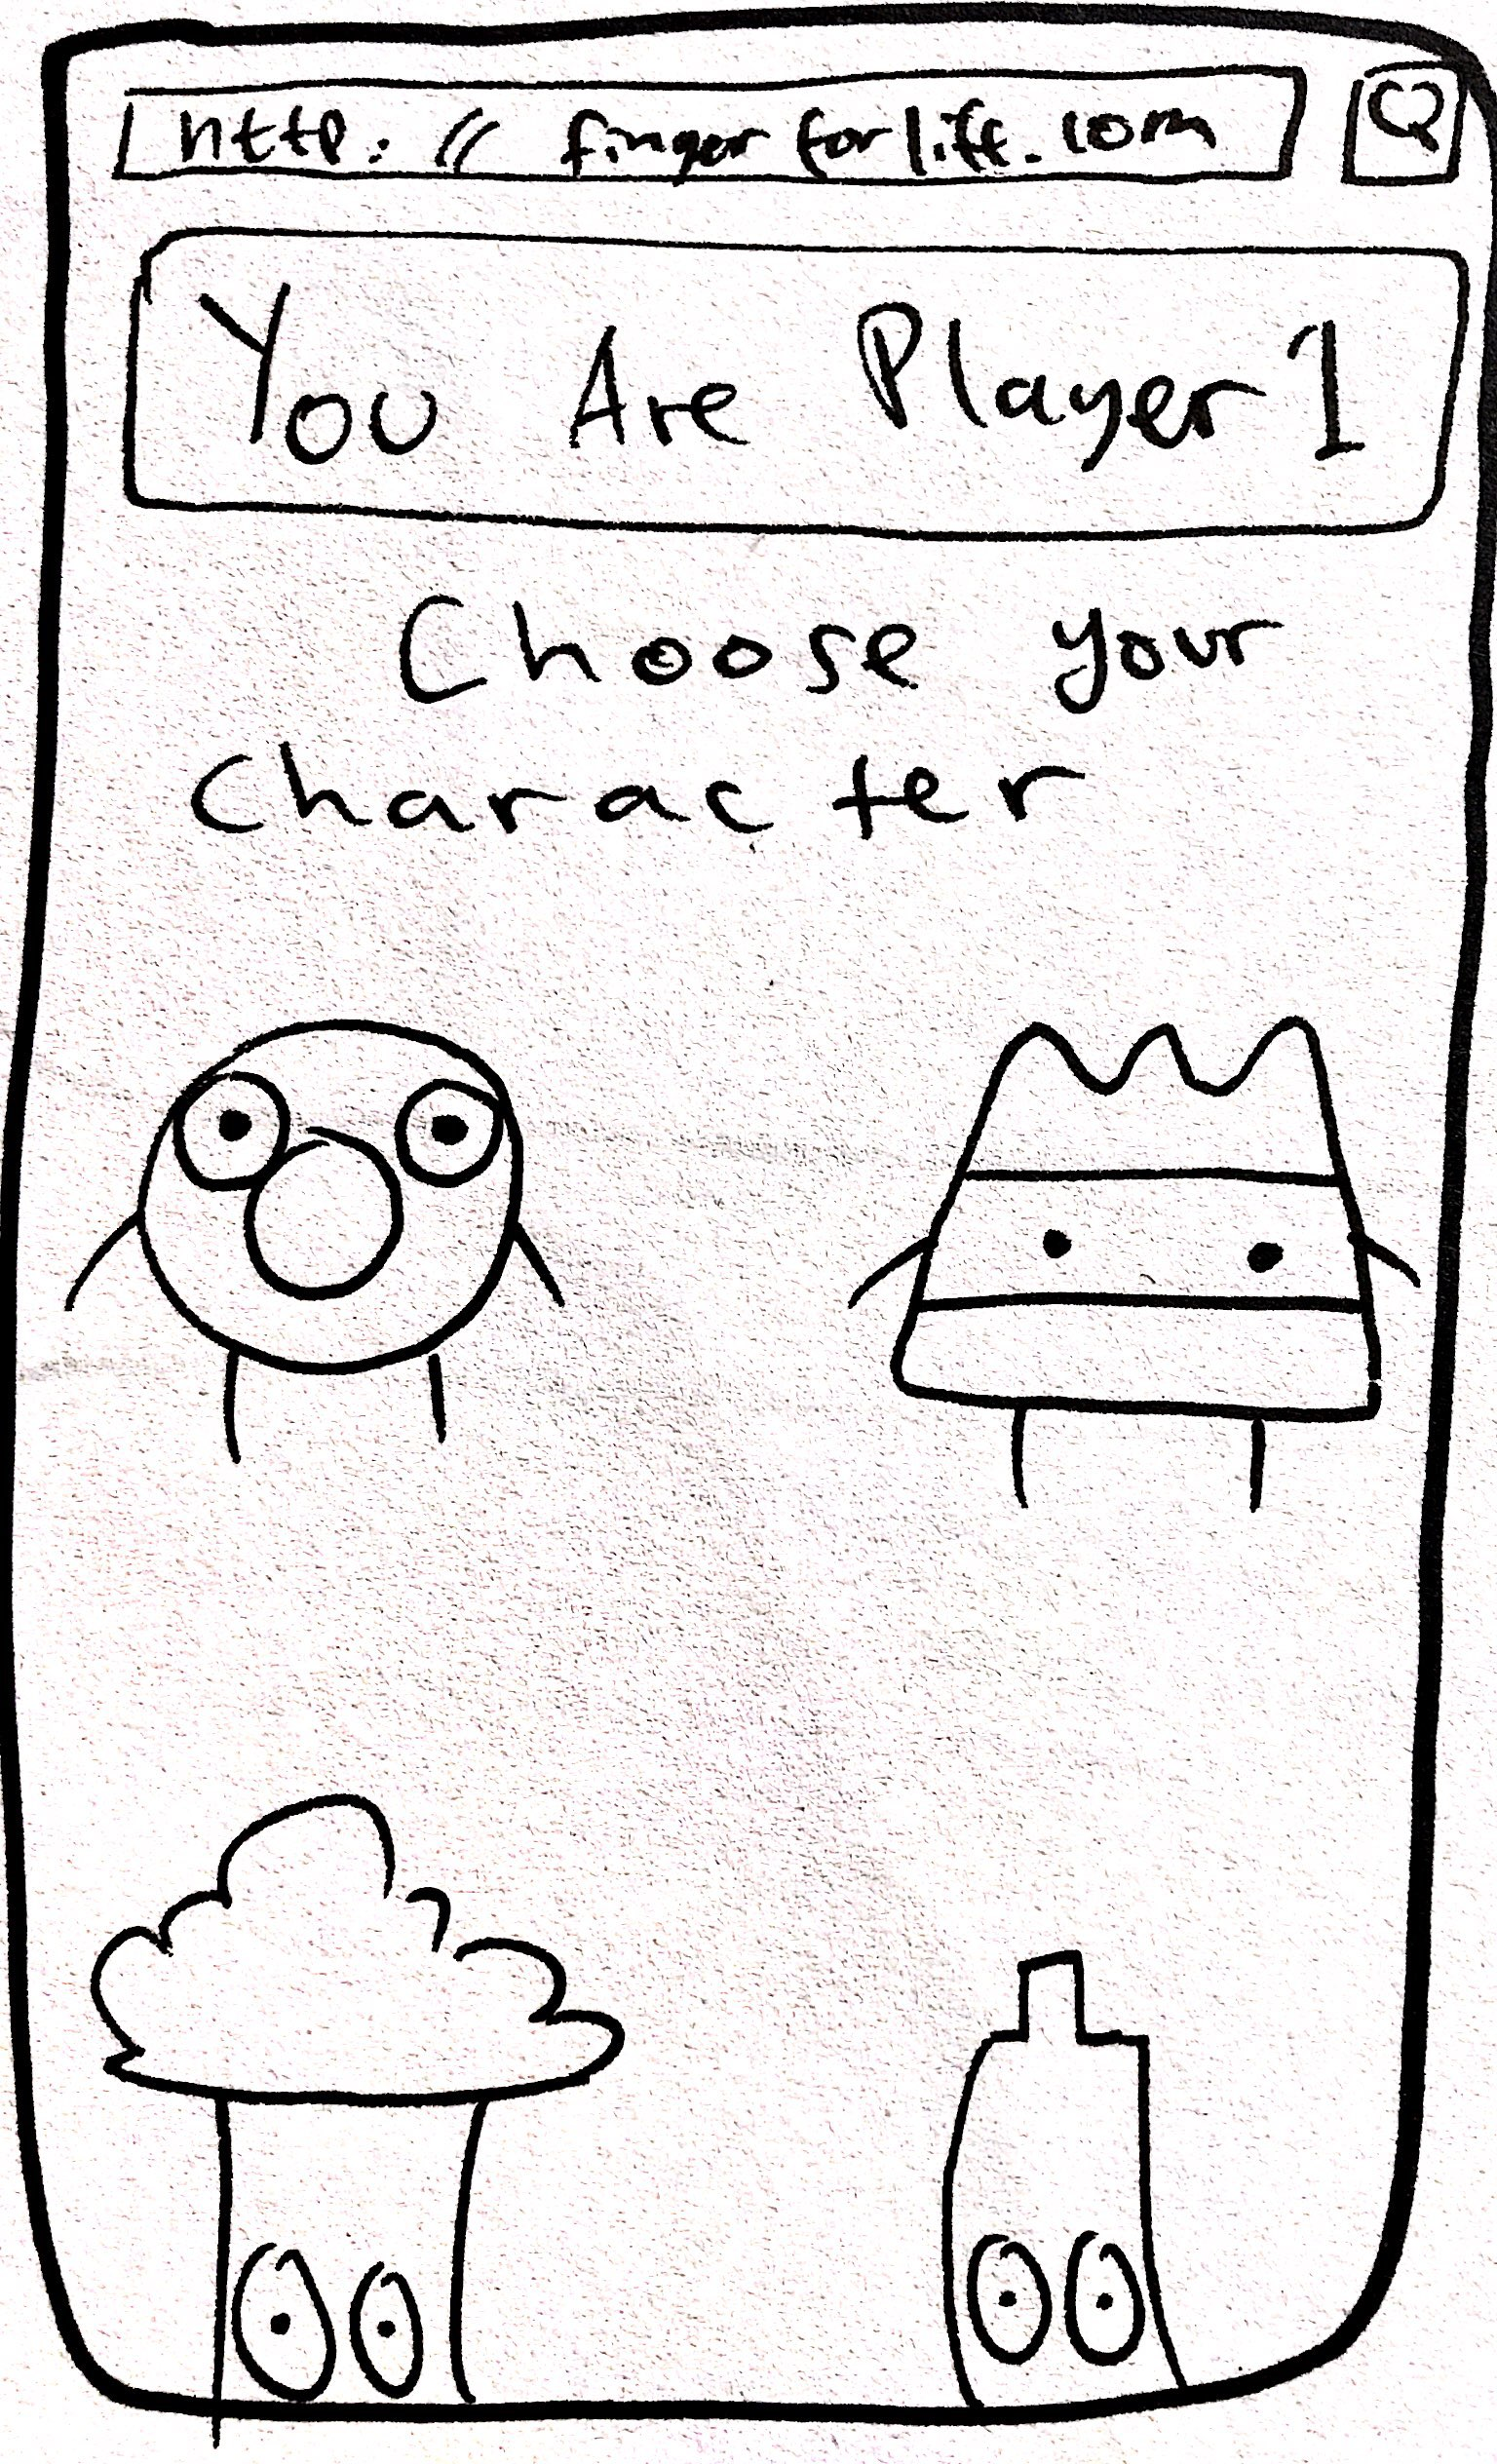
\includegraphics[scale=0.1]{Gambar/mob3_char1}
			\caption{Pemain memilih karakter yang akan dimainkan.}
			\label{fig:12_mob3_char1}
		\end{figure}
	
		\begin{figure}[H]
			\centering
			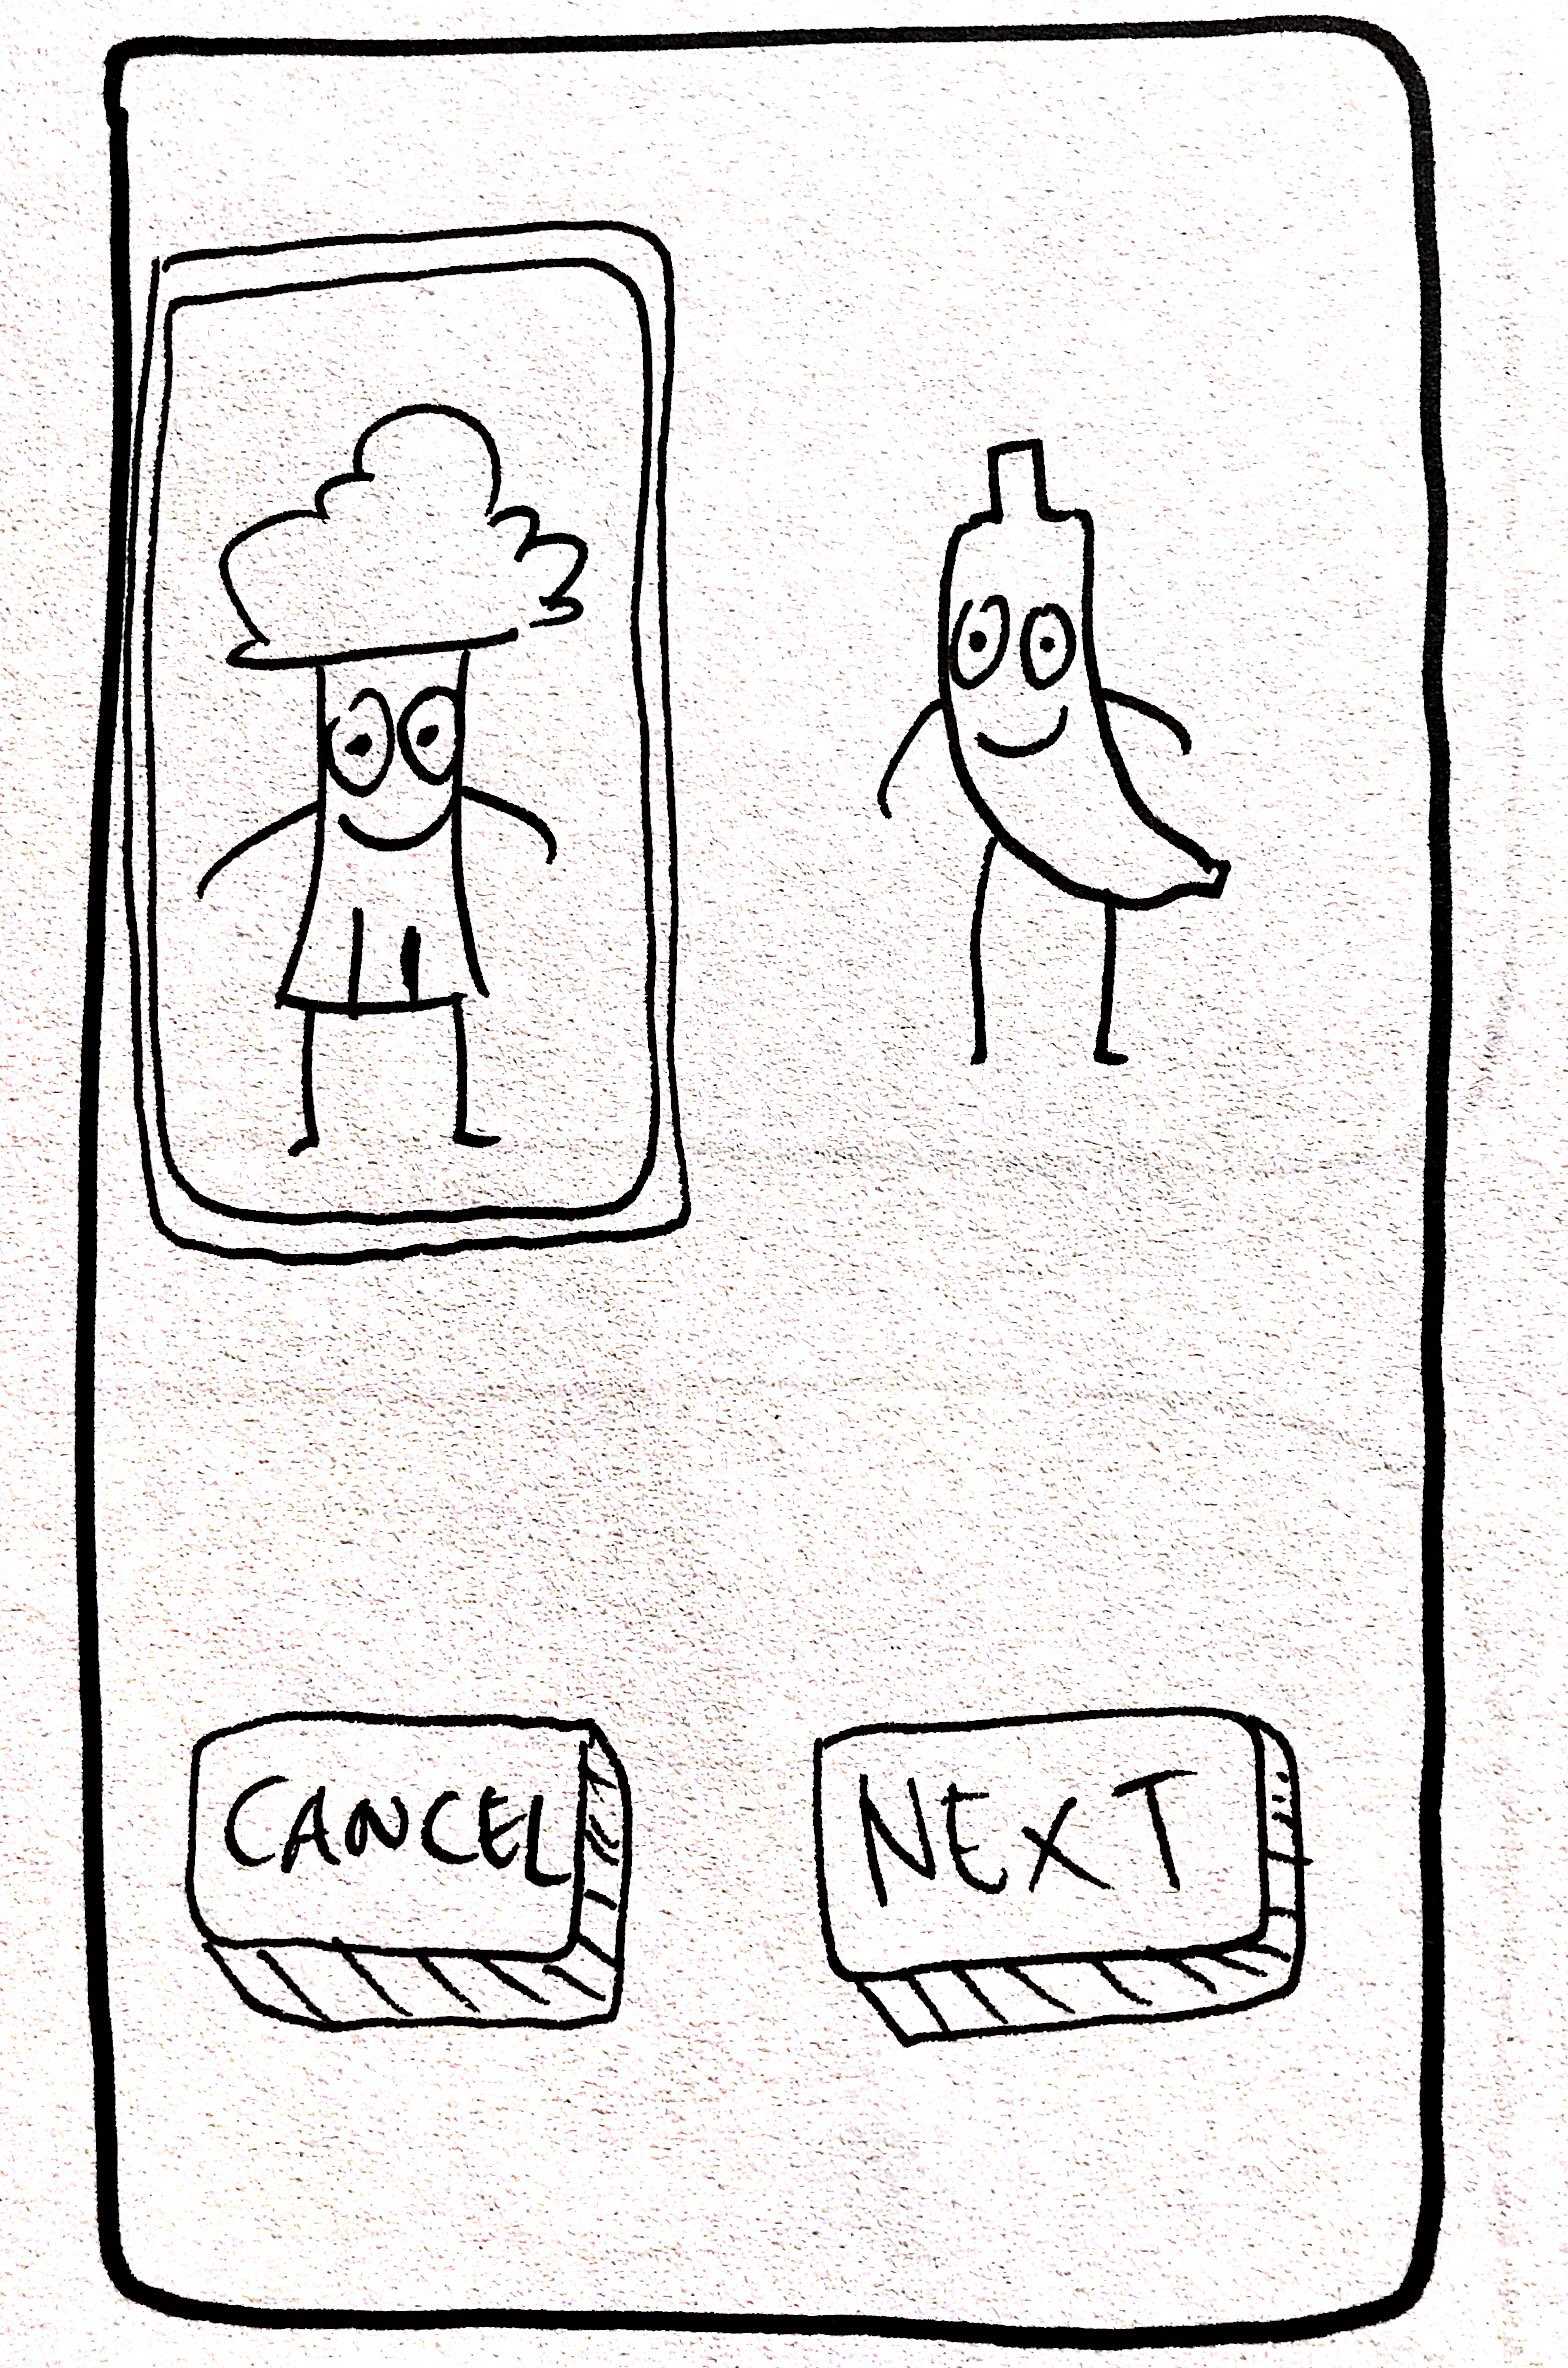
\includegraphics[scale=0.1]{Gambar/mob4_char2}
			\caption{Pemain menentukan karakter.}
			\label{fig:13_mob4_char2}
		\end{figure}
	
		\begin{figure}[H]
			\centering
			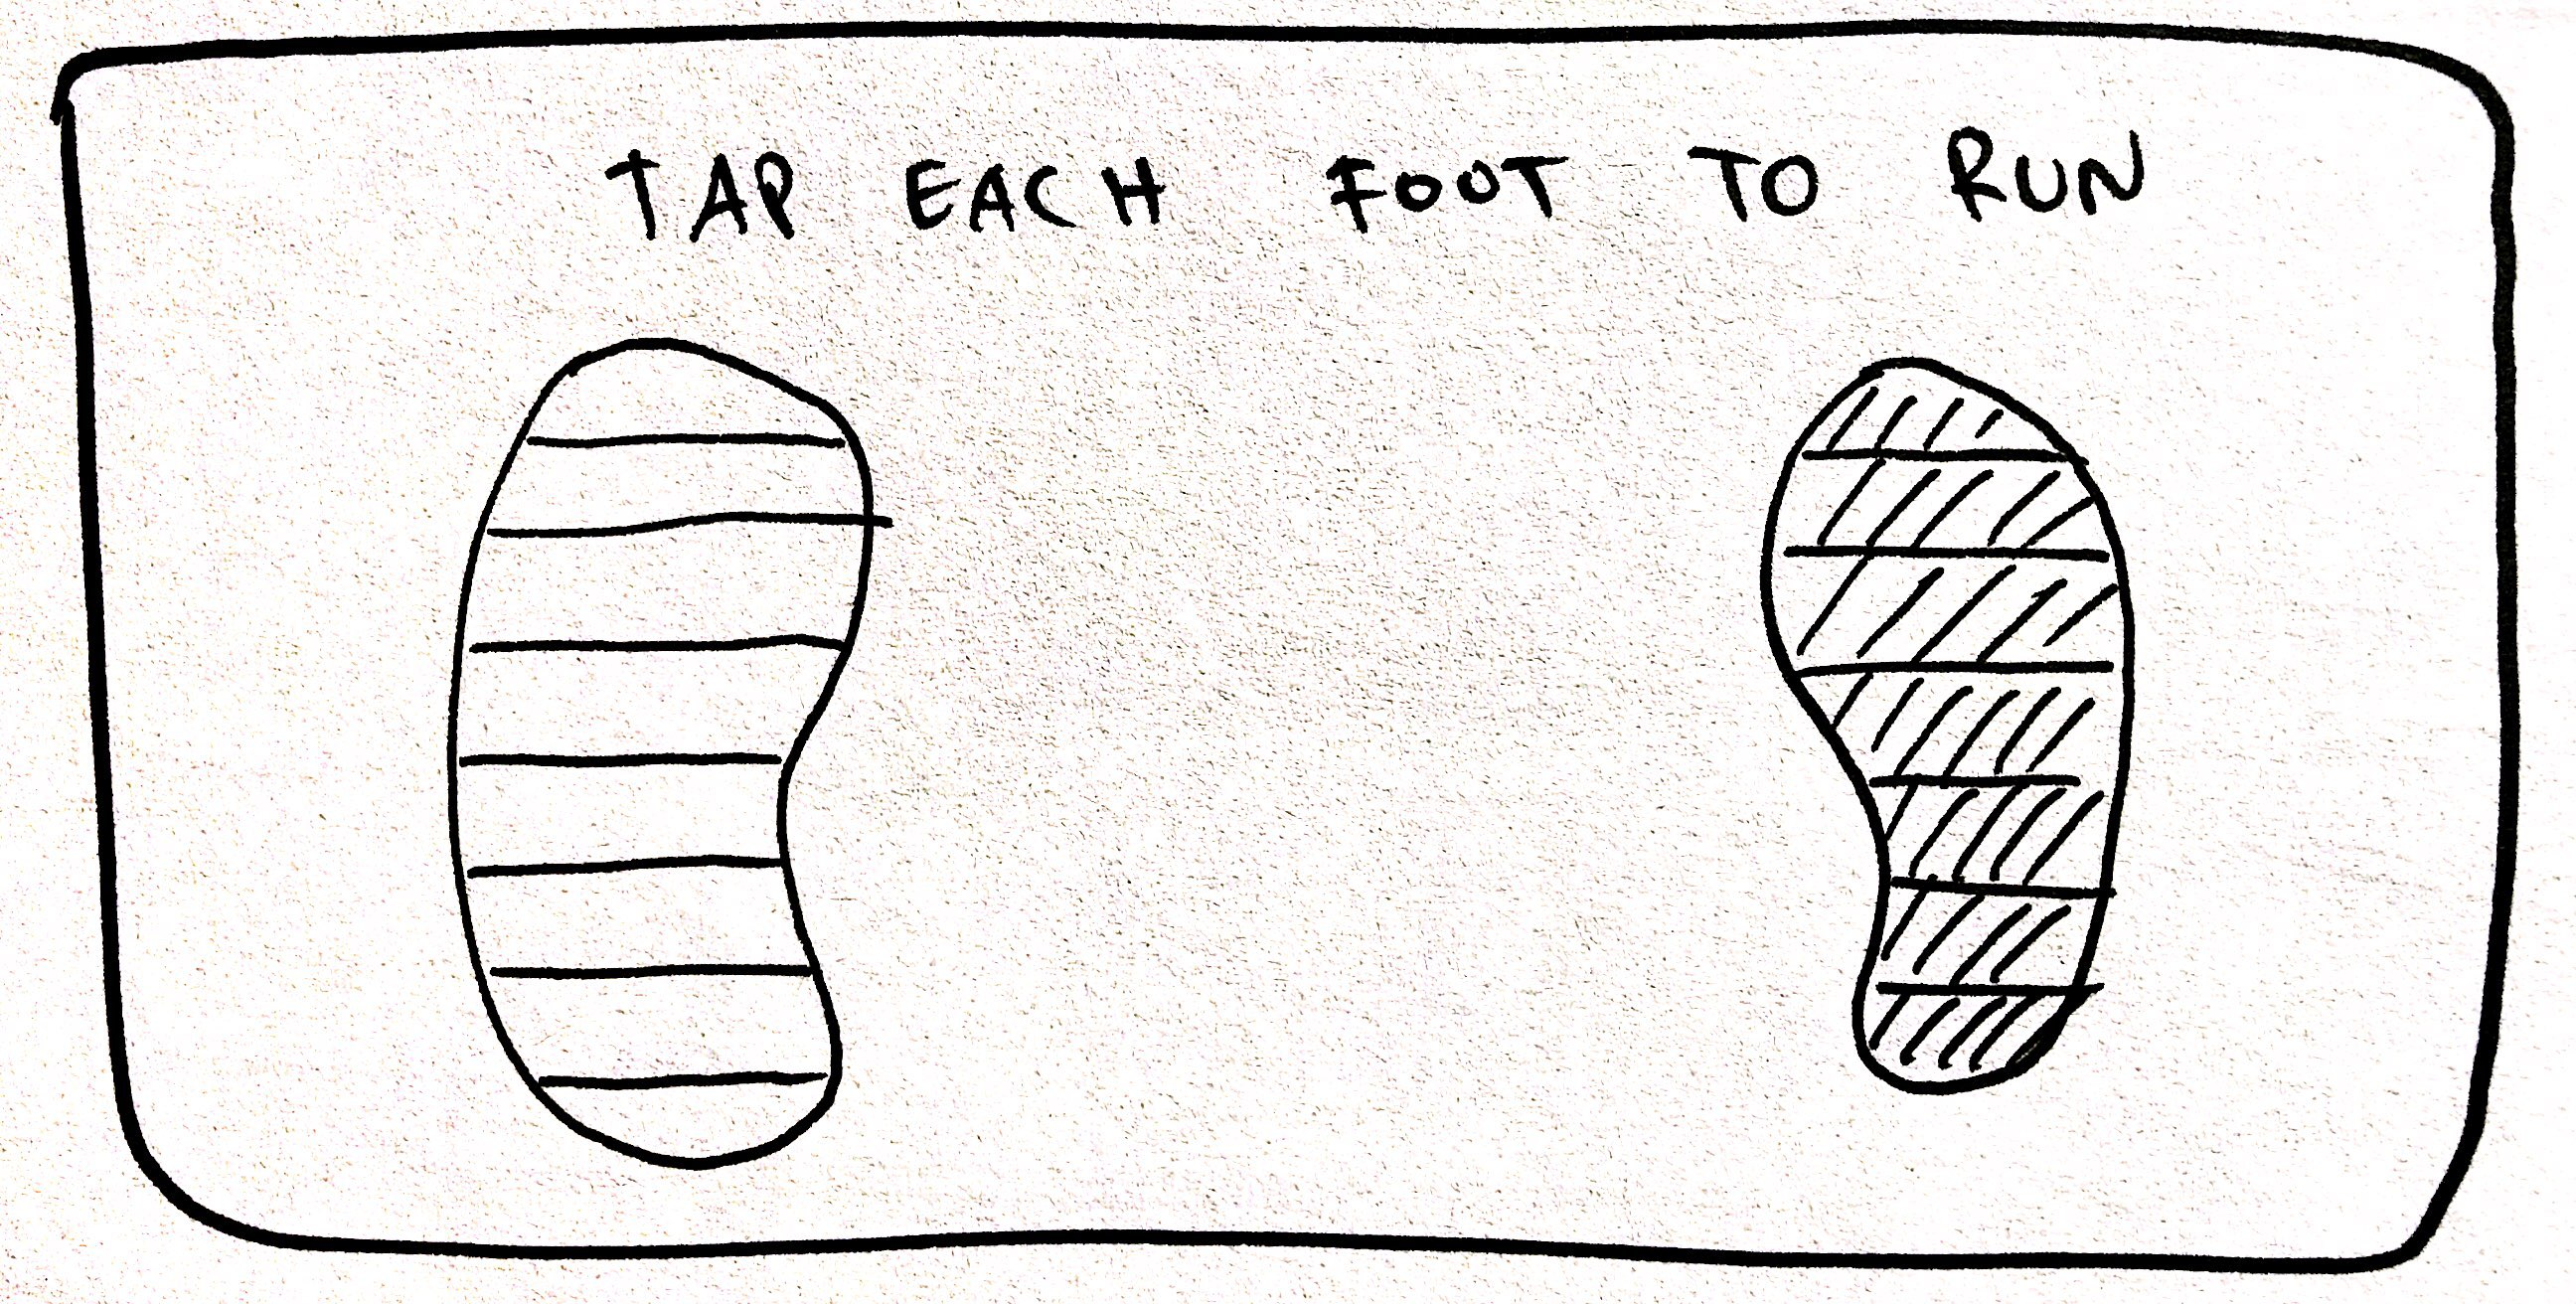
\includegraphics[scale=0.1]{Gambar/mob5_play}
			\caption{Pemain mulai memainkan permainan.}
			\label{fig:14_mob5_play}
		\end{figure}
	
		\begin{figure}[H]
			\centering
			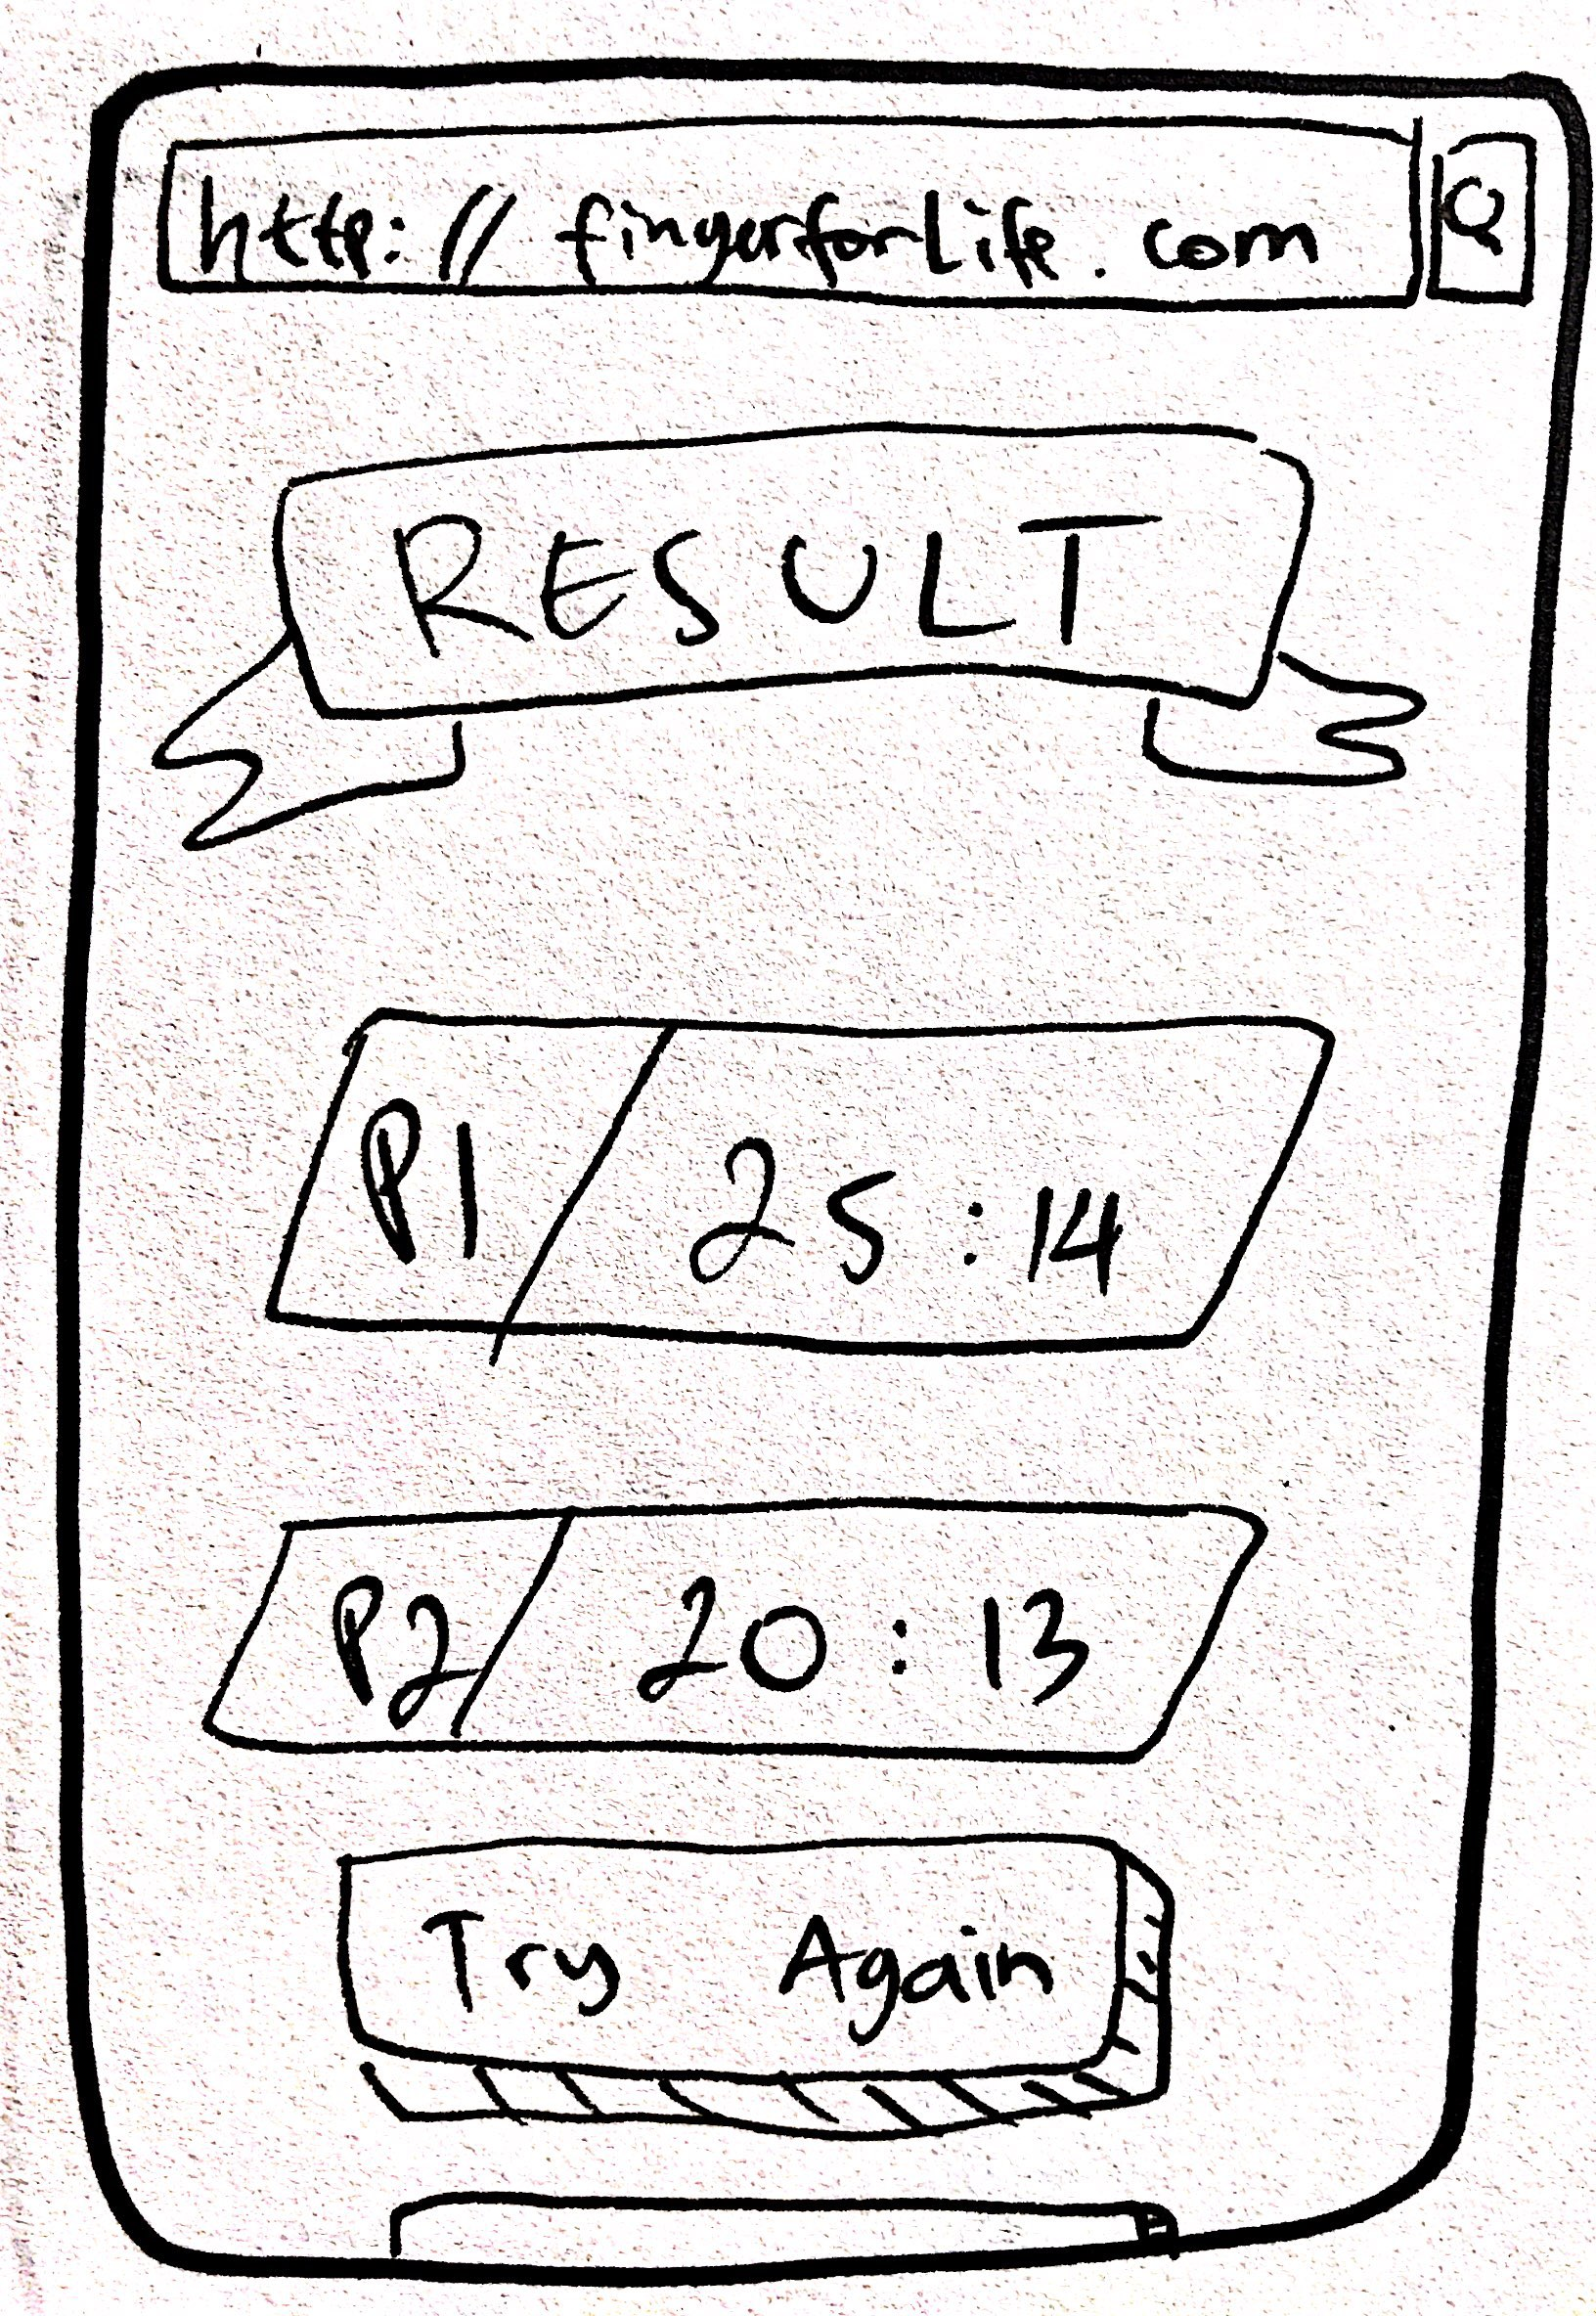
\includegraphics[scale=0.1]{Gambar/mob6_end}
			\caption{Permainan berakhir.}
			\label{fig:15_mob6_end}
		\end{figure}

		\item Menyusun cara bermain aplikasi permainan yang dibangun. \\
		{\bf status :} Ada sejak rencana kerja skripsi.\\
		{\bf hasil :} \\ 
		Pada skripsi ini, akan dibuat sebuah aplikasi permainan yang memanfaatkan protokol \textit{WebSockets}, dimana dalam penggunaan protokol tersebut akan dibantu dengan teknologi \textit{Socket.io}. Selain itu, aplikasi yang dibuat akan memanfaatkan \textit{personal computer (PC)} dan \textit{smartphone} untuk pengembangan aplikasinya. Kedua teknologi tersebut merupakan teknologi yang sudah dimiliki oleh banyak orang. Oleh karena itu, aplikasi permainan yang akan dibangun akan memanfaatkan \textit{PC} dan \textit{smartphone}.
		
		Nama permainan yang akan dibangun adalah \textit{Finger For Life}. Permainan tersebut merupakan adu balap lari yang dapat dimainkan oleh dua orang pemain, dimana para pemain akan memiliki karakter untuk dimainkan pada trek lari yang berbentuk huruf S di layar \textit{PC}. Agar dapat memainkan permainan tersebut, para pemain harus memiliki \textit{smartphone} dan \textit{PC} beserta koneksi internet yang stabil. Apabila hal-hal tersebut terpenuhi, pemain dapat membuka \textit{web browser} pada \textit{PC} untuk mengakses alamat web yang akan menuju ke permainan \textit{Finger For Life}. Para pemain akan diminta untuk melakukan dua hal agar dapat memainkan permainan tersebut bersama seorang rekan yang akan menjadi lawan mainnya, yaitu : 
		
		\begin{itemize}
			\item Membuka \textit{web browser} pada \textit{PC} untuk mengakses alamat web permainan \textit{Finger For Life}.
			\item Mengakses alamat web permainan dan memasukan kode tertentu pada \textit{web browser} di \textit{smartphone} untuk sesi permainan saat ini.
		\end{itemize}
		
		Kedua hal tersebut bertujuan untuk melakukan koneksi antara \textit{smartphone} dan \textit{PC}, dimana \textit{smartphone} akan berfungsi sebagai \textit{controller} dalam permainan. Apabila kedua hal diatas telah dilakukan, maka kedua pemain akan dapat mulai memainkan permainannya.  Permainan akan diawali dengan pemilihan karakter oleh kedua pemain, dimana karakter tersebut akan berfungsi sebagai representasi masing-masing pemain dalam permainan \textit{Finger For Life}. Setelah pemilihan karakter selesai, maka para pemain akan dibawa ke halaman selanjutnya yang berupa halaman \textit{game on}. Pada halaman ini, para pemain diminta untuk memegang \textit{smartphone} masing-masing untuk mencoba memainkan permainannya dengan cara menekan tombol-tombol yang muncul pada \textit{smartphone}. Hal tersebut bertujuan agar para pemain terbiasa terlebih dahulu dengan cara bermainnya. Setelah hal itu dilakukan, maka para pemain dapat memulai memainkan permainannya.
		
		Para pemain akan mengkoneksikan \textit{smartphone} miliknya pada suatu \textit{PC}, dimana \textit{smartphone} tersebut akan berfungsi sebagai \textit{controller} untuk memainkan permainannya. Oleh karena itu, protokol \textit{WebSockets} akan digunakan sebagai koneksi antara \textit{smartphone} dan \textit{PC} dalam aplikasi permainan yang akan dibangun. Aplikasi permainan akan menggunakan teknologi berbasis web, sehingga untuk memainkannya, \textit{client} bisa mengakses melalui \textit{web browser} tanpa harus berada di satu jaringan lokal yang sama.

		\item Mengimplementasi program aplikasi permainan berbasis web. \\
		{\bf status :} Ada sejak rencana kerja skripsi.\\
		{\bf hasil :} -
		

		\item Menganalisis \textit{latency} yang dihasilkan pada aplikasi.\\
		{\bf status :} Ada sejak rencana kerja skripsi.\\
		{\bf hasil :} -

		\item Melakukan eksperimen dan pengujian yang melibatkan responden.\\
		{\bf status :} Ada sejak rencana kerja skripsi.\\
		{\bf hasil :} -

		\item Menulis dokumen skripsi\\
		{\bf status :} Ada sejak rencana kerja skripsi.\\
		{\bf hasil :} Dokumen sudah ditulis dari bab1 hingga bab2.
		

	\end{enumerate}

%\bibliographystyle{ieeetr}
\bibliographystyle{compj} %gunakan compj 
\bibliography{referensi}

\section{Pencapaian Rencana Kerja}
Persentase penyelesaian skripsi sampai dengan dokumen ini dibuat dapat dilihat pada tabel berikut :

\begin{center}
  \begin{tabular}{ | c | c | c | c | l | c |}
    \hline
    1*  & 2*(\%) & 3*(\%) & 4*(\%) &5* &6*(\%)\\ \hline \hline
    1   & 10  & 10  &  &  & 10 \\ \hline
    2   & 5 & 5  &   &  & 1 \\ \hline
    3   & 10  & 5  & 5 &  & 5 \\ \hline
    4   & 15  & 5  &  10 & & 5 \\ \hline
    5   & 20  & 5  & 15 & & 1 \\ \hline
    6   & 10 &   & 10  &  & \\\hline
    7   & 10  &   & 10 &  &  \\ \hline
    8   & 20  & 10 & 10  & 6 {\footnotesize menulis dokumen skripsi dari bab1 hingga bab3 di S1}  &\\ \hline
    Total  & 100  & 40  & 60 &  & 28\\ \hline
                          \end{tabular}
\end{center}

Keterangan (*)\\
1 : Bagian pengerjaan Skripsi (nomor disesuaikan dengan detail pengerjaan di bagian 5)\\
2 : Persentase total \\
3 : Persentase yang akan diselesaikan di Skripsi 1 \\
4 : Persentase yang akan diselesaikan di Skripsi 2 \\
5 : Penjelasan singkat apa yang dilakukan di S1 (Skripsi 1) atau S2 (skripsi 2)\\
6 : Persentase yang sidah diselesaikan sampai saat ini 

\vspace{1cm}
\centering Bandung, \tanggal\\
\vspace{2cm} \nama \\ 
\vspace{1cm}

Menyetujui, \\
\ifdefstring{\jumpemb}{2}{
\vspace{1.5cm}
\begin{centering} Menyetujui,\\ \end{centering} \vspace{0.75cm}
\begin{minipage}[b]{0.45\linewidth}
% \centering Bandung, \makebox[0.5cm]{\hrulefill}/\makebox[0.5cm]{\hrulefill}/2013 \\
\vspace{2cm} Nama: \pembA \\ Pembimbing Utama
\end{minipage} \hspace{0.5cm}
\begin{minipage}[b]{0.45\linewidth}
% \centering Bandung, \makebox[0.5cm]{\hrulefill}/\makebox[0.5cm]{\hrulefill}/2013\\
\vspace{2cm} Nama: \pemB \\ Pembimbing Pendamping
\end{minipage}
\vspace{0.5cm}
}{
% \centering Bandung, \makebox[0.5cm]{\hrulefill}/\makebox[0.5cm]{\hrulefill}/2013\\
\vspace{2cm} Nama: \pembA \\ Pembimbing Tunggal
}

\end{document}

